% DD2350 ADK -- Övning 10: NP-fullständiga problem
% Beamer-presentation, pdflatex, 16:9
% Bildfiler som ska ligga bredvid den här filen:
%   KTH_logo_RGB_bla.png, hastad-kort.jpg, hastad-lada.jpg
% (saknas någon av dem kompilerar filen ändå, med en platshållare).
\documentclass[aspectratio=169,10pt]{beamer}

\usepackage[utf8]{inputenc}
\usepackage[T1]{fontenc}
\usepackage[swedish]{babel}
\usepackage{helvet}
\renewcommand{\familydefault}{\sfdefault}
% Latin Modern för skrivmaskinsstil och rak stil i matematik: samma utseende som
% Computer Modern, men alltid vektorfonter (inga bitmappar i pdf-filen).
\renewcommand{\rmdefault}{lmr}
\renewcommand{\ttdefault}{lmtt}
\usepackage{amsmath,amssymb}
\usepackage{booktabs}
\usepackage{array}
\newcolumntype{L}[1]{>{\raggedright\arraybackslash}p{#1}}
\usepackage{listings}
\usepackage{tikz}
\usetikzlibrary{arrows.meta,positioning,matrix,calc,fit,shapes.geometric,decorations.pathreplacing,backgrounds}

% Babel gör " aktivt på svenska; vi använder inte de kortformerna.
\AtBeginDocument{\shorthandoff{"}}

% ---------- Färger (KTH-blått + några accenter) ----------
\definecolor{kthblue}{HTML}{1954A6}
\definecolor{kthsky}{HTML}{24A0D8}
\definecolor{okgreen}{HTML}{62922E}
\definecolor{warnorange}{HTML}{E07B1C}
\definecolor{badred}{HTML}{B4232B}
\definecolor{softgray}{HTML}{8A8A8A}
% Kortfärger till Håstads pussel (bakgrund och markering för igenfyllt hål)
\colorlet{kortbg}{warnorange!25}\colorlet{kortm}{black!17!kortbg}
\colorlet{kortvandbg}{warnorange!58}\colorlet{kortvandm}{black!17!kortvandbg}
\colorlet{kortextrabg}{kthsky!28}\colorlet{kortextram}{black!17!kortextrabg}
\colorlet{kortextravandbg}{kthsky!60}\colorlet{kortextravandm}{black!17!kortextravandbg}
\colorlet{korthogbg}{black!14}\colorlet{korthogm}{black!17!korthogbg}

% ---------- Beamer-tema ----------
\usetheme{default}
\setbeamertemplate{navigation symbols}{}
\setbeamercolor{structure}{fg=kthblue}
\setbeamercolor{title}{fg=kthblue}
\setbeamercolor{frametitle}{bg=kthblue,fg=white}
\setbeamercolor{footline}{fg=softgray}
\setbeamercolor{alerted text}{fg=badred}
\setbeamercolor{block title}{bg=kthblue,fg=white}
\setbeamercolor{block body}{bg=kthblue!8}
\setbeamercolor{block title example}{bg=okgreen,fg=white}
\setbeamercolor{block body example}{bg=okgreen!10}
\setbeamercolor{block title alerted}{bg=warnorange,fg=white}
\setbeamercolor{block body alerted}{bg=warnorange!10}
\setbeamertemplate{itemize items}[circle]
\setbeamertemplate{enumerate items}[default]
\setbeamertemplate{blocks}[rounded][shadow=false]
\setbeamerfont{frametitle}{size=\large,series=\bfseries}
\setbeamerfont{title}{size=\LARGE,series=\bfseries}
\setbeamerfont{block title}{size=\normalsize,series=\bfseries}

% Bildfiler: använd dem om de finns, annars en platshållare.
\newcommand{\kthlogo}[1]{\IfFileExists{KTH_logo_RGB_bla.png}{
\includegraphics[height=#1]{KTH_logo_RGB_bla.png}}{\textcolor{kthblue}{\bfseries KTH}}}
\newcommand{\foto}[2]{\IfFileExists{#2}{\includegraphics[#1]{#2}}{\fbox{\scriptsize\strut bildfilen #2 saknas}}}

% Rubrikbalk i KTH-blått över hela bredden
\makeatletter
\setbeamertemplate{frametitle}{%
  \nointerlineskip
  \begin{beamercolorbox}[wd=\paperwidth,sep=0.2cm,leftskip=0.5cm,rightskip=0.5cm]{frametitle}
    \usebeamerfont{frametitle}\insertframetitle%
    \ifx\insertframesubtitle\@empty\else\hfill{\small\mdseries\insertframesubtitle}\fi
  \end{beamercolorbox}}
\makeatother

% Sidfot med KTH-logga
\setbeamertemplate{footline}{%
  \leavevmode%
  \begin{beamercolorbox}[wd=\paperwidth,ht=0.62cm,dp=0.13cm,leftskip=0.5cm,rightskip=0.5cm]{footline}
    \kthlogo{0.5cm}%
    \hspace{0.3cm}\raisebox{0.18cm}{\scriptsize DD2350 ADK -- Övning 10: NP-fullständiga problem}%
    \hfill\raisebox{0.18cm}{\scriptsize Marcus Dicander}%
    \hfill\raisebox{0.18cm}{\scriptsize\insertframenumber\,/\,\inserttotalframenumber}%
  \end{beamercolorbox}}

% Titelsida
\setbeamertemplate{title page}{%
  \vfill
  \begin{center}
    \kthlogo{2.2cm}\\[1.2em]
    {\usebeamerfont{title}\usebeamercolor[fg]{title}\inserttitle\par}
    \vspace{0.4em}
    {\large\insertsubtitle\par}
    \vspace{1.2em}
    {\insertauthor\par}
    \vspace{0.3em}
    {\small\insertdate\par}
  \end{center}
  \vfill}

% Sektionssida
\setbeamertemplate{section page}{%
  \vfill
  \begin{beamercolorbox}[wd=\paperwidth,sep=0.6cm,center]{frametitle}
    {\usebeamerfont{title}\insertsection\par}
  \end{beamercolorbox}
  \vfill}
\AtBeginSection[]{\begin{frame}[plain]\sectionpage\end{frame}}

% ---------- Overlay-stilar i TikZ ----------
\tikzset{
  invisible/.style={opacity=0,text opacity=0},
  visible on/.style={alt=#1{}{invisible}},
  alt/.code args={<#1>#2#3}{\alt<#1>{\pgfkeysalso{#2}}{\pgfkeysalso{#3}}},
  textinvisible/.style={text opacity=0},
  text on/.style={alt=#1{}{textinvisible}},
  % gemensamma ritstilar
  cell/.style={draw=black!70,minimum size=7mm,inner sep=0pt,font=\small},
  smallcell/.style={draw=black!70,minimum size=5.5mm,inner sep=0pt,font=\scriptsize},
  hdr/.style={minimum size=5.5mm,inner sep=0pt,font=\scriptsize\bfseries,text=kthblue},
  hl/.style={fill=kthblue!25},
  hlok/.style={fill=okgreen!30},
  hlwarn/.style={fill=warnorange!35},
  hlbad/.style={fill=badred!25},
  dep/.style={-{Stealth[length=2mm]},thick,kthblue},
  path/.style={-{Stealth[length=2.5mm]},line width=1.6pt,okgreen},
  bad/.style={-{Stealth[length=2.5mm]},line width=1.4pt,badred,dashed},
  lab/.style={font=\scriptsize,text=black!70},
  % grafer
  vx/.style={circle,draw=black!70,fill=white,minimum size=5.5mm,inner sep=0pt,font=\scriptsize},
  ed/.style={black!40,line width=0.7pt},
  sel/.style={kthblue,line width=1.9pt},
  pA/.style={okgreen,line width=1.9pt},
  pB/.style={warnorange,line width=1.9pt},
  pC/.style={kthsky,line width=1.9pt},
  % lådor och pilar i flödesbilder
  bx/.style={draw=black!70,rounded corners=2pt,minimum height=7.5mm,inner xsep=5pt,font=\small,fill=white,align=flush center},
  orakel/.style={draw=black,fill=black!85,text=white,rounded corners=2pt,minimum height=8mm,minimum width=12mm,font=\small\bfseries,align=center},
  flow/.style={-{Stealth[length=2mm]},thick,black!70},
  % tidsenheter (uppgift 4)
  t1/.style={fill=kthblue!30},
  t2/.style={fill=okgreen!40},
  t3/.style={fill=warnorange!45},
  t4/.style={fill=badred!28},
  % Håstads kort (uppgift 3). Varje stil X har en bakgrundsfärg Xbg och en färg Xm
  % för markeringen av ett igenfyllt hål.
  kort/.style={draw=warnorange!55!black,fill=kortbg,line width=0.5pt},
  kortvand/.style={draw=warnorange!55!black,fill=kortvandbg,line width=0.5pt},
  kortextra/.style={draw=kthblue!85,fill=kortextrabg,line width=0.5pt},
  kortextravand/.style={draw=kthblue!85,fill=kortextravandbg,line width=0.5pt},
  korthog/.style={draw=black!70,fill=korthogbg,line width=0.5pt},
  korthal/.style={draw=black!80,fill=white,line width=0.4pt},
  % lappar (uppgift 5)
  lapp/.style={draw=black!70,line width=0.5pt},
}

% Rutkoordinat: rad #1, kolumn #2, cellstorlek 8 mm, origo uppe till vänster
\newcommand{\cc}[2]{(#2*0.8-0.4,-#1*0.8+0.4)}

% Håstads kort: \hkort[tikz-val]{x}{y}{vänsterkolumn}{högerkolumn}{etikett}{stil}
% Kolumnerna är kommalistor uppifrån och ned, 1 = igenfyllt, 0 = hål.
% Rad j har sitt centrum på höjden  y + \kH - 0.62 - (j-0.5)*0.36.
\newcommand{\hkort}[7][]{%
  \begin{scope}[shift={(#2,#3)},#1]
    \foreach \b [count=\j] in {#4} {\xdef\kortm{\j}}%
    \pgfmathsetmacro{\kH}{0.62+\kortm*0.36+0.34}%
    \path[#7] (0,0) -- (0.52,0) -- (0.52,0.13) -- (0.78,0.13) -- (0.78,0) -- (1.3,0)
      -- (1.3,\kH-0.50) -- (1.17,\kH-0.50) -- (1.17,\kH-0.32) -- (1.3,\kH-0.32) -- (1.3,\kH)
      -- (0,\kH) -- (0,\kH-0.32) -- (0.13,\kH-0.32) -- (0.13,\kH-0.50) -- (0,\kH-0.50) -- cycle;
    \node[font=\scriptsize,inner sep=0pt] at (0.65,\kH-0.25) {#6};
    \foreach \b [count=\j] in {#4} {
      \ifnum\b=1 \path[fill=#7m] (0.38,\kH-0.44-\j*0.36) circle (0.105);
      \else \path[korthal] (0.38,\kH-0.44-\j*0.36) circle (0.105); \fi}
    \foreach \b [count=\j] in {#5} {
      \ifnum\b=1 \path[fill=#7m] (0.92,\kH-0.44-\j*0.36) circle (0.105);
      \else \path[korthal] (0.92,\kH-0.44-\j*0.36) circle (0.105); \fi}
  \end{scope}}
% Samma kort ritat som på fotot av träpusslet: urgröpningen i mitten sitter upptill,
% sidourgröpningarna under hålen och etiketten längst ned.
% Rad j har sitt centrum på höjden  y + \kH - 0.16 - j*0.36.
\newcommand{\hkortfoto}[7][]{%
  \begin{scope}[shift={(#2,#3)},#1]
    \foreach \b [count=\j] in {#4} {\xdef\kortm{\j}}%
    \pgfmathsetmacro{\kH}{0.62+\kortm*0.36+0.34}%
    \path[#7] (0,\kH) -- (0.52,\kH) -- (0.52,\kH-0.13) -- (0.78,\kH-0.13) -- (0.78,\kH) -- (1.3,\kH)
      -- (1.3,0.50) -- (1.17,0.50) -- (1.17,0.32) -- (1.3,0.32) -- (1.3,0)
      -- (0,0) -- (0,0.32) -- (0.13,0.32) -- (0.13,0.50) -- (0,0.50) -- cycle;
    \node[font=\scriptsize,inner sep=0pt] at (0.65,0.17) {#6};
    \foreach \b [count=\j] in {#4} {
      \ifnum\b=1 \path[fill=#7m] (0.38,\kH-0.16-\j*0.36) circle (0.105);
      \else \path[korthal] (0.38,\kH-0.16-\j*0.36) circle (0.105); \fi}
    \foreach \b [count=\j] in {#5} {
      \ifnum\b=1 \path[fill=#7m] (0.92,\kH-0.16-\j*0.36) circle (0.105);
      \else \path[korthal] (0.92,\kH-0.16-\j*0.36) circle (0.105); \fi}
  \end{scope}}
% Spegelvänd etikett på ett kort som ligger med baksidan upp
\newcommand{\spegel}[1]{\scalebox{-1}[1]{#1}}

% ---------- Pseudokod ----------
\lstdefinelanguage{pseudo}{
  morekeywords={for,to,downto,do,if,then,else,return,while,and,or,not,foreach,in,varje,function},
  sensitive=true,
  morecomment=[l]{//},
}
\lstdefinestyle{pseudo}{
  language=pseudo,
  basicstyle=\ttfamily\footnotesize,
  keywordstyle=\color{kthblue}\bfseries,
  commentstyle=\color{softgray}\itshape,
  columns=fullflexible,
  keepspaces=true,
  mathescape=true,
  showstringspaces=false,
  xleftmargin=1em,
  literate={<-}{{$\leftarrow$}}2 {->}{{$\to$}}2 {INF}{{$\infty$}}1 {!=}{{$\neq$}}1 {<=}{{$\le$}}1 {>=}{{$\ge$}}1
           {å}{{\aa}}1 {ä}{{\"a}}1 {ö}{{\"o}}1 {Å}{{\AA}}1 {Ä}{{\"A}}1 {Ö}{{\"O}}1,
}
\lstset{style=pseudo}

\newcommand{\rabbit}{\textcolor{warnorange}{\textbf{Kaninhål:}} }
\newcommand{\kaninhal}{\textcolor{warnorange}{\textbf{Kaninhål}}}
\newcommand{\prob}[1]{\textsc{#1}}
\newcommand{\ja}{\textcolor{okgreen}{\textbf{ja}}}
\newcommand{\nej}{\textcolor{badred}{\textbf{nej}}}
\newcommand{\lep}{\le_{\mathrm{p}}}
\newcommand{\xbar}[1]{\overline{x}_{#1}}

\title{Övning 10: NP-fullständiga problem}
\subtitle{DD2350 Algoritmer, datastrukturer och komplexitet}
\author{Marcus Dicander\\EECS / Teoretisk datalogi, KTH}
\date{HT 2026}

\begin{document}

\begin{frame}[plain]
  \titlepage
\end{frame}

\begin{frame}{Idag}
  \begin{columns}[T]
    \begin{column}{0.6\textwidth}
      \begin{itemize}
        \item \textbf{Dagens fem uppgifter} -- en bild var, så att ni hinner börja fundera.
        \item \textbf{Verktygslådan:} reduktioner åt rätt håll, receptet för NP-fullständighetsbevis och varför indata mäts i bitar.
        \item \textbf{Lösningar:}
          \begin{itemize}
            \item Uppgift 1: Konstruera kappsäckslösning (en turingreduktion)
            \item Uppgift 2: Tillförlitlighet hos Internet
            \item Uppgift 3: Håstads leksaksaffär
            \item Uppgift 4: Processorschemaläggning
            \item Uppgift 5: Lapptäcke
          \end{itemize}
        \item Sammanfattning, vanliga fel och nästa gång.
      \end{itemize}
      \vspace{2mm}
      {\small Allt som är märkt \kaninhal{} är frivillig fördjupning. Det är å andra sidan där det roliga finns.}
    \end{column}
    \begin{column}{0.38\textwidth}
      \centering
      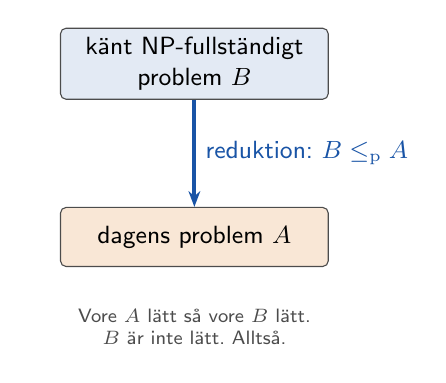
\begin{tikzpicture}
        \node[bx,fill=kthblue!12,minimum width=34mm] (B) at (0,2.2) {känt NP-fullständigt\\problem $B$};
        \node[bx,fill=warnorange!18,minimum width=34mm] (A) at (0,0) {dagens problem $A$};
        \draw[flow,line width=1.4pt,kthblue] (B) -- node[right,font=\small] {reduktion: $B\lep A$} (A);
        \node[lab,align=flush center,text width=40mm] at (0,-1.15) {Vore $A$ lätt så vore $B$ lätt.\\$B$ är inte lätt. Alltså.};
      \end{tikzpicture}
    \end{column}
  \end{columns}
\end{frame}

% ===================== del1-uppgifter.tex =====================
\section{Dagens uppgifter}

% ---------------------------------------------------------------- Uppgift 1
\newcommand{\uppgiftEtt}{%
  \begin{columns}[T]
    \begin{column}{0.61\textwidth}
      \small
      \textbf{Kappsäcksproblemet} (välkänt NP-fullständigt, föreläsning 21):
      \begin{itemize}
        \item \textbf{Indata:} en mängd $P$ av prylar med vikt $w_i$ och värde $v_i$, en kappsäcksstorlek $S$ och ett mål $K$. Alla tal är ickenegativa heltal.
        \item \textbf{Fråga:} går det att välja ut prylar av sammanlagt värde minst $K$ så att deras sammanlagda vikt är högst $S$?
      \end{itemize}
      Anta att vi har en algoritm $A$ som löser detta beslutsproblem.
      \begin{block}{Uppgift}
        \small Konstruera en algoritm som med samma indata som $A$ dels besvarar kappsäcksproblemet, dels -- om svaret är ja -- talar om precis \emph{vilka} prylar som ska packas. Den får anropa $A$ $O(|P|)$ gånger men får i övrigt inte ta mer än polynomisk tid.

        \smallskip
        Du konstruerar och analyserar alltså en \emph{turingreduktion} av det konstruktiva kappsäcksproblemet till beslutsproblemet.
      \end{block}
    \end{column}
    \begin{column}{0.37\textwidth}
      \centering
      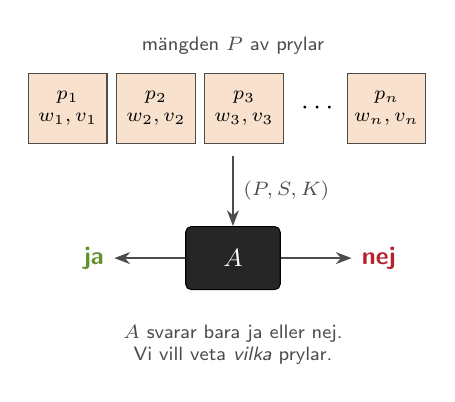
\begin{tikzpicture}
        \foreach \k/\lbl in {0/1,1/2,2/3} {
          \node[draw=black!70,fill=warnorange!22,minimum width=10mm,minimum height=9mm,font=\scriptsize,align=center,inner sep=1pt] at (\k*1.12,0) {$p_{\lbl}$\\$w_{\lbl},v_{\lbl}$};
        }
        \node at (3.2,0) {$\cdots$};
        \node[draw=black!70,fill=warnorange!22,minimum width=10mm,minimum height=9mm,font=\scriptsize,align=center,inner sep=1pt] at (4.05,0) {$p_{n}$\\$w_{n},v_{n}$};
        \node[lab] at (2.1,0.8) {mängden $P$ av prylar};
        \node[orakel] (A) at (2.1,-1.9) {$A$};
        \draw[flow] (2.1,-0.6) -- node[right,lab] {$(P,S,K)$} (A);
        \draw[flow] (A.west) -- ++(-0.9,0) node[left,font=\small] {\ja};
        \draw[flow] (A.east) -- ++(0.9,0) node[right,font=\small] {\nej};
        \node[lab,align=center] at (2.1,-3.0) {$A$ svarar bara ja eller nej.\\Vi vill veta \emph{vilka} prylar.};
      \end{tikzpicture}
    \end{column}
  \end{columns}
}
\begin{frame}{Uppgift 1: Konstruera kappsäckslösning}{uppgiften}
  \uppgiftEtt
\end{frame}

% ---------------------------------------------------------------- Uppgift 2
\newcommand{\uppgiftTva}{%
  \begin{columns}[T]
    \begin{column}{0.68\textwidth}
      \small
      \begin{itemize}
        \item Datorer och förbindelser går sönder. Man vill därför ha alternativa vägar mellan varje par av datorer.
        \item Finns tre vägar från $A$ till $B$ som är helt disjunkta (utom ändpunkterna) kan två datorer, vilka som helst, försvinna utan att $A$ och $B$ tappar kontakten.
        \item \textbf{Modell:} oriktad graf; hörn = datorer, kant $(X,Y)$ = \emph{möjlig} direktförbindelse.
        \item Tillförlitlighet $T(X,Y)$: antalet disjunkta vägar som ska finnas mellan $X$ och $Y$.
        \item Budget $B$: antalet direktförbindelser man har råd att bygga.
      \end{itemize}
      \begin{block}{Uppgift}
        \small Går det att plocka ut en delgraf bestående av $B$ kanter så att det för alla par av hörn $(X,Y)$ finns minst $T(X,Y)$ disjunkta stigar i delgrafen mellan $X$ och $Y$? Visa att detta problem är NP-fullständigt!
      \end{block}
    \end{column}
    \begin{column}{0.3\textwidth}
      \centering
      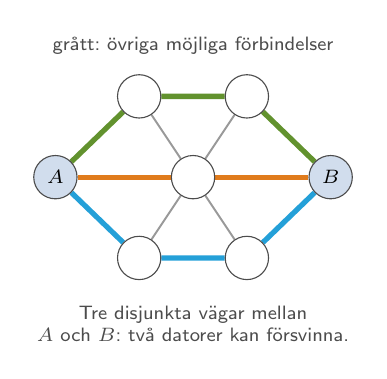
\begin{tikzpicture}[scale=0.76]
        \node[vx,fill=kthblue!20] (A) at (0,0) {$A$};
        \node[vx,fill=kthblue!20] (B) at (4.6,0) {$B$};
        \node[vx] (u1) at (1.4,1.35) {};
        \node[vx] (u2) at (3.2,1.35) {};
        \node[vx] (m) at (2.3,0) {};
        \node[vx] (d1) at (1.4,-1.35) {};
        \node[vx] (d2) at (3.2,-1.35) {};
        \begin{scope}[on background layer]
          \draw[ed] (u1) -- (m) -- (d2) (u2) -- (m) -- (d1);
          \draw[pA] (A) -- (u1) -- (u2) -- (B);
          \draw[pB] (A) -- (m) -- (B);
          \draw[pC] (A) -- (d1) -- (d2) -- (B);
        \end{scope}
        \node[lab,align=center] at (2.3,-2.45) {Tre disjunkta vägar mellan\\$A$ och $B$: två datorer kan försvinna.};
        \node[lab,align=center] at (2.3,2.2) {grått: övriga möjliga förbindelser};
      \end{tikzpicture}
    \end{column}
  \end{columns}
}
\begin{frame}{Uppgift 2: Tillförlitlighet hos Internet}{uppgiften}
  \uppgiftTva
\end{frame}

% ---------------------------------------------------------------- Uppgift 3
\newcommand{\uppgiftTre}{%
  \begin{columns}[T]
    \begin{column}{0.57\textwidth}
      \small
      \begin{itemize}
        \item Håstads leksaksaffär säljer ett pussel som består av en låda och ett antal kort.
        \item Ett kort kan placeras i lådan på två sätt, med framsidan upp eller med baksidan upp, eftersom det finns urgröpningar i korten som måste passa in i lister som sitter i lådan.
        \item På varje kort finns två kolumner med hål, men vissa av hålen är igenfyllda.
        \item \textbf{Mål:} lägg korten i lådan så att hela botten täcks -- för varje hålposition måste alltså åtminstone ett av korten ha ett igenfyllt hål.
      \end{itemize}
    \end{column}
    \begin{column}{0.41\textwidth}
      \centering
      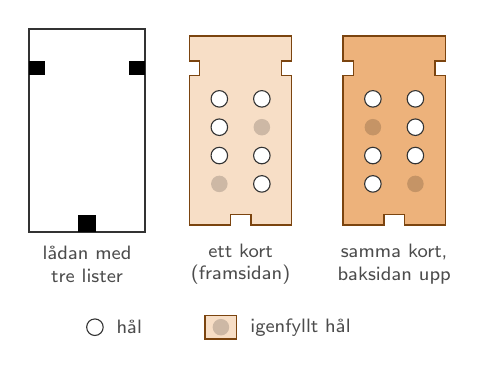
\begin{tikzpicture}[scale=1.0]
        % lådan med tre lister (kH = 2.40 för fyra rader)
        \draw[black!80,line width=0.8pt] (-0.09,-0.09) rectangle (1.39,2.49);
        \fill[black] (-0.09,1.905) rectangle (0.12,2.075);
        \fill[black] (1.18,1.905) rectangle (1.39,2.075);
        \fill[black] (0.535,-0.09) rectangle (0.765,0.12);
        \hkort{1.95}{0}{0,0,0,1}{0,1,0,0}{}{kort}
        \hkort{3.9}{0}{0,1,0,0}{0,0,0,1}{}{kortvand}
        \node[lab,align=center] at (0.65,-0.5) {lådan med\\tre lister};
        \node[lab,align=center] at (2.6,-0.5) {ett kort\\(framsidan)};
        \node[lab,align=center] at (4.55,-0.5) {samma kort,\\baksidan upp};
        \path[korthal] (0.75,-1.3) circle (0.105); \node[lab,right] at (0.9,-1.3) {hål};
        \path[kort] (2.15,-1.45) rectangle (2.55,-1.15); \path[fill=kortm] (2.35,-1.3) circle (0.105); \node[lab,right] at (2.6,-1.3) {igenfyllt hål};
      \end{tikzpicture}
    \end{column}
  \end{columns}
  \vspace{1mm}
  \begin{block}{Uppgift}
    \small Bevisa att språket\quad
    $\prob{Toys}=\{\langle c_1,c_2,\dots,c_n\rangle : (c_i$ beskriver kort$)\,\land\,($det går att lösa pusslet$)\}$\quad
    är NP-fullständigt.
  \end{block}
}
\begin{frame}{Uppgift 3: Håstads leksaksaffär}{uppgiften}
  \uppgiftTre
\end{frame}

% ---------------------------------------------------------------- Uppgift 4
\newcommand{\uppgiftFyra}{%
  \begin{columns}[T]
    \begin{column}{0.58\textwidth}
      \small
      \begin{itemize}
        \item Givet: $n$ jobb som ska exekveras och ett tillräckligt antal processorer.
        \item Varje jobb tar en tidsenhet att utföra.
        \item Det finns också villkor på formen \emph{jobb $i$ kan inte exekveras samtidigt som jobb $j$}.
        \item \prob{Schedule}: går det att schemalägga jobben så att alla jobb kan exekveras på tre tidsenheter?
      \end{itemize}
      \begin{block}{Uppgift}
        \begin{enumerate}
          \item[a)] Visa att \prob{Schedule} är NP-fullständigt.
          \item[b)] Är problemet fortfarande NP-fullständigt om vi kräver att jobben ska vara exekverade efter $k$ tidsenheter där $k>3$?
          \item[c)] Är det sant för $k=2$?
        \end{enumerate}
      \end{block}
    \end{column}
    \begin{column}{0.4\textwidth}
      \centering
      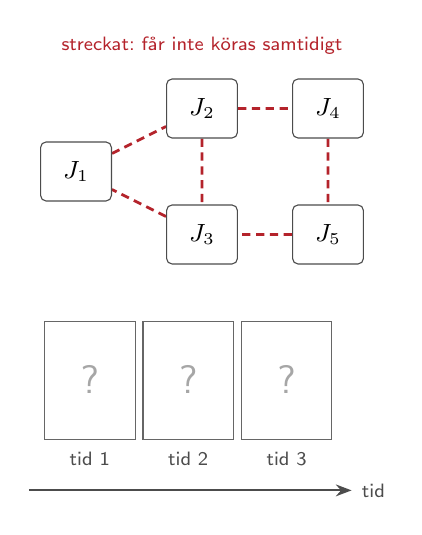
\begin{tikzpicture}
        \node[bx,minimum width=9mm] (j1) at (0,1.1) {$J_1$};
        \node[bx,minimum width=9mm] (j2) at (1.6,1.9) {$J_2$};
        \node[bx,minimum width=9mm] (j3) at (1.6,0.3) {$J_3$};
        \node[bx,minimum width=9mm] (j4) at (3.2,1.9) {$J_4$};
        \node[bx,minimum width=9mm] (j5) at (3.2,0.3) {$J_5$};
        \begin{scope}[on background layer]
          \draw[badred,line width=1pt,densely dashed] (j1) -- (j2) -- (j3) -- (j1) (j2) -- (j4) -- (j5) -- (j3);
        \end{scope}
        \node[lab,text=badred] at (1.6,2.7) {streckat: får inte köras samtidigt};
        % tre tomma tidsenheter
        \foreach \t in {1,2,3} {
          \draw[black!60] (\t*1.25-1.65,-2.3) rectangle (\t*1.25-0.5,-0.8);
          \node[lab] at (\t*1.25-1.075,-2.55) {tid \t};
          \node[text=black!35,font=\Large] at (\t*1.25-1.075,-1.55) {?};
        }
        \draw[flow] (-0.6,-2.95) -- (3.5,-2.95) node[right,lab] {tid};
      \end{tikzpicture}
    \end{column}
  \end{columns}
}
\begin{frame}{Uppgift 4: Processorschemaläggning}{uppgiften}
  \uppgiftFyra
\end{frame}

% ---------------------------------------------------------------- Uppgift 5
\newcommand{\uppgiftFem}{%
  \begin{columns}[T]
    \begin{column}{0.58\textwidth}
      \small
      \begin{itemize}
        \item \emph{Patchwork}, från programvaruföretaget Stitcher, pusslar ihop rektangulära lappar till ett lapptäcke utan hål och utan lappar som överlappar varandra.
        \item \textbf{Indata:} en lista av rektangulära lappar (bredd och höjd i hela millimeter) och önskad storlek (bredd och höjd) på det färdiga rektangulära lapptäcket.
        \item \textbf{Utdata:} om en \emph{delmängd} av lapparna kan pusslas ihop till ett täcke av rätt storlek -- en beskrivning av hur. För varje lapp som används: var den ska placeras och om den behöver vridas.
      \end{itemize}
      \begin{block}{Uppgift}
        \small Formulera detta konstruktionsoptimeringsproblem med matematisk notation och visa att det tillhörande beslutsproblemet (existerar en lösning?) är NP-fullständigt.
      \end{block}
    \end{column}
    \begin{column}{0.4\textwidth}
      \centering
      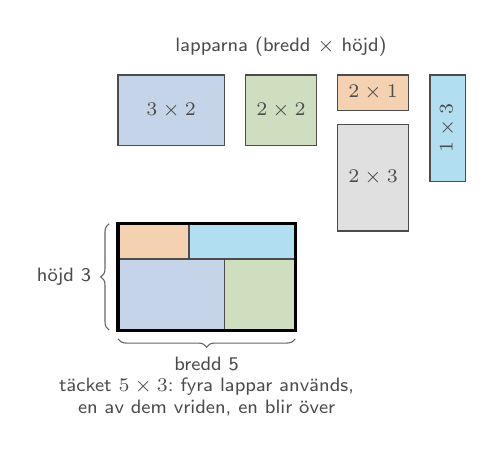
\begin{tikzpicture}[x=4.5mm,y=4.5mm]
        % lösa lappar
        \draw[lapp,fill=kthblue!25] (0,5.2) rectangle +(3,2); \node[lab] at (1.5,6.2) {$3\times2$};
        \draw[lapp,fill=okgreen!30] (3.6,5.2) rectangle +(2,2); \node[lab] at (4.6,6.2) {$2\times2$};
        \draw[lapp,fill=warnorange!35] (6.2,6.2) rectangle +(2,1); \node[lab] at (7.2,6.7) {$2\times1$};
        \draw[lapp,fill=kthsky!35] (8.8,4.2) rectangle +(1,3); \node[lab,rotate=90] at (9.3,5.7) {$1\times3$};
        \draw[lapp,fill=black!12] (6.2,2.8) rectangle +(2,3); \node[lab] at (7.2,4.3) {$2\times3$};
        \node[lab] at (4.6,8.0) {lapparna (bredd $\times$ höjd)};
        % täcket
        \draw[lapp,fill=kthblue!25] (0,0) rectangle +(3,2);
        \draw[lapp,fill=okgreen!30] (3,0) rectangle +(2,2);
        \draw[lapp,fill=warnorange!35] (0,2) rectangle +(2,1);
        \draw[lapp,fill=kthsky!35] (2,2) rectangle +(3,1);
        \draw[black,line width=1.1pt] (0,0) rectangle (5,3);
        \draw[decorate,decoration={brace,mirror,amplitude=3pt},black!60] (0,-0.25) -- (5,-0.25) node[midway,below=3pt,lab] {bredd 5};
        \draw[decorate,decoration={brace,amplitude=3pt},black!60] (-0.25,0) -- (-0.25,3) node[midway,left=3pt,lab] {höjd 3};
        \node[lab,align=center] at (2.5,-1.9) {täcket $5\times3$: fyra lappar används,\\en av dem vriden, en blir över};
      \end{tikzpicture}
    \end{column}
  \end{columns}
}
\begin{frame}{Uppgift 5: Lapptäcke}{uppgiften}
  \uppgiftFem
\end{frame}

% ---------------------------------------------------------------- Ledtrådar
\begin{frame}{Fastnat? En ledtråd per uppgift}
  \begin{columns}[T]
    \begin{column}{0.62\textwidth}
      Fundera en stund innan vi löser dem. Den som vill ha hjälp på traven:
      \begin{enumerate}
        \item<2-> \textbf{Kappsäck:} fråga $A$ vad som händer om en pryl försvinner.
        \item<3-> \textbf{Internet:} reducera \prob{Hamiltonsk krets} (Viggos egen ledning). Vilken budget och vilka $T$-värden tvingar fram en cykel?
        \item<4-> \textbf{Håstad:} ett kort kan ligga på två sätt. Vad mer i den här kursen kan anta precis två värden?
        \item<5-> \textbf{Schemaläggning:} rita jobben som hörn och konflikterna som kanter. Titta sedan länge på bilden.
        \item<6-> \textbf{Lapptäcke:} gör täcket en millimeter högt.
      \end{enumerate}
    \end{column}
    \begin{column}{0.36\textwidth}
      \onslide<7->{
      \begin{block}{Gemensamt för uppgift 2--5}
        Hitta ett \emph{känt} NP-fullständigt problem som liknar ditt, och visa att det kända problemet kan lösas med hjälp av ditt.

        \smallskip
        Det svåra är nästan aldrig beviset. Det svåra är att välja rätt kusin.
      \end{block}}
    \end{column}
  \end{columns}
\end{frame}

% ===================== del2-teori.tex =====================
\section{Verktygslådan}

\begin{frame}{Repetition: NP, NP-svårt, NP-fullständigt}
  \begin{columns}[T]
    \begin{column}{0.57\textwidth}
      \begin{itemize}
        \item<1-> \textbf{Beslutsproblem:} svaret är ja eller nej.
        \item<2-> \textbf{NP:} varje ja-instans har en lösning (ett \emph{certifikat}) som kan verifieras på polynomisk tid.
        \item<3-> \textbf{NP-svårt:} $A$ är NP-svårt om \emph{varje} problem i NP kan reduceras till $A$ på polynomisk tid.
        \item<4-> \textbf{NP-fullständigt:} $A\in\mathrm{NP}$ och $A$ är NP-svårt.
        \item<5-> De NP-fullständiga problemen är alltså de svåraste i NP. Löser du ett av dem på polynomisk tid har du löst alla, och visat att $\mathrm{P}=\mathrm{NP}$.
        \item<6-> Vi behöver aldrig reducera \emph{varje} problem i NP. Det räcker med \emph{ett} som redan är NP-svårt, eftersom reduktioner kan kedjas.
      \end{itemize}
    \end{column}
    \begin{column}{0.41\textwidth}
      \centering
      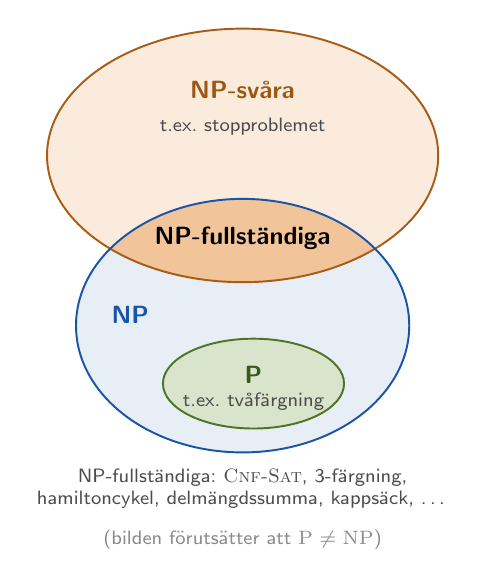
\begin{tikzpicture}[scale=0.92]
        \fill[warnorange!15] (0,2.35) ellipse (2.7 and 1.75);
        \fill[kthblue!10] (0,0) ellipse (2.3 and 1.75);
        \begin{scope}
          \clip (0,0) ellipse (2.3 and 1.75);
          \fill[warnorange!45] (0,2.35) ellipse (2.7 and 1.75);
        \end{scope}
        \draw[warnorange!75!black,line width=0.7pt] (0,2.35) ellipse (2.7 and 1.75);
        \draw[kthblue,line width=0.7pt] (0,0) ellipse (2.3 and 1.75);
        \draw[okgreen!80!black,fill=okgreen!25,line width=0.7pt] (0.15,-0.8) ellipse (1.25 and 0.62);
        \node[font=\small\bfseries,text=warnorange!70!black] at (0,3.25) {NP-svåra};
        \node[lab] at (0,2.75) {t.ex.\ stopproblemet};
        \node[font=\small\bfseries] at (0,1.2) {NP-fullständiga};
        \node[font=\small\bfseries,text=kthblue] at (-1.55,0.15) {NP};
        \node[font=\small\bfseries,text=okgreen!60!black] at (0.15,-0.68) {P};
        \node[lab] at (0.15,-1.05) {t.ex.\ tvåfärgning};
        \node[lab,align=center] at (0,-2.25) {NP-fullständiga: \prob{Cnf-Sat}, 3-färgning,\\hamiltoncykel, delmängdssumma, kappsäck, \dots};
        \node[lab,text=softgray] at (0,-2.95) {(bilden förutsätter att $\mathrm{P}\neq\mathrm{NP}$)};
      \end{tikzpicture}
    \end{column}
  \end{columns}
\end{frame}

\begin{frame}{Tre sorters problem}
  \centering
  \begin{tabular}{@{}L{3.9cm}L{7.0cm}L{1.9cm}@{}}
    \toprule
     & \textbf{Kappsäck som \dots} & \textbf{Svar} \\
    \midrule
    \textbf{Beslutsproblem} & Finns en packning med värde $\ge K$ och vikt $\le S$? & ja eller nej \\
    \textbf{Optimeringsproblem} & Vilket är det största värde som ryms i säcken? & ett tal \\
    \textbf{Konstruktionsproblem} & Vilka prylar ska packas? & en lösning \\
    \bottomrule
  \end{tabular}
  \vspace{3mm}
  \begin{itemize}
    \item<2-> NP och NP-fullständighet är definierade för \textbf{beslutsproblem}. Därför skriver vi om allt till ja/nej-frågor innan vi bevisar något.
    \item<3-> Den som kan konstruera en lösning kan förstås också svara ja eller nej. Åt det hållet är det gratis.
    \item<4-> \textbf{Uppgift 1} går åt andra hållet: från ja/nej-svar till en färdig packning.
    \item<5-> \textbf{Uppgift 5} ber oss först formulera ett konstruktionsproblem, och sedan bevisa att det tillhörande beslutsproblemet är NP-fullständigt.
  \end{itemize}
\end{frame}

\begin{frame}{Karpreduktion och turingreduktion}
  \begin{columns}[T]
    \begin{column}{0.5\textwidth}
      \begin{block}{Karpreduktion av $P$ till $Q$}
        En algoritm som löser $P$ med \emph{exakt ett} anrop till $Q$, och där svaret från anropet returneras direkt. Allt annat arbete tar polynomisk tid.
      \end{block}
      \onslide<2->{
      \begin{block}{Turingreduktion av $P$ till $Q$}
        En algoritm som löser $P$ genom att anropa $Q$ en eller flera gånger. Allt annat arbete tar polynomisk tid.
      \end{block}}
      \onslide<3->{
      \begin{alertblock}{Observera!}
        I ett NP-svårighetsbevis måste reduktionen vara en \textbf{karpreduktion}.
      \end{alertblock}}
    \end{column}
    \begin{column}{0.48\textwidth}
      \centering
      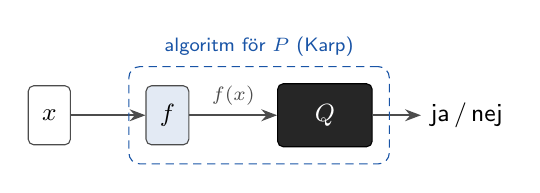
\begin{tikzpicture}
        \node[bx] (x) at (0,0) {$x$};
        \node[bx,fill=kthblue!12] (f) at (1.5,0) {$f$};
        \node[orakel] (Q) at (3.5,0) {$Q$};
        \node[font=\small] (ans) at (5.3,0) {ja\,/\,nej};
        \draw[flow] (x) -- (f);
        \draw[flow] (f) -- node[above,lab] {$f(x)$} (Q);
        \draw[flow] (Q) -- (ans);
        \node[draw=kthblue,densely dashed,rounded corners,fit=(f)(Q),inner sep=6pt] (boxK) {};
        \node[lab,text=kthblue,above=0pt of boxK] {algoritm för $P$ (Karp)};
      \end{tikzpicture}

      \vspace{3mm}
      \onslide<2->{%
      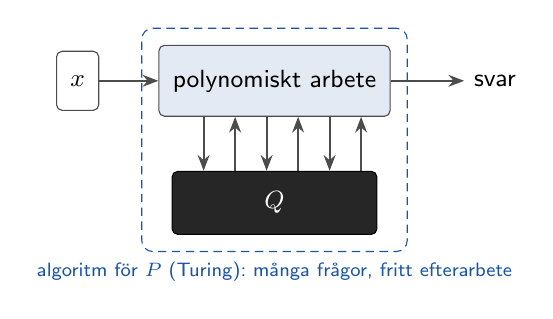
\begin{tikzpicture}
        \node[bx] (x) at (0,0) {$x$};
        \node[bx,fill=kthblue!12,minimum width=26mm,minimum height=9mm] (alg) at (2.5,0) {polynomiskt arbete};
        \node[orakel,minimum width=26mm] (Q) at (2.5,-1.55) {$Q$};
        \node[font=\small] (ans) at (5.3,0) {svar};
        \draw[flow] (x) -- (alg);
        \draw[flow] (alg) -- (ans);
        \foreach \dx in {-9,-1,7} \draw[flow] ([xshift=\dx mm]alg.south) -- ([xshift=\dx mm]Q.north);
        \foreach \dx in {-5,3,11} \draw[flow] ([xshift=\dx mm]Q.north) -- ([xshift=\dx mm]alg.south);
        \node[draw=kthblue,densely dashed,rounded corners,fit=(alg)(Q),inner sep=6pt] (boxT) {};
        \node[lab,text=kthblue,below=0pt of boxT] {algoritm för $P$ (Turing): många frågor, fritt efterarbete};
      \end{tikzpicture}}
    \end{column}
  \end{columns}
\end{frame}

\begin{frame}{\rabbit varför duger inte en turingreduktion i ett NP-svårighetsbevis?}
  \begin{itemize}
    \item<1-> Med en turingreduktion får man göra vad man vill med svaren. Till exempel negera dem.
    \item<2-> Då kan \prob{Osatisfierbarhet} (''saknar formeln lösning?'') reduceras till \prob{Sat}: ett anrop, en negation, klart.
    \item<3-> Men ingen vet hur ett kort certifikat för att en formel \emph{saknar} lösning skulle se ut. Det är frågan om $\mathrm{NP}=\mathrm{co\text{-}NP}$, och de flesta tror att svaret är nej.
    \item<4-> Karpreduktioner bevarar däremot strukturen ''ja-instanser har certifikat'':
      \[A\lep B \ \text{ och }\ B\in\mathrm{NP} \quad\Longrightarrow\quad A\in\mathrm{NP}.\]
      Certifikatet för $f(x)$ fungerar som certifikat för $x$.
    \item<5-> För konstruktions- och optimeringsproblem finns inget ja/nej-svar att skicka vidare. Där är turingreduktioner det naturliga verktyget -- som i uppgift 1.
  \end{itemize}
\end{frame}

\begin{frame}{Reduktionens riktning}
  \begin{columns}[T]
    \begin{column}{0.55\textwidth}
      \begin{itemize}
        \item<1-> Vi vill visa att \emph{vårt} problem $A$ är svårt.
        \item<2-> Då ska ett \emph{känt} svårt problem $B$ reduceras \emph{till} $A$:\quad $B\lep A$.
        \item<3-> Läs $B\lep A$ som ''$B$ är inte svårare än $A$''. En snabb algoritm för $A$ skulle ge en snabb algoritm för $B$.
        \item<4-> I den här kursen skriver vi reduktionen som en algoritm: \emph{lös det kända problemet med hjälp av ditt eget.}
        \item<5-> \textbf{Fel håll} ($A\lep B$) visar bara att $A$ inte är svårare än $B$. Att reducera sitt problem till \prob{Sat} bevisar mest att \prob{Sat}-lösare är användbara.
      \end{itemize}
    \end{column}
    \begin{column}{0.43\textwidth}
      \centering
      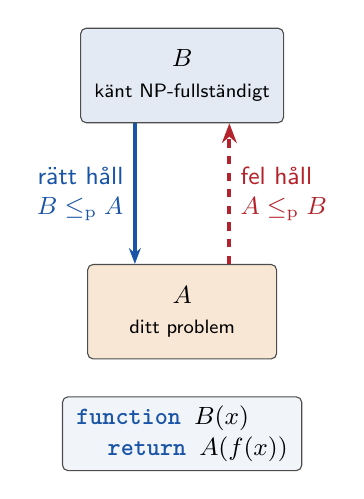
\begin{tikzpicture}
        \node[bx,fill=kthblue!12,minimum width=24mm,minimum height=12mm] (B) at (0,0) {$B$\\{\scriptsize känt NP-fullständigt}};
        \node[bx,fill=warnorange!18,minimum width=24mm,minimum height=12mm] (A) at (0,-3.0) {$A$\\{\scriptsize ditt problem}};
        \draw[flow,line width=1.6pt,kthblue,visible on=<2->] ([xshift=-6mm]B.south) -- node[left,font=\small,text=kthblue,align=right] {rätt håll\\$B\lep A$} ([xshift=-6mm]A.north);
        \draw[bad,visible on=<5->] ([xshift=6mm]A.north) -- node[right,font=\small,text=badred,align=left] {fel håll\\$A\lep B$} ([xshift=6mm]B.south);
        \node[bx,align=left,font=\ttfamily\small,fill=kthblue!6,visible on=<4->] at (0,-4.55) {\textcolor{kthblue}{\textbf{function}} $B(x)$\\\hspace*{1.2em}\textcolor{kthblue}{\textbf{return}} $A(f(x))$};
      \end{tikzpicture}
    \end{column}
  \end{columns}
\end{frame}

\begin{frame}{Receptet: så bevisar man att $A$ är NP-fullständigt}
  \begin{columns}[T]
    \begin{column}{0.46\textwidth}
      \begin{block}{1. Visa att $A\in\mathrm{NP}$}
        \begin{enumerate}
          \item[a)] Föreslå vad en lösning (ett certifikat) är.
          \item[b)] Visa hur lösningen verifieras.
          \item[c)] Visa att verifikationen tar polynomisk tid i indatas storlek.
        \end{enumerate}
      \end{block}
    \end{column}
    \begin{column}{0.52\textwidth}
      \onslide<2->{
      \begin{block}{2. Visa att $A$ är NP-svårt}
        \begin{enumerate}
          \item[a)] Välj ett känt NP-fullständigt problem $B$.
          \item[b)] Beskriv en karpreduktion av $B$ till $A$.
          \item[c)] Visa att reduktionen tar polynomisk tid.
          \item[d)] Visa att den är korrekt: ja-instanser blir ja-instanser och nej-instanser blir nej-instanser.
        \end{enumerate}
      \end{block}}
    \end{column}
  \end{columns}
  \vspace{2mm}
  \begin{itemize}
    \item<3-> Steg 2d är i praktiken två implikationer: ''$x$ ja $\Rightarrow f(x)$ ja'' och ''$f(x)$ ja $\Rightarrow x$ ja''. Den andra är nej-till-nej skriven baklänges, och det är oftast där det intressanta händer.
    \item<4-> Alla fyra NP-fullständighetsbevisen i dag följer mallen till punkt och pricka. Det är en egenskap hos bevisen, inte en brist på fantasi.
  \end{itemize}
\end{frame}

\begin{frame}[fragile]{Indatas storlek mäts i bitar}
  \prob{Delmängdssumma}: har någon delmängd av heltalen $p_1,\dots,p_n>0$ summan exakt $K$?
  \begin{columns}[T]
    \begin{column}{0.52\textwidth}
\begin{lstlisting}
function DelmängdssummaDP($p_1, \dots, p_n$, K)
    nås[0] <- ja;  nås[1..K] <- nej
    for i <- 1 to n do
        for s <- K downto $p_i$ do
            if nås[s - $p_i$] then nås[s] <- ja
    return nås[K]
\end{lstlisting}
      \begin{itemize}
        \item<2-> Med enhetskostnad: $O(n\cdot K)$. Polynomiskt?
        \item<3-> $K$ står i indata med $b\approx\log_2 K$ bitar. Uttryckt i $b$ är tiden $O(n\cdot 2^b)$.
        \item<4-> En algoritm som är polynomisk i \emph{talvärdena} i indata men exponentiell i indatas \emph{längd} kallas \textbf{pseudopolynomisk}.
      \end{itemize}
    \end{column}
    \begin{column}{0.46\textwidth}
      \centering
      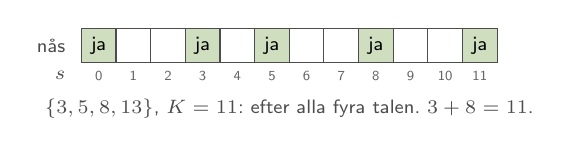
\begin{tikzpicture}
        \foreach \s/\v in {0/1,1/0,2/0,3/1,4/0,5/1,6/0,7/0,8/1,9/0,10/0,11/1} {
          \ifnum\v=1
            \node[smallcell,hlok,minimum size=4.4mm] at (\s*0.44,0) {ja};
          \else
            \node[smallcell,minimum size=4.4mm] at (\s*0.44,0) {};
          \fi
          \node[font=\tiny,text=black!60] at (\s*0.44,-0.38) {\s};
        }
        \node[lab,anchor=east] at (-0.3,0) {nås};
        \node[lab,anchor=east] at (-0.3,-0.38) {$s$};
        \node[lab] at (2.42,-0.8) {$\{3,5,8,13\}$, $K=11$: efter alla fyra talen. $3+8=11$.};
      \end{tikzpicture}

      \vspace{1mm}
      \onslide<3->{\small\setlength{\tabcolsep}{4pt}%
      \begin{tabular}{@{}rrrl@{}}
        \toprule
        $K$ & bitar & rutor & vid $10^9$ rutor/s\\
        \midrule
        $255$ & 8 & $256$ & omärkligt\\
        $\approx 10^{6}$ & 20 & $10^{6}$ & 1 ms\\
        $\approx 10^{18}$ & 60 & $10^{18}$ & 32 år\\
        $\approx 3\cdot10^{38}$ & 128 & $3\cdot10^{38}$ & $10^{22}$ år\\
        \bottomrule
      \end{tabular}

      \vspace{1mm}
      {\scriptsize (tid för ett varv i den yttre slingan, alltså per tal $p_i$)}}

      \vspace{1mm}
      \onslide<5->{{\raggedright\small\rabbit går det att vara smartare? Inte såvitt någon vet. \prob{Delmängdssumma} är NP-fullständigt: en polynomisk algoritm vore ett bevis för $\mathrm{P}=\mathrm{NP}$.\par}}
    \end{column}
  \end{columns}
\end{frame}

\begin{frame}[fragile]{Fyra sätt att mäta samma algoritm}
  \begin{columns}[T]
    \begin{column}{0.49\textwidth}
\begin{lstlisting}
function ArithmeticSum(N)
    s <- 0
    for i <- 1 to N do
        s <- s + i
    return s
\end{lstlisting}
      \centering\small
      \begin{tabular}{@{}lcc@{}}
        \toprule
         & enhetskostnad & bitkostnad\\
        \midrule
        mätt i $N$ & $O(N)$ & $O(N\log N)$\\
        mätt i $m=\log N$ & $O(2^m)$ & $O(m\,2^m)$\\
        \bottomrule
      \end{tabular}

      \vspace{1mm}
      {\raggedright\textcolor{badred}{Pseudopolynomisk:} ser bara polynomisk ut.\par}
    \end{column}
    \begin{column}{0.49\textwidth}
      \begin{visibleenv}<2->
\begin{lstlisting}
function SmartArithmeticSum(N)
    return N $\cdot$ (N+1) / 2
\end{lstlisting}
      \vspace{9.2mm}
      \centering\small
      \begin{tabular}{@{}lcc@{}}
        \toprule
         & enhetskostnad & bitkostnad\\
        \midrule
        mätt i $N$ & $O(1)$ & $O(\log^2 N)$\\
        mätt i $m=\log N$ & $O(1)$ & $O(m^2)$\\
        \bottomrule
      \end{tabular}

      \vspace{1mm}
      \textcolor{okgreen}{Polynomisk på riktigt.}
      \end{visibleenv}
    \end{column}
  \end{columns}
  \vspace{2mm}
  \begin{itemize}
    \item<3-> Bitkostnad: addition av $m$-bitstal kostar $O(m)$, multiplikation och division räknar vi som $O(m^2)$.
    \item<4-> Det som avgör är den nedre raden: tiden som funktion av \emph{antalet bitar} $m$.
    \item<5-> Pseudopolynomisk är en egenskap hos \emph{algoritmen}, inte hos problemet. Summan gick att räkna ut smartare. För \prob{Delmängdssumma} tror ingen att det går.
  \end{itemize}
\end{frame}

\begin{frame}{\rabbit varför just bitar?}
  \begin{columns}[T]
    \begin{column}{0.6\textwidth}
      \begin{itemize}
        \item<1-> NP är definierad med turingmaskiner. Indata är en rad tecken på ett band.
        \item<2-> Maskinen vet inte att tecknen ''betyder'' ett tal. Det enda den kan mäta sin tid mot är hur långt bandet är.
        \item<3-> Alltså: polynomisk tid betyder polynomisk i \emph{antalet bitar} i indata.
        \item<4-> Den som vill fuska kan skriva talen unärt ($5 = 11111$). Då blir indata långt och allting ser polynomiskt ut. Därför är binär kodning underförstådd.
        \item<5-> \textbf{Konsekvens i dag:} verifikationer och reduktioner måste vara polynomiska i antalet bitar. En slinga som går $S$ varv, eller en matris med $B\cdot H$ rutor, är inte det.
      \end{itemize}
    \end{column}
    \begin{column}{0.38\textwidth}
      \centering
      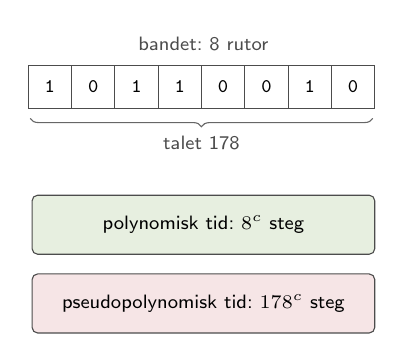
\begin{tikzpicture}
        % ett band
        \foreach \c [count=\i] in {1,0,1,1,0,0,1,0} {
          \node[cell,minimum size=5.5mm,font=\scriptsize\ttfamily] (c\i) at (\i*0.55,0) {\c};
        }
        \node[lab] at (2.5,0.55) {bandet: 8 rutor};
        \draw[decorate,decoration={brace,mirror,amplitude=3pt},black!60] (0.3,-0.4) -- (4.65,-0.4) node[midway,below=3pt,lab] {talet 178};
        \onslide<3->{
        \node[bx,fill=okgreen!15,text width=40mm,font=\scriptsize] at (2.5,-1.75) {polynomisk tid: $8^c$ steg};
        \node[bx,fill=badred!12,text width=40mm,font=\scriptsize] at (2.5,-2.75) {pseudopolynomisk tid: $178^c$ steg};}
      \end{tikzpicture}
      \onslide<5->{

      \vspace{2mm}
      {\small Vi kommer att möta bägge fallgroparna: kappsäck (uppgift 1) och lapptäcke (uppgift 5).}}
    \end{column}
  \end{columns}
\end{frame}

\begin{frame}{Dagens meny: kända NP-fullständiga problem}
  \begin{columns}[T]
    \begin{column}{0.18\textwidth}
      \centering\textbf{\small\prob{Cnf-Sat}}\\[1mm]
      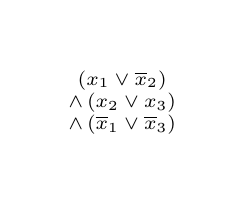
\begin{tikzpicture}
        \node[font=\scriptsize,align=center] at (0,0) {$(x_1\lor\xbar{2})$\\$\land\,(x_2\lor x_3)$\\$\land\,(\xbar{1}\lor\xbar{3})$};
        \path (-1.2,-0.95) rectangle (1.2,0.95);
      \end{tikzpicture}\\[1mm]
      {\scriptsize Kan variablerna ges värden så att varje klausul blir sann?\par}
    \end{column}
    \begin{column}{0.18\textwidth}
      \centering\textbf{\small 3-färgning}\\[1mm]
      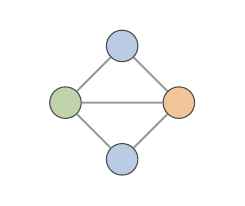
\begin{tikzpicture}[scale=0.8]
        \node[vx,t1,minimum size=4mm] (a) at (0,0.9) {};
        \node[vx,t2,minimum size=4mm] (b) at (-0.9,0) {};
        \node[vx,t3,minimum size=4mm] (c) at (0.9,0) {};
        \node[vx,t1,minimum size=4mm] (d) at (0,-0.9) {};
        \begin{scope}[on background layer]\draw[ed] (a) -- (b) -- (c) -- (a) (b) -- (d) -- (c);\end{scope}
        \path (-1.5,-1.19) rectangle (1.5,1.19);
      \end{tikzpicture}\\[1mm]
      {\scriptsize Kan hörnen färgas med tre färger så att grannar alltid får olika färg?\par}
    \end{column}
    \begin{column}{0.18\textwidth}
      \centering\textbf{\small Hamiltoncykel}\\[1mm]
      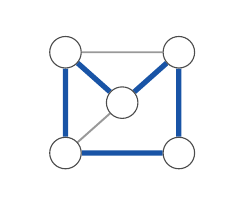
\begin{tikzpicture}[scale=0.8]
        \node[vx,minimum size=4mm] (a) at (-0.9,0.8) {};
        \node[vx,minimum size=4mm] (b) at (0.9,0.8) {};
        \node[vx,minimum size=4mm] (c) at (0.9,-0.8) {};
        \node[vx,minimum size=4mm] (d) at (-0.9,-0.8) {};
        \node[vx,minimum size=4mm] (e) at (0,0) {};
        \begin{scope}[on background layer]
          \draw[ed] (a) -- (b) (d) -- (e);
          \draw[sel] (a) -- (e) -- (b) -- (c) -- (d) -- (a);
        \end{scope}
        \path (-1.5,-1.19) rectangle (1.5,1.19);
      \end{tikzpicture}\\[1mm]
      {\scriptsize Finns en cykel som passerar varje hörn exakt en gång?\par}
    \end{column}
    \begin{column}{0.21\textwidth}
      \centering\textbf{\small Delmängdssumma}\\[1mm]
      \begin{tikzpicture}
        \node[font=\scriptsize,align=center] at (0,0) {$\{\textcolor{kthblue}{\mathbf 3},\,5,\,\textcolor{kthblue}{\mathbf 8},\,13\}$\\[2pt]$K=11$};
        \path (-1.2,-0.95) rectangle (1.2,0.95);
      \end{tikzpicture}\\[1mm]
      {\scriptsize Finns en delmängd av de positiva heltalen $p_1,\dots,p_n$ vars summa är exakt $K$?\par}
    \end{column}
    \begin{column}{0.18\textwidth}
      \centering\textbf{\small Kappsäck}\\[1mm]
      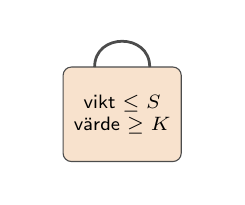
\begin{tikzpicture}
        \draw[black!70,fill=warnorange!22,rounded corners=3pt] (-0.75,-0.75) rectangle (0.75,0.45);
        \draw[black!70,line width=1pt] (-0.35,0.45) to[out=90,in=90,looseness=1.6] (0.35,0.45);
        \node[font=\scriptsize,align=center] at (0,-0.15) {vikt $\le S$\\värde $\ge K$};
        \path (-1.2,-0.95) rectangle (1.2,0.95);
      \end{tikzpicture}\\[1mm]
      {\scriptsize Finns prylar med sammanlagd vikt högst $S$ och sammanlagt värde minst $K$?\par}
    \end{column}
  \end{columns}
  \vspace{4mm}
  \begin{itemize}
    \item<2-> Alla fem är kända NP-fullständiga problem från föreläsningarna och får användas utan bevis.
    \item<3-> Fyra av dem blir utgångspunkt för var sitt bevis i dag. Den femte är redan huvudperson i uppgift 1.
  \end{itemize}
\end{frame}

% ===================== del3-kappsack.tex =====================
\section{Uppgift 1: Konstruera kappsäckslösning}

\begin{frame}{Uppgift 1: Konstruera kappsäckslösning}{uppgiften i repris}
  \uppgiftEtt
\end{frame}

\begin{frame}{Idén: fråga om en pryl i taget}{Uppgift 1}
  \begin{columns}[T]
    \begin{column}{0.58\textwidth}
      \begin{itemize}
        \item<1-> $A(P,S,K)$ säger bara om det finns \emph{någon} lösning. En instans kan ha noll, en eller flera.
        \item<2-> Fråga i stället $A$ om en mindre instans: $A(P-\{p\},S,K)$.
          \begin{itemize}
            \item<3-> \ja: det går att lösa problemet utan $p$. Släng $p$.
            \item<4-> \nej: det går \emph{inte} att lösa problemet utan $p$. Behåll $p$.
          \end{itemize}
        \item<5-> Gör så med varje pryl, en i taget. Det som är kvar när alla är prövade är en lösning.
        \item<6-> Samma idé med andra ord (Lisa Li, 2019): låtsas i tur och ordning att prylen $p$ har oändligt stor vikt. Svarar $A$ nej måste $p$ vara med.
      \end{itemize}
    \end{column}
    \begin{column}{0.4\textwidth}
      \centering
      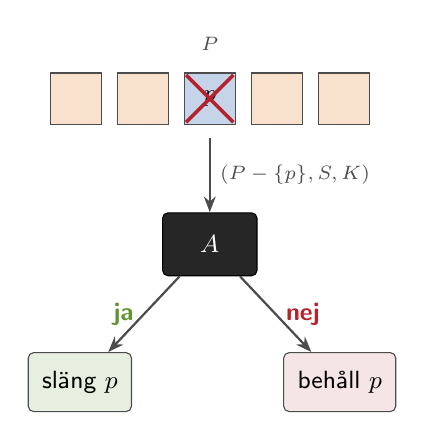
\begin{tikzpicture}
        \foreach \k in {1,2,4,5} \node[draw=black!70,fill=warnorange!22,minimum size=6.5mm] (q\k) at (\k*0.85,0) {};
        \node[draw=black!70,fill=kthblue!25,minimum size=6.5mm,font=\small] (q3) at (2.55,0) {$p$};
        \draw[badred,line width=1.3pt,visible on=<2->] (2.25,-0.3) -- (2.85,0.3) (2.25,0.3) -- (2.85,-0.3);
        \node[lab] at (2.55,0.7) {$P$};
        \node[orakel,visible on=<2->] (A) at (2.55,-1.85) {$A$};
        \draw[flow,visible on=<2->] (2.55,-0.5) -- node[right,lab] {$(P-\{p\},S,K)$} (A);
        \node[bx,fill=okgreen!15,visible on=<3->] (ja) at (0.9,-3.6) {släng $p$};
        \node[bx,fill=badred!12,visible on=<4->] (nej) at (4.2,-3.6) {behåll $p$};
        \draw[flow,visible on=<3->] (A) -- node[left,font=\small] {\ja} (ja);
        \draw[flow,visible on=<4->] (A) -- node[right,font=\small] {\nej} (nej);
      \end{tikzpicture}
    \end{column}
  \end{columns}
\end{frame}

\begin{frame}[fragile]{Algoritmen}{Uppgift 1}
\begin{lstlisting}
function Kappsäck(P, S, K)
    if not A(P, S, K) then return "Ingen lösning"
    foreach p in P do
        if A(P - {p}, S, K) then P <- P - {p}
    return P
\end{lstlisting}
  \begin{itemize}
    \item<2-> Slingan går över de \emph{ursprungliga} prylarna, en gång var. Mängden $P$ krymper under tiden.
    \item<3-> Antal anrop till $A$: ett före slingan och ett per pryl, alltså högst $|P|+1\in O(|P|)$.
    \item<4-> Allt övrigt arbete är mängdoperationer och tar polynomisk tid.
    \item<5-> Återstår att visa: mängden som returneras är verkligen en lösning -- inte bara något som \emph{innehåller} en lösning.
  \end{itemize}
\end{frame}

\begin{frame}{Exempel: sex prylar, $S=10$, $K=15$}{Uppgift 1}
  \centering
  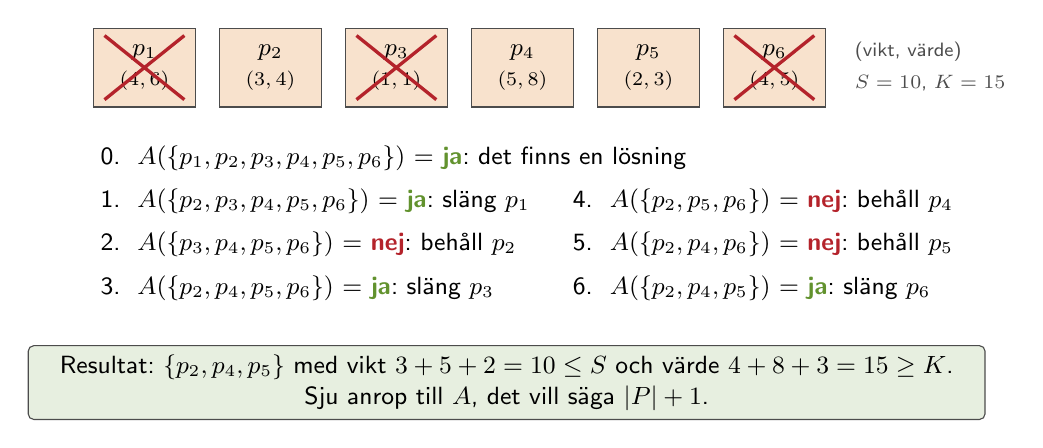
\begin{tikzpicture}
    % prylarna: (vikt, värde)
    \tikzset{pryl/.style={draw=black!70,fill=warnorange!22,minimum width=13mm,minimum height=10mm,font=\small,align=center,inner sep=1pt}}
    \node[pryl,alt=<3>{hl}{},alt=<4->{fill=black!8,text=black!40}{}] (p1) at (0,0) {$p_1$\\{\scriptsize $(4,6)$}};
    \node[pryl,alt=<4>{hl}{},alt=<5->{hlok}{}] (p2) at (1.6,0) {$p_2$\\{\scriptsize $(3,4)$}};
    \node[pryl,alt=<5>{hl}{},alt=<6->{fill=black!8,text=black!40}{}] (p3) at (3.2,0) {$p_3$\\{\scriptsize $(1,1)$}};
    \node[pryl,alt=<6>{hl}{},alt=<7->{hlok}{}] (p4) at (4.8,0) {$p_4$\\{\scriptsize $(5,8)$}};
    \node[pryl,alt=<7>{hl}{},alt=<8->{hlok}{}] (p5) at (6.4,0) {$p_5$\\{\scriptsize $(2,3)$}};
    \node[pryl,alt=<8>{hl}{},alt=<9->{fill=black!8,text=black!40}{}] (p6) at (8.0,0) {$p_6$\\{\scriptsize $(4,5)$}};
    \draw[badred,line width=1.2pt,visible on=<4->] ($(p1.south west)+(1.5mm,1mm)$) -- ($(p1.north east)+(-1.5mm,-1mm)$) ($(p1.north west)+(1.5mm,-1mm)$) -- ($(p1.south east)+(-1.5mm,1mm)$);
    \draw[badred,line width=1.2pt,visible on=<6->] ($(p3.south west)+(1.5mm,1mm)$) -- ($(p3.north east)+(-1.5mm,-1mm)$) ($(p3.north west)+(1.5mm,-1mm)$) -- ($(p3.south east)+(-1.5mm,1mm)$);
    \draw[badred,line width=1.2pt,visible on=<9->] ($(p6.south west)+(1.5mm,1mm)$) -- ($(p6.north east)+(-1.5mm,-1mm)$) ($(p6.north west)+(1.5mm,-1mm)$) -- ($(p6.south east)+(-1.5mm,1mm)$);
    \node[lab,anchor=west] at (8.9,0.2) {(vikt, värde)};
    \node[lab,anchor=west] at (8.9,-0.2) {$S=10$,\ $K=15$};
    % logg
    \tikzset{logg/.style={font=\small,anchor=west,inner sep=1pt}}
    \node[logg,visible on=<2->] at (-0.6,-1.15) {0.\ \ $A(\{p_1,p_2,p_3,p_4,p_5,p_6\})$ = \ja: det finns en lösning};
    \node[logg,visible on=<3->] at (-0.6,-1.70) {1.\ \ $A(\{p_2,p_3,p_4,p_5,p_6\})$ = \ja: släng $p_1$};
    \node[logg,visible on=<4->] at (-0.6,-2.25) {2.\ \ $A(\{p_3,p_4,p_5,p_6\})$ = \nej: behåll $p_2$};
    \node[logg,visible on=<5->] at (-0.6,-2.80) {3.\ \ $A(\{p_2,p_4,p_5,p_6\})$ = \ja: släng $p_3$};
    \node[logg,visible on=<6->] at (5.4,-1.70) {4.\ \ $A(\{p_2,p_5,p_6\})$ = \nej: behåll $p_4$};
    \node[logg,visible on=<7->] at (5.4,-2.25) {5.\ \ $A(\{p_2,p_4,p_6\})$ = \nej: behåll $p_5$};
    \node[logg,visible on=<8->] at (5.4,-2.80) {6.\ \ $A(\{p_2,p_4,p_5\})$ = \ja: släng $p_6$};
    \node[bx,fill=okgreen!15,text width=118mm,visible on=<9->] at (4.6,-4.0) {Resultat: $\{p_2,p_4,p_5\}$ med vikt $3+5+2=10\le S$ och värde $4+8+3=15\ge K$.\\ Sju anrop till $A$, det vill säga \mbox{$|P|+1$}.};
  \end{tikzpicture}
\end{frame}

\begin{frame}{Korrekthet, del 1: slingans invariant}{Uppgift 1}
  \begin{block}{Invariant}
    $A(P,S,K)$ = ja. Med andra ord: den aktuella mängden $P$ innehåller minst en lösning.
  \end{block}
  \begin{itemize}
    \item<2-> \textbf{Före slingan:} första raden har just kontrollerat det. Annars hade vi redan returnerat ''Ingen lösning''.
    \item<3-> \textbf{Ett varv:} $P$ ändras bara när $A(P-\{p\},S,K)$ = ja, och då innehåller också det nya $P$ en lösning.
    \item<4-> \textbf{Efter slingan:} mängden vi returnerar, $P_{\text{slut}}$, innehåller en lösning $Q\subseteq P_{\text{slut}}$.
    \item<5-> Det räcker inte riktigt. Vi lovade att $P_{\text{slut}}$ \emph{är} en lösning. Kan det ligga skräp kvar bredvid $Q$?
    \item<6-> Facit: nej, för slingan prövar varje pryl och plockar bort de överflödiga. Nästa bild skriver ut det argumentet i detalj.
  \end{itemize}
\end{frame}

\begin{frame}{Korrekthet, del 2: inget överflödigt blir kvar}{Uppgift 1}
  \begin{columns}[T]
    \begin{column}{0.6\textwidth}
      \textbf{Påstående:} $Q=P_{\text{slut}}$.
      \begin{itemize}
        \item<2-> Anta motsatsen: det finns en pryl $p\in P_{\text{slut}}$ som inte ligger i $Q$.
        \item<3-> När $p$ prövades var mängden $P'\supseteq P_{\text{slut}}$, för vi tar bara bort prylar.
        \item<4-> $p$ fick vara kvar, så $A(P'-\{p\},S,K)$ = nej.
        \item<5-> Men $Q\subseteq P_{\text{slut}}-\{p\}\subseteq P'-\{p\}$, och $Q$ är en lösning. Svaret borde ha varit ja. Motsägelse.
        \item<6-> Alltså är $P_{\text{slut}}$ själv en lösning: vikt högst $S$, värde minst $K$. \hfill$\Box$
      \end{itemize}
      \onslide<7->{\vspace{1mm}\rabbit varför räcker \emph{ett} varv? För att mängden bara krymper. En pryl som var nödvändig när den prövades förblir nödvändig i varje mindre mängd.}
    \end{column}
    \begin{column}{0.38\textwidth}
      \centering
      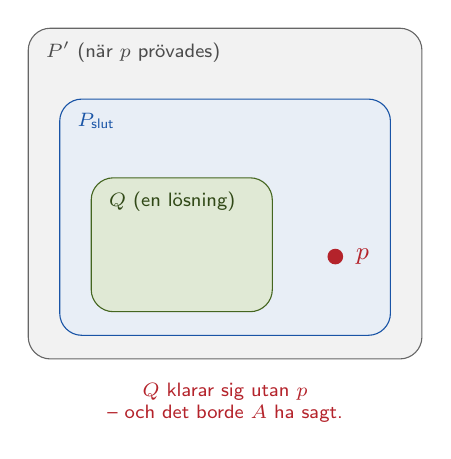
\begin{tikzpicture}
        \draw[black!60,fill=black!5,rounded corners=8pt] (0,0) rectangle (5.0,4.2);
        \node[lab,anchor=north west] at (0.1,4.15) {$P'$ (när $p$ prövades)};
        \draw[kthblue,fill=kthblue!10,rounded corners=8pt] (0.4,0.3) rectangle (4.6,3.3);
        \node[lab,text=kthblue,anchor=north west] at (0.5,3.25) {$P_{\text{slut}}$};
        \draw[okgreen!70!black,fill=okgreen!20,rounded corners=8pt,visible on=<2->] (0.8,0.6) rectangle (3.1,2.3);
        \node[lab,text=okgreen!50!black,anchor=north west,visible on=<2->] at (0.9,2.25) {$Q$ (en lösning)};
        \node[circle,fill=badred,inner sep=2pt,visible on=<2->] (p) at (3.9,1.3) {};
        \node[font=\small,text=badred,right=1pt of p,visible on=<2->] {$p$};
        \node[lab,text=badred,align=center,visible on=<5->] at (2.5,-0.55) {$Q$ klarar sig utan $p$\\-- och det borde $A$ ha sagt.};
      \end{tikzpicture}
    \end{column}
  \end{columns}
\end{frame}

\begin{frame}{Analys: vad har vi visat?}{Uppgift 1}
  \begin{columns}[T]
    \begin{column}{0.56\textwidth}
      \begin{itemize}
        \item<1-> Högst $|P|+1$ anrop till $A$, vart och ett på en instans som inte är större än den ursprungliga.
        \item<2-> Övrigt arbete: $O(|P|)$ mängdoperationer, polynomisk tid.
        \item<3-> Om beslutsproblemet går att lösa på tid $T(n)$ för indata av storlek $n$ går konstruktionsproblemet alltså på tid $O(n\cdot T(n))$ plus polynomiskt småplock.
        \item<4-> \textbf{Slutsats:} att konstruera en packning är inte svårare än att avgöra om det finns någon -- upp till en polynomisk faktor.
        \item<5-> Det här är en \textbf{turingreduktion}: flera anrop, efterarbete mellan anropen, och svaret är en mängd, inte ja eller nej.
      \end{itemize}
    \end{column}
    \begin{column}{0.42\textwidth}
      \centering
      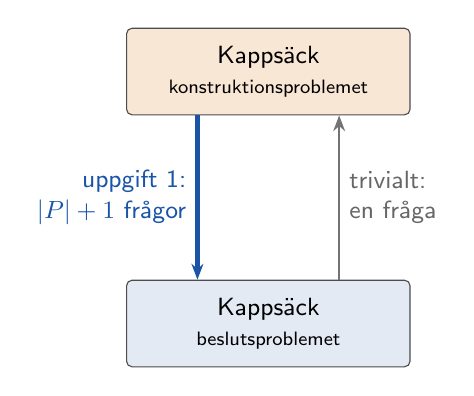
\begin{tikzpicture}
        \node[bx,fill=warnorange!18,minimum width=36mm,minimum height=11mm] (K) at (0,0) {Kappsäck\\{\scriptsize konstruktionsproblemet}};
        \node[bx,fill=kthblue!12,minimum width=36mm,minimum height=11mm] (D) at (0,-3.2) {Kappsäck\\{\scriptsize beslutsproblemet}};
        \draw[flow,line width=1.5pt,kthblue] ([xshift=-9mm]K.south) -- node[left,font=\small,align=right,text=kthblue] {uppgift 1:\\$|P|+1$ frågor} ([xshift=-9mm]D.north);
        \draw[flow,black!55] ([xshift=9mm]D.north) -- node[right,font=\small,align=left,text=black!60] {trivialt:\\en fråga} ([xshift=9mm]K.south);
      \end{tikzpicture}
    \end{column}
  \end{columns}
\end{frame}

\begin{frame}{\rabbit spelar ordningen någon roll?}{Uppgift 1}
  \centering
  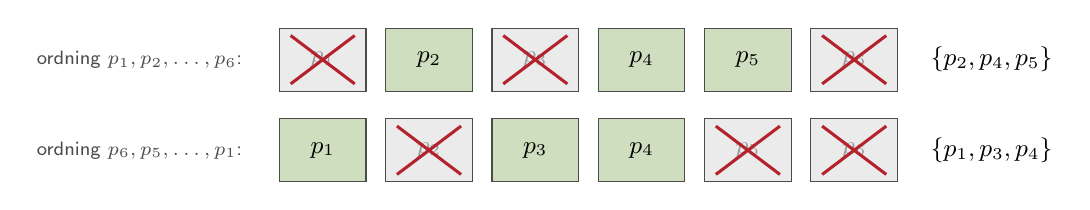
\begin{tikzpicture}
    \tikzset{pryl/.style={draw=black!70,minimum width=11mm,minimum height=8mm,font=\small,align=center,inner sep=1pt},
             bort/.style={fill=black!8,text=black!40}}
    \node[lab,anchor=east] at (-0.9,0) {ordning $p_1,p_2,\dots,p_6$:};
    \foreach \i/\st in {1/bort,2/hlok,3/bort,4/hlok,5/hlok,6/bort}
      \node[pryl,\st] (a\i) at (\i*1.35-1.35,0) {$p_\i$};
    \foreach \i in {1,3,6}
      \draw[badred,line width=1.1pt] ($(a\i.south west)+(1.5mm,1mm)$) -- ($(a\i.north east)+(-1.5mm,-1mm)$) ($(a\i.north west)+(1.5mm,-1mm)$) -- ($(a\i.south east)+(-1.5mm,1mm)$);
    \node[font=\small,anchor=west] at (7.6,0) {$\{p_2,p_4,p_5\}$};
    \begin{scope}[yshift=-1.15cm,visible on=<2->]
      \node[lab,anchor=east] at (-0.9,0) {ordning $p_6,p_5,\dots,p_1$:};
      \foreach \i/\st in {1/hlok,2/bort,3/hlok,4/hlok,5/bort,6/bort}
        \node[pryl,\st] (b\i) at (\i*1.35-1.35,0) {$p_\i$};
      \foreach \i in {2,5,6}
        \draw[badred,line width=1.1pt] ($(b\i.south west)+(1.5mm,1mm)$) -- ($(b\i.north east)+(-1.5mm,-1mm)$) ($(b\i.north west)+(1.5mm,-1mm)$) -- ($(b\i.south east)+(-1.5mm,1mm)$);
      \node[font=\small,anchor=west] at (7.6,0) {$\{p_1,p_3,p_4\}$};
    \end{scope}
  \end{tikzpicture}
  \vspace{2mm}
  \begin{itemize}
    \item<3-> För korrektheten: nej. För \emph{vilken} lösning man får: ja. Båda har vikt 10 och värde 15.
    \item<4-> Exemplet har precis två lösningar. Algoritmen returnerar den som överlever ordningen.
    \item<5-> $p_4$ ingår i alla lösningar och behålls därför alltid. $p_6$ ingår inte i någon och slängs alltid.
    \item<6-> Uppgiften ber om ''precis vilka prylar som ska packas''. Den säger inte att packningen är unik -- och det är den alltså inte.
  \end{itemize}
\end{frame}

\begin{frame}{\rabbit minimal är inte optimal}{Uppgift 1}
  \begin{columns}[T]
    \begin{column}{0.56\textwidth}
      \begin{itemize}
        \item<1-> Algoritmen lovar bara vikt $\le S$ och värde $\ge K$. Sänk målet till $K=12$ i exemplet, så returnerar den $\{p_4,p_6\}$: vikt 9, värde 13. Det bästa möjliga är 15.
        \item<2-> Vill man ha en \emph{optimal} packning: leta först upp det största $K$ som ger ja, och konstruera sedan.
        \item<3-> \textbf{Binärsökning} över $K\in[0,V]$ där $V=\sum v_i$: högst $\lceil\log_2(V+1)\rceil$ anrop. $\log V$ är högst antalet bitar i indata, så det är polynomiskt många.
        \item<4-> \textbf{Linjärsökning} $K=V,V-1,\dots$ kan kräva $V$ anrop. Det är pseudopolynomiskt: samma fälla som tabellen i verktygslådan.
      \end{itemize}
    \end{column}
    \begin{column}{0.42\textwidth}
      \centering
      \onslide<3->{%
      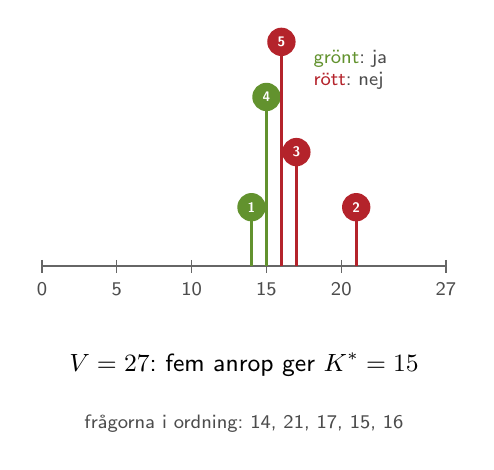
\begin{tikzpicture}[x=1.9mm]
        \draw[black!60,thick] (0,0) -- (27,0);
        \foreach \k in {0,5,10,15,20,27} {
          \draw[black!60] (\k,0.08) -- (\k,-0.08);
          \node[lab,below] at (\k,-0.08) {\k};
        }
        \foreach \k/\n/\c/\h in {14/1/okgreen/0.75,21/2/badred/0.75,17/3/badred/1.45,15/4/okgreen/2.15,16/5/badred/2.85} {
          \draw[color=\c,line width=1pt] (\k,0) -- (\k,\h);
          \node[circle,fill=\c,text=white,font=\tiny\bfseries,inner sep=1pt,minimum size=3.6mm] at (\k,\h) {\n};
        }
        \node[lab,align=left,anchor=west] at (17.5,2.5) {\textcolor{okgreen}{grönt}: ja\\\textcolor{badred}{rött}: nej};
        \node[font=\small,align=center] at (13.5,-1.25) {$V=27$: fem anrop ger $K^{*}=15$};
        \node[lab,align=center] at (13.5,-2.0) {frågorna i ordning: 14, 21, 17, 15, 16};
      \end{tikzpicture}}
    \end{column}
  \end{columns}
\end{frame}

\begin{frame}{\rabbit hur löser man kappsäck på riktigt?}{Uppgift 1}
  Dynamisk programmering, som i verktygslådan men med värden. Låt $M[i][c]$ vara det största värde som ryms i en säck med kapacitet $c$ om bara prylarna $1,\dots,i$ får användas:
  \[
    M[i][c]=\begin{cases}
      0 & \text{om } i=0\\
      M[i-1][c] & \text{om } i>0 \text{ och } c<w_i\\
      \max\bigl(M[i-1][c],\ M[i-1][c-w_i]+v_i\bigr) & \text{annars}
    \end{cases}
  \]
  \begin{columns}[T]
    \begin{column}{0.58\textwidth}
      \begin{itemize}
        \item<2-> Svaret står i $M[|P|][S]$. Själva packningen får man genom att gå baklänges i tabellen.
        \item<3-> Tid $O(|P|\cdot S)$. $|P|$ är högst indatas längd, men $S$ kan vara exponentiellt stort i antalet bitar. \textbf{Pseudopolynomiskt.}
        \item<4-> $S=10^{18}$ ryms i 60 bitar. Tabellen får $10^{18}$ kolumner.
      \end{itemize}
    \end{column}
    \begin{column}{0.4\textwidth}
      \onslide<3->{
      \begin{alertblock}{Ingen motsägelse}
        Kappsäck är NP-fullständigt \emph{och} har en pseudopolynomisk algoritm. Sådana problem kallas \emph{svagt} NP-fullständiga.
      \end{alertblock}}
      \onslide<5->{\small Algoritmen är utmärkt så länge talen är små. Det är de ofta i praktiken och sällan i bevis.}
    \end{column}
  \end{columns}
\end{frame}

\begin{frame}{\rabbit fungerar tricket för andra problem?}{Uppgift 1}
  \begin{itemize}
    \item<1-> \textbf{Hamiltoncykel:} ta bort en kant i taget. Behåll kanten om svaret blir nej. Kvar till slut: exakt en hamiltoncykel. Högst $|E|+1$ frågor, samma bevis som nyss.
    \item<2-> \textbf{\prob{Sat}:} sätt $x_1$ till sant och fråga om formeln fortfarande är satisfierbar. Om inte: sätt $x_1$ till falskt. Fortsätt med $x_2,\dots,x_n$. Högst $n+1$ frågor.
    \item<3-> \textbf{Klick, hörntäckning, delmängdssumma, \dots:} samma idé. Bygg lösningen en bit i taget och fråga efter varje steg om det går att fortsätta.
    \item<4-> \textbf{Allmänt:} för \emph{varje} NP-fullständigt problem kan lösningar konstrueras med polynomiskt många frågor till beslutsproblemet. Frågan ''går den här början att fullborda till en lösning?'' ligger nämligen själv i NP, och kan därför reduceras till problemet.
    \item<5-> Det är därför teorin kan nöja sig med ja/nej-frågor utan att något väsentligt går förlorat.
  \end{itemize}
\end{frame}

% ===================== del4-internet.tex =====================
\section{Uppgift 2: Tillförlitlighet hos Internet}

\begin{frame}{Uppgift 2: Tillförlitlighet hos Internet}{uppgiften i repris}
  \uppgiftTva
\end{frame}

% Prismat: yttre triangel 1,2,3, inre triangel 4,5,6, ekrar 1-4, 2-5, 3-6
\newcommand{\prisma}{%
  \node[vx] (v1) at (90:2.0) {1}; \node[vx] (v2) at (210:2.0) {2}; \node[vx] (v3) at (330:2.0) {3};
  \node[vx] (v4) at (90:0.8) {4}; \node[vx] (v5) at (210:0.8) {5}; \node[vx] (v6) at (330:0.8) {6};}
% Samma graf i två steg (koordinater, sedan hörn ovanpå kanterna) för figurer med overlay
\newcommand{\prismakoord}{%
  \coordinate (v1) at (90:2.0); \coordinate (v2) at (210:2.0); \coordinate (v3) at (330:2.0);
  \coordinate (v4) at (90:0.8); \coordinate (v5) at (210:0.8); \coordinate (v6) at (330:0.8);}
\newcommand{\prismanoder}[1][]{\foreach \k in {1,...,6} \node[vx,#1] at (v\k) {\k};}

% Flödesnätet i kaninhålen om certifikatet. Exemplet är G' med hörnen X, a, b, Y och
% kanterna X-a, X-b, a-b, a-Y, b-Y. \exnat ritar nätets sex noder, \exbagar{stil} dess åtta bågar.
\tikzset{
  nod/.style={vx,minimum size=7mm},
  bag/.style={-{Stealth[length=1.7mm]},black!40,line width=0.7pt},
  bagA/.style={-{Stealth[length=2.1mm]},okgreen,line width=1.6pt},
  bagB/.style={-{Stealth[length=2.1mm]},warnorange,line width=1.6pt},
  bagF/.style={-{Stealth[length=2.1mm]},kthblue,line width=1.6pt},
}
\newcommand{\exnat}{%
  \node[vx,fill=kthblue!20] (nX) at (0,0) {$X$};
  \node[nod] (ai) at (1.35,0.85) {$a_{\text{in}}$};
  \node[nod] (au) at (3.05,0.85) {$a_{\text{ut}}$};
  \node[nod] (bi) at (1.35,-0.85) {$b_{\text{in}}$};
  \node[nod] (bu) at (3.05,-0.85) {$b_{\text{ut}}$};
  \node[vx,fill=kthblue!20] (nY) at (4.4,0) {$Y$};}
\newcommand{\exbagar}[1]{%
  \draw[#1] (nX) -- (ai); \draw[#1] (nX) -- (bi);
  \draw[#1] (ai) -- (au); \draw[#1] (bi) -- (bu);
  \draw[#1] (au) -- (nY); \draw[#1] (bu) -- (nY);
  \draw[#1] (au) -- (bi); \draw[#1] (bu) -- (ai);}

\begin{frame}{Vad betyder disjunkta stigar?}{Uppgift 2}
  \begin{columns}[T]
    \begin{column}{0.6\textwidth}
      {\small\itshape ''We love internet. We hate when internet is down.''\upshape\ \ \mbox{(Lisa Li, 2019)}}
      \begin{itemize}
        \item<1-> Två stigar mellan $X$ och $Y$ är \textbf{disjunkta} om de är olika och inte har några gemensamma hörn utom ändpunkterna.
        \item<2-> Tre disjunkta stigar mellan $A$ och $B$: slå ut två datorer, vilka som helst. Varje trasig dator förstör högst en stig, så minst en finns kvar.
        \item<4-> Det gäller också åt andra hållet (Mengers sats, 1927): om två icke-grannar inte kan skiljas åt genom att $k-1$ andra hörn tas bort, så finns $k$ disjunkta stigar mellan dem.
        \item<5-> $T(X,Y)=k$ betyder alltså: förbindelsen mellan $X$ och $Y$ ska tåla $k-1$ trasiga datorer.
      \end{itemize}
    \end{column}
    \begin{column}{0.38\textwidth}
      \centering
      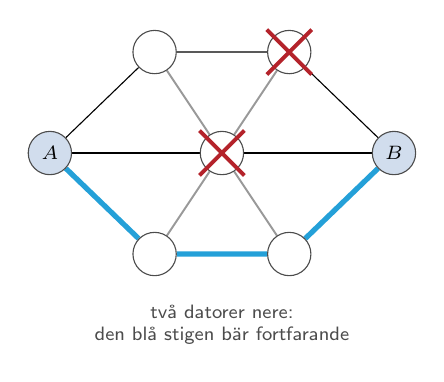
\begin{tikzpicture}[scale=0.95]
        \node[vx,fill=kthblue!20] (A) at (0,0) {$A$};
        \node[vx,fill=kthblue!20] (B) at (4.6,0) {$B$};
        \node[vx] (u1) at (1.4,1.35) {};
        \node[vx,alt=<3->{fill=badred!25}{}] (u2) at (3.2,1.35) {};
        \node[vx,alt=<3->{fill=badred!25}{}] (m) at (2.3,0) {};
        \node[vx] (d1) at (1.4,-1.35) {};
        \node[vx] (d2) at (3.2,-1.35) {};
        \begin{scope}[on background layer]
          \draw[ed] (u1) -- (m) -- (d2) (u2) -- (m) -- (d1);
          \draw[alt=<3->{ed,densely dashed}{pA}] (A) -- (u1) -- (u2) -- (B);
          \draw[alt=<3->{ed,densely dashed}{pB}] (A) -- (m) -- (B);
          \draw[pC] (A) -- (d1) -- (d2) -- (B);
        \end{scope}
        \draw[badred,line width=1.4pt,visible on=<3->] ($(u2)+(-0.3,-0.3)$) -- ($(u2)+(0.3,0.3)$) ($(u2)+(-0.3,0.3)$) -- ($(u2)+(0.3,-0.3)$);
        \draw[badred,line width=1.4pt,visible on=<3->] ($(m)+(-0.3,-0.3)$) -- ($(m)+(0.3,0.3)$) ($(m)+(-0.3,0.3)$) -- ($(m)+(0.3,-0.3)$);
        \node[lab,align=center,visible on=<3->] at (2.3,-2.3) {två datorer nere:\\den blå stigen bär fortfarande};
      \end{tikzpicture}
    \end{column}
  \end{columns}
\end{frame}

\begin{frame}{Steg 1: problemet ligger i NP}{Uppgift 2}
  \begin{columns}[T]
    \begin{column}{0.6\textwidth}
      \textbf{Indata:} $G=(V,E)$, ett tal $T(X,Y)$ för varje par av hörn, och budgeten $B$.
      \begin{itemize}
        \item<2-> \textbf{Lösning (certifikat):} en kantmängd $E'\subseteq E$ och, för varje par $(X,Y)$, en lista med $T(X,Y)$ stigar.
        \item<3-> \textbf{Verifiera:}
          \begin{enumerate}
            \item[a)] att $G'=(V,E')$ är en delgraf till $G$,
            \item[b)] att $G'$ har exakt $B$ kanter,
            \item[c)] att stigarna för varje par är rätt antal, går i $G'$ från $X$ till $Y$ och är parvis disjunkta.
          \end{enumerate}
        \item<4-> \textbf{Tid:} $O(|V|^2)$ par, och de disjunkta stigarna för ett par innehåller tillsammans högst $|V|$ hörn. Polynomiskt i indatas storlek.
      \end{itemize}
      \onslide<4->{{\small Räcker inte $E'$ ensam? Jo, men då ska verifieraren hitta stigarna själv. Det är ett \kaninhal{} längre fram.}}
    \end{column}
    \begin{column}{0.38\textwidth}
      \centering
      \onslide<2->{%
      \begin{tikzpicture}[scale=0.8]
        \prisma
        \begin{scope}[on background layer]
          \draw[ed] (v1) -- (v3) (v4) -- (v6) (v2) -- (v5);
          \draw[sel] (v1) -- (v2) -- (v3) -- (v6) -- (v5) -- (v4) -- (v1);
        \end{scope}
        \node[lab,align=center] at (0,-2.2) {$E'$: de sex blå kanterna};
      \end{tikzpicture}

      {\scriptsize
      \begin{tabular}{@{}ll@{}}
        par & stigar\\\midrule
        $(2,5)$ & 2--3--6--5,\ \ 2--1--4--5\\
        $(1,6)$ & 1--2--3--6,\ \ 1--4--5--6\\
        \dots & \dots
      \end{tabular}}}
    \end{column}
  \end{columns}
\end{frame}

\begin{frame}{Steg 2: vilket känt problem liknar det här?}{Uppgift 2}
  \begin{columns}[T]
    \begin{column}{0.6\textwidth}
      \begin{itemize}
        \item<1-> Vilket är det billigaste sättet att ge \emph{varje} par två disjunkta stigar? En ring.
        \item<2-> I en cykel finns det mellan två hörn precis två disjunkta stigar: medsols och motsols.
        \item<3-> En ring genom alla datorer, byggd av möjliga förbindelser, har ett namn. Den heter \textbf{hamiltoncykel}.
        \item<4-> \prob{Hamiltoncykel}: givet en graf $G$, finns det en cykel som passerar varje hörn exakt en gång? Känt NP-fullständigt.
        \item<5-> \textbf{Plan:} kräv två stigar för alla par, och ge precis så många kanter som en ring behöver: $T\equiv 2$ och $B=|V|$.
      \end{itemize}
    \end{column}
    \begin{column}{0.38\textwidth}
      \centering
      \onslide<2->{%
      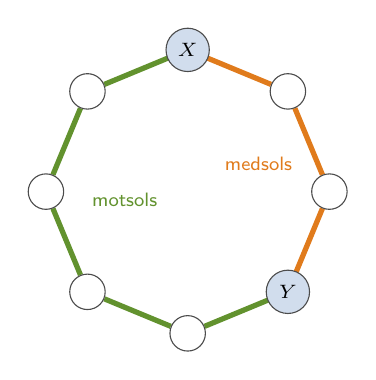
\begin{tikzpicture}
        \foreach \k in {0,...,7} \node[vx,minimum size=4.5mm] (c\k) at (\k*45+90:1.8) {};
        \node[vx,fill=kthblue!20,minimum size=5.5mm] at (c0) {$X$};
        \node[vx,fill=kthblue!20,minimum size=5.5mm] at (c5) {$Y$};
        \begin{scope}[on background layer]
          \draw[pA] (c0) -- (c1) -- (c2) -- (c3) -- (c4) -- (c5);
          \draw[pB] (c0) -- (c7) -- (c6) -- (c5);
        \end{scope}
        \node[lab,text=okgreen] at (-0.8,-0.1) {motsols};
        \node[lab,text=warnorange] at (0.9,0.35) {medsols};
      \end{tikzpicture}}
    \end{column}
  \end{columns}
\end{frame}

\begin{frame}[fragile]{Reduktionen}{Uppgift 2}
  \begin{columns}[T]
    \begin{column}{0.58\textwidth}
\begin{lstlisting}
function Hamiltoncykel(G = (V, E))
    B <- |V|
    foreach par X, Y in V do
        T(X, Y) <- 2
    return InternetBeslut(G, T, B)
\end{lstlisting}
      \begin{itemize}
        \item<2-> Ett anrop, och svaret returneras direkt: en karpreduktion.
        \item<3-> Grafen skickas vidare oförändrad. $T$ har $|V|(|V|-1)/2$ värden. Tid $O(|V|^2+|E|)$, polynomiskt i indatas storlek.
        \item<4-> Reduktionen vet inte om $G$ har en hamiltoncykel. Den behöver inte veta det. Den ska bara översätta frågan.
      \end{itemize}
    \end{column}
    \begin{column}{0.4\textwidth}
      \centering
      \begin{tikzpicture}[scale=0.72]
        \prisma
        \begin{scope}[on background layer]
          \draw[ed] (v1) -- (v2) -- (v3) -- (v1) (v4) -- (v5) -- (v6) -- (v4) (v1) -- (v4) (v2) -- (v5) (v3) -- (v6);
        \end{scope}
        \node[lab,align=center] at (0,-2.0) {$G$: 6 hörn, 9 möjliga förbindelser};
        \node[bx,fill=warnorange!18,font=\small] at (0,-3.2) {$B=6$,\quad $T(X,Y)=2$ för alla 15 par};
      \end{tikzpicture}
    \end{column}
  \end{columns}
\end{frame}

\begin{frame}{Korrekthet: $\Rightarrow$ (ja blir ja)}{Uppgift 2}
  \begin{columns}[T]
    \begin{column}{0.58\textwidth}
      \textbf{Anta} att $G$ har en hamiltoncykel $C$.
      \begin{itemize}
        \item<2-> Välj delgrafen $G'=(V,E')$ där $E'$ är precis kanterna i $C$.
        \item<3-> $G'$ har $|V|$ kanter. Budgeten $B=|V|$ håller.
        \item<4-> Ta två hörn $X$ och $Y$. De delar cykeln i två bågar, och bågarna är två disjunkta stigar mellan $X$ och $Y$. Kravet $T(X,Y)=2$ är uppfyllt.
        \item<5-> Alltså är $(G,T,B)$ en ja-instans av \prob{InternetBeslut}.
      \end{itemize}
      \onslide<5->{\vspace{1mm}{\small Det här är den lätta riktningen. Det är den nästan alltid.}}
    \end{column}
    \begin{column}{0.4\textwidth}
      \centering
      \begin{tikzpicture}[scale=0.9]
        \prisma
        \node[vx,alt=<4->{fill=kthblue!25}{}] at (v2) {2};
        \node[vx,alt=<4->{fill=kthblue!25}{}] at (v5) {5};
        \begin{scope}[on background layer]
          \draw[ed] (v1) -- (v3) (v4) -- (v6) (v2) -- (v5);
          \draw[alt=<4->{pA}{sel},visible on=<2->] (v2) -- (v3) -- (v6) -- (v5);
          \draw[alt=<4->{pB}{sel},visible on=<2->] (v2) -- (v1) -- (v4) -- (v5);
        \end{scope}
        \node[lab,align=center,visible on=<2->] at (0,-2.0) {$C$: 1--2--3--6--5--4--1};
        \node[lab,align=center,visible on=<4->] at (0,-2.45) {$X=2$, $Y=5$: \textcolor{okgreen}{2--3--6--5} och \textcolor{warnorange}{2--1--4--5}};
      \end{tikzpicture}
    \end{column}
  \end{columns}
\end{frame}

\begin{frame}{Korrekthet: $\Leftarrow$ (nej blir nej)}{Uppgift 2}
  \begin{columns}[T]
    \begin{column}{0.6\textwidth}
      \textbf{Anta} att det finns en delgraf $G'$ med $|V|$ kanter där alla par har två disjunkta stigar.
      \begin{enumerate}
        \item<2-> Varje hörn har grad minst 2 i $G'$: två disjunkta stigar från $X$ måste lämna $X$ längs olika kanter.
        \item<3-> Gradsumman är $2|E'|=2|V|$. Alla grader är alltså \emph{exakt} 2.
        \item<4-> $G'$ är sammanhängande, för det finns stigar mellan alla par.
        \item<5-> En sammanhängande graf där alla hörn har grad 2 är en enda cykel genom alla hörn. $G'$ är en hamiltoncykel i $G$. \hfill$\Box$
      \end{enumerate}
      \onslide<6->{\vspace{1mm}{\small Anton Grensjös bilder (2017) frågar: unionen av två disjunkta stigar är en cykel, men varför går den genom \emph{alla} hörn? Svaret är gradräkningen i steg 2.}}
    \end{column}
    \begin{column}{0.38\textwidth}
      \centering
      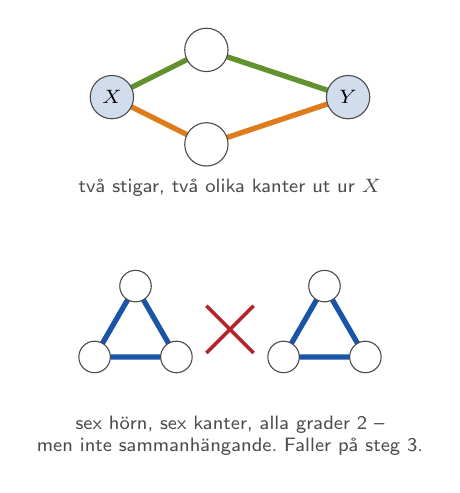
\begin{tikzpicture}
        \coordinate (X) at (0,0); \coordinate (a) at (1.2,0.6); \coordinate (b) at (1.2,-0.6); \coordinate (Y) at (3.0,0);
        \draw[pA,visible on=<2->] (X) -- (a) -- (Y);
        \draw[pB,visible on=<2->] (X) -- (b) -- (Y);
        \node[vx,fill=kthblue!20,visible on=<2->] at (X) {$X$};
        \node[vx,visible on=<2->] at (a) {};
        \node[vx,visible on=<2->] at (b) {};
        \node[vx,fill=kthblue!20,visible on=<2->] at (Y) {$Y$};
        \node[lab,visible on=<2->] at (1.5,-1.15) {två stigar, två olika kanter ut ur $X$};
        \begin{scope}[yshift=-3.0cm,xshift=0.3cm]
          \foreach \k in {0,1,2} {
            \coordinate (s\k) at (\k*120+90:0.6);
            \coordinate (t\k) at ($(2.4,0)+(\k*120+90:0.6)$);}
          \draw[sel,visible on=<5->] (s0) -- (s1) -- (s2) -- cycle (t0) -- (t1) -- (t2) -- cycle;
          \foreach \k in {0,1,2} {
            \node[vx,minimum size=4mm,visible on=<5->] at (s\k) {};
            \node[vx,minimum size=4mm,visible on=<5->] at (t\k) {};}
          \node[lab,align=center,visible on=<5->] at (1.2,-1.3) {sex hörn, sex kanter, alla grader 2 --\\men inte sammanhängande. Faller på steg 3.};
          \draw[badred,line width=1.3pt,visible on=<5->] (0.9,-0.25) -- (1.5,0.35) (0.9,0.35) -- (1.5,-0.25);
        \end{scope}
      \end{tikzpicture}
    \end{column}
  \end{columns}
\end{frame}

\begin{frame}{Exempel: det är budgeten som gör jobbet}{Uppgift 2}
  \begin{columns}[T]
    \begin{column}{0.58\textwidth}
      \begin{itemize}
        \item<1-> $K_{2,3}$: fem hörn, sex kanter.
        \item<2-> Med alla sex kanterna har varje par två disjunkta stigar. Nätet tål en trasig dator var som helst.
        \item<3-> Reduktionen sätter $B=|V|=5$. En kant måste alltså bort -- och då får ett hörn grad 1.
        \item<4-> Svaret blir nej, och det ska det bli: $K_{2,3}$ har ingen hamiltoncykel. (Den är bipartit med ett udda antal hörn.)
        \item<5-> Hade reduktionen satt $B=6$ hade svaret blivit ja -- och fel. Budgeten ska vara precis $|V|$.
      \end{itemize}
    \end{column}
    \begin{column}{0.4\textwidth}
      \centering
      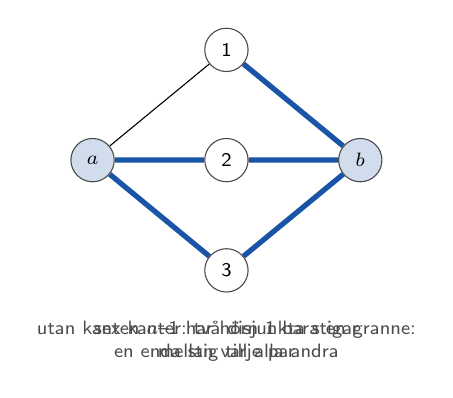
\begin{tikzpicture}
        \node[vx,fill=kthblue!20] (a) at (-1.7,0) {$a$};
        \node[vx,fill=kthblue!20] (b) at (1.7,0) {$b$};
        \node[vx,alt=<3->{fill=badred!25}{}] (m1) at (0,1.4) {1};
        \node[vx] (m2) at (0,0) {2};
        \node[vx] (m3) at (0,-1.4) {3};
        \begin{scope}[on background layer]
          \draw[sel] (a) -- (m2) -- (b) (a) -- (m3) -- (b) (m1) -- (b);
          \draw[alt=<3->{badred,densely dashed,line width=1.2pt}{sel}] (a) -- (m1);
        \end{scope}
        \node[lab,align=center,visible on=<3->] at (0,-2.3) {utan kanten $a$--1 har hörn 1 bara en granne:\\en enda stig till alla andra};
        \node[lab,align=center,visible on=<2| handout:0>] at (0,-2.3) {sex kanter: två disjunkta stigar\\mellan varje par};
      \end{tikzpicture}
    \end{column}
  \end{columns}
\end{frame}

% ---------------------------------------------------------------- kaninhål: budgeten
\begin{frame}{\rabbit hur noga är det med budgeten?}{Uppgift 2}
  \begin{columns}[T]
    \begin{column}{0.62\textwidth}
      \begin{itemize}
        \item<1-> \textbf{Talet $B$ är hela reduktionen.} Med $B<|V|$ räcker kanterna inte till grad 2 överallt: alltid nej. Med $B>|V|$ godkänns grafer utan hamiltoncykel.
        \item<2-> Med $B=|V|+1$ godkänns 20 av de 1\,024 graferna med fem numrerade hörn fast de saknar hamiltoncykel. Det minsta motexemplet är $K_{2,3}$.
        \item<3-> \textbf{Det som inte spelar roll} är om ''bestående av $B$ kanter'' läses som exakt $B$ (Anton Grensjö, Lisa Li) eller högst $B$ (Alice Heavey).
        \item<4-> Fler kanter förstör aldrig en stig. En lösning med färre kanter kan fyllas på till exakt $B$ så länge $B\le|E|$: samma ja-instanser.
        \item<5-> Beviset för $\Leftarrow$ behöver bara ''högst $|V|$ kanter''. Att de är minst $|V|$ ger gradräkningen själv.
      \end{itemize}
    \end{column}
    \begin{column}{0.36\textwidth}
      \centering
      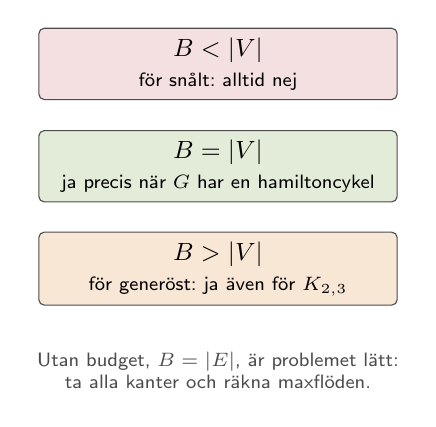
\begin{tikzpicture}
        \node[bx,fill=badred!14,text width=42mm] at (0,1.55) {$B<|V|$\\{\scriptsize för snålt: alltid nej}};
        \node[bx,fill=okgreen!18,text width=42mm] at (0,0.25) {$B=|V|$\\{\scriptsize ja precis när $G$ har en hamiltoncykel}};
        \node[bx,fill=warnorange!18,text width=42mm] at (0,-1.05) {$B>|V|$\\{\scriptsize för generöst: ja även för $K_{2,3}$}};
        \node[lab,align=flush center,text width=46mm] at (0,-2.35) {Utan budget, $B=|E|$, är problemet lätt:\\ta alla kanter och räkna maxflöden.};
      \end{tikzpicture}
    \end{column}
  \end{columns}
\end{frame}

% ---------------------------------------------------------------- kaninhål: hamiltonstig
\begin{frame}{\rabbit går det med hamiltonstig i stället?}{Uppgift 2}
  \begin{columns}[T]
    \begin{column}{0.62\textwidth}
      \begin{itemize}
        \item<1-> \prob{Hamiltonstig}: finns en stig som passerar varje hörn exakt en gång? Också känt NP-fullständigt, så försöket är rimligt.
        \item<2-> \textbf{Frestande:} en stig har $|V|-1$ kanter och håller ihop alla hörn. Skicka $G$ vidare oförändrad med $T\equiv1$ och $B=|V|-1$.
        \item<3-> \textbf{Fel.} Varje spännande träd godkänns. Stjärnan ger ja men saknar hamiltonstig. Fel svar för 4 av 64 grafer med fyra hörn och 95 av 1\,024 med fem.
        \item<4-> Varningsklockan: med $T\equiv1$ är problemet lätt. En korrekt reduktion dit vore ett bevis för $\mathrm{P}=\mathrm{NP}$.
        \item<5-> Andra tal hjälper inte. En stig klarar aldrig ett krav $T(X,Y)\ge2$, och allt en stig klarar, klarar varje spännande träd med lika många kanter. Stigen måste bli en ring.
      \end{itemize}
    \end{column}
    \begin{column}{0.36\textwidth}
      \centering
      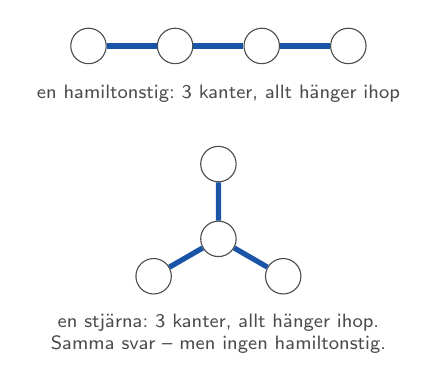
\begin{tikzpicture}
        \foreach \k in {0,1,2,3} \node[vx,minimum size=4.5mm,visible on=<2->] (p\k) at (\k*1.1,0) {};
        \draw[sel,visible on=<2->] (p0) -- (p1) -- (p2) -- (p3);
        \node[lab,align=center,visible on=<2->] at (1.65,-0.6) {en hamiltonstig: 3 kanter, allt hänger ihop};
        \begin{scope}[shift={(1.65,-2.45)}]
          \node[vx,minimum size=4.5mm,visible on=<3->] (c) at (0,0) {};
          \foreach \a/\n in {90/l1,210/l2,330/l3} \node[vx,minimum size=4.5mm,visible on=<3->] (\n) at (\a:0.95) {};
          \draw[sel,visible on=<3->] (c) -- (l1) (c) -- (l2) (c) -- (l3);
          \node[lab,align=center,visible on=<3->] at (0,-1.2) {en stjärna: 3 kanter, allt hänger ihop.\\Samma svar -- men ingen hamiltonstig.};
        \end{scope}
      \end{tikzpicture}
    \end{column}
  \end{columns}
\end{frame}

\begin{frame}[fragile]{\rabbit hamiltonstig med ett extra hörn}{Uppgift 2}
  \begin{columns}[T]
    \begin{column}{0.6\textwidth}
\begin{lstlisting}
function Hamiltonstig(G = (V, E))
    H <- G + nytt hörn z, granne med alla i V
    B <- |V| + 1
    foreach par X, Y in H do
        T(X, Y) <- 2
    return InternetBeslut(H, T, B)
\end{lstlisting}
      \begin{itemize}
        \item<2-> $\Rightarrow$: en hamiltonstig $v_1,\dots,v_n$ i $G$ sluts till ringen $z,v_1,\dots,v_n,z$ i $H$. Den har $|V|+1$ kanter.
        \item<3-> $\Leftarrow$: beviset från förut ger en hamiltoncykel i $H$. Ta bort $z$ ur den: kvar blir en hamiltonstig i $G$.
        \item<4-> Budgeten är antalet hörn i $H$, alltså $|V|+1$. Med en kant till går det fel: stjärnan plus $z$ innehåller $K_{2,3}$.
        \item<5-> Givna ändpunkter $s$ och $t$? Ge $z$ bara kanterna till $s$ och $t$.
      \end{itemize}
    \end{column}
    \begin{column}{0.38\textwidth}
      \centering
      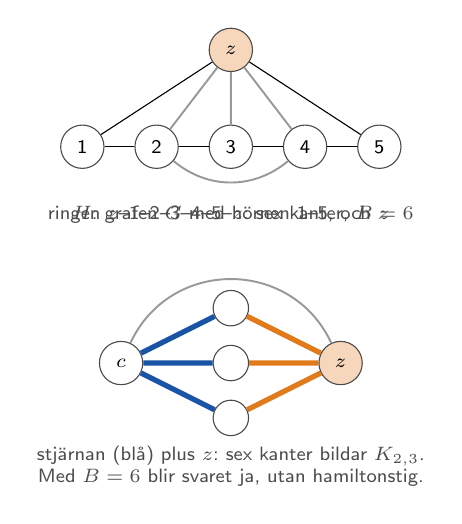
\begin{tikzpicture}[scale=0.82]
        \foreach \k in {1,...,5} \node[vx] (g\k) at (\k*1.15-1.15,0) {\k};
        \node[vx,fill=warnorange!30] (z) at (2.3,1.5) {$z$};
        \draw[ed] (g2) to[bend right=40] (g4);
        \draw[ed] (z) -- (g2) (z) -- (g3) (z) -- (g4);
        \draw[alt=<2->{sel}{ed}] (g1) -- (g2) -- (g3) -- (g4) -- (g5);
        \draw[alt=<2->{sel}{ed}] (z) -- (g1) (z) -- (g5);
        \node[lab,align=center,visible on=<1| handout:0>] at (2.3,-1.05) {$H$: grafen $G$ med hörnen 1--5, och $z$};
        \node[lab,align=center,visible on=<2->] at (2.3,-1.05) {ringen $z$--1--2--3--4--5--$z$: sex kanter, $B=6$};
        \begin{scope}[shift={(2.3,-3.35)}]
          \node[vx,visible on=<4->] (c) at (-1.7,0) {$c$};
          \node[vx,fill=warnorange!30,visible on=<4->] (zz) at (1.7,0) {$z$};
          \foreach \y/\n in {0.85/s1,0/s2,-0.85/s3} \node[vx,minimum size=4.5mm,visible on=<4->] (\n) at (0,\y) {};
          \draw[ed,visible on=<4->] (c) to[out=65,in=115,looseness=1.2] (zz);
          \draw[sel,visible on=<4->] (c) -- (s1) (c) -- (s2) (c) -- (s3);
          \draw[pB,visible on=<4->] (zz) -- (s1) (zz) -- (s2) (zz) -- (s3);
          \node[lab,align=center,visible on=<4->] at (0,-1.6) {stjärnan (blå) plus $z$: sex kanter bildar $K_{2,3}$.\\Med $B=6$ blir svaret ja, utan hamiltonstig.};
        \end{scope}
      \end{tikzpicture}
    \end{column}
  \end{columns}
\end{frame}

% ---------------------------------------------------------------- kaninhål: certifikatet och flödet
\begin{frame}{\rabbit räcker kanterna som certifikat?}{Uppgift 2}
  \begin{columns}[T]
    \begin{column}{0.6\textwidth}
      \begin{itemize}
        \item<1-> Steg 1 lade stigarna i certifikatet, som Anton Grensjö (2017). Det säkra valet: verifieraren kontrollerar, den letar aldrig.
        \item<2-> Lisa Li (2019) låter lösningen vara enbart $G'$. Då ska verifieraren själv avgöra om stigarna finns.
        \item<3-> \textbf{Invändning:} Ford--Fulkerson räknar ut ett flöde, inga stigar. Och stigarna algoritmen går längs under arbetet behöver inte vara disjunkta.
        \item<4-> Båda påståendena är sanna. Ändå räcker kanterna:
      \end{itemize}
      \begin{block}<4->{Sats}
        Givet $G'$, $X$ och $Y$ kan man på polynomisk tid räkna ut det största antalet disjunkta stigar mellan $X$ och $Y$ -- och stigarna själva.
      \end{block}
    \end{column}
    \begin{column}{0.38\textwidth}
      \centering
      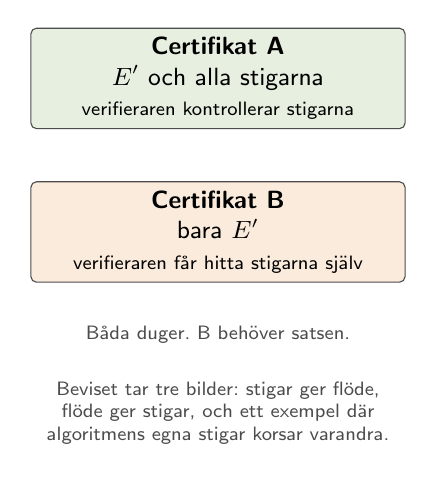
\begin{tikzpicture}
        \node[bx,fill=okgreen!15,text width=44mm] at (0,1.5) {\textbf{Certifikat A}\\$E'$ och alla stigarna\\{\scriptsize verifieraren kontrollerar stigarna}};
        \node[bx,fill=warnorange!15,text width=44mm,visible on=<2->] at (0,-0.45) {\textbf{Certifikat B}\\bara $E'$\\{\scriptsize verifieraren får hitta stigarna själv}};
        \node[lab,align=center,visible on=<4->] at (0,-1.75) {Båda duger. B behöver satsen.};
        \node[lab,align=flush center,text width=46mm,visible on=<5->] at (0,-2.75) {Beviset tar tre bilder: stigar ger flöde,\\flöde ger stigar, och ett exempel där\\algoritmens egna stigar korsar varandra.};
      \end{tikzpicture}
    \end{column}
  \end{columns}
\end{frame}

\begin{frame}{\rabbit från stigar till flöde}{Uppgift 2}
  \begin{columns}[T]
    \begin{column}{0.6\textwidth}
      \textbf{Bygg ett flödesnät} $N$ av $G'$ för paret $(X,Y)$:
      \begin{enumerate}
        \item $X$ blir källa och $Y$ utlopp. De delas inte: $X$ får bara bågar ut, $Y$ bara bågar in.
        \item Varje annat hörn $v$ blir två noder med en båge $v_{\text{in}}\to v_{\text{ut}}$.
        \item Varje kant $\{u,v\}$ blir två bågar: $u_{\text{ut}}\to v_{\text{in}}$ och $v_{\text{ut}}\to u_{\text{in}}$.
        \item Alla bågar får kapacitet 1.
      \end{enumerate}
      \begin{itemize}
        \item<2-> \textbf{Lätta hållet:} $k$ disjunkta stigar i $G'$ ger ett flöde av storlek $k$ i $N$. Skicka en enhet längs varje stig. Stigarna delar varken hörn eller kanter, så ingen kapacitet överskrids.
        \item<3-> Maxflödet är alltså \emph{minst} antalet disjunkta stigar. Kan det vara större?
      \end{itemize}
    \end{column}
    \begin{column}{0.38\textwidth}
      \centering
      \begin{tikzpicture}[scale=0.9]
        \node[vx,fill=kthblue!20] (gX) at (0.5,0) {$X$};
        \node[vx] (ga) at (2.2,0.65) {$a$};
        \node[vx] (gb) at (2.2,-0.65) {$b$};
        \node[vx,fill=kthblue!20] (gY) at (3.9,0) {$Y$};
        \draw[ed] (ga) -- (gb);
        \draw[alt=<2->{pA}{ed}] (gX) -- (ga) -- (gY);
        \draw[alt=<2->{pB}{ed}] (gX) -- (gb) -- (gY);
        \node[lab] at (2.2,-1.25) {$G'$: fyra hörn, fem kanter};
        \draw[flow] (2.2,-1.5) -- (2.2,-1.95);
        \begin{scope}[shift={(0,-3.2)}]
          \exnat
          \exbagar{bag}
          \draw[bagA,visible on=<2->] (nX) -- (ai); \draw[bagA,visible on=<2->] (ai) -- (au); \draw[bagA,visible on=<2->] (au) -- (nY);
          \draw[bagB,visible on=<2->] (nX) -- (bi); \draw[bagB,visible on=<2->] (bi) -- (bu); \draw[bagB,visible on=<2->] (bu) -- (nY);
          \node[lab,align=center] at (2.2,-1.6) {$N$: sex noder, åtta bågar.\\Nod och båge = hörn och riktad kant i nätet.};
        \end{scope}
      \end{tikzpicture}
    \end{column}
  \end{columns}
\end{frame}

\begin{frame}{\rabbit från flöde till stigar}{Uppgift 2}
  \begin{columns}[T]
    \begin{column}{0.66\textwidth}
      \small
      Ford--Fulkerson ger ett maxflöde $f$ i $N$. Säg att det har värdet $k$.
      \begin{enumerate}
        \item<1-> \textbf{Heltal.} Flödet börjar på 0 och varje utökning ändrar det med ett heltal. Alltså: 0 eller 1 på varje båge.
        \item<2-> \textbf{En enhet per nod.} Bågen $v_{\text{in}}\to v_{\text{ut}}$ rymmer 1. Den är enda vägen ut ur $v_{\text{in}}$ och enda vägen in i $v_{\text{ut}}$. Varje nod utom $X$ och $Y$ har därför högst en flödesbåge in, och lika många ut.
        \item<3-> \textbf{Följ flödet.} Börja i $X$ och gå längs flödesbågar. Varje nod på vägen har precis en flödesbåge ut. Ingen nod nås två gånger, för den hade då haft två flödesbågar in. Nätet är ändligt, så vandringen tar slut -- och det kan den bara göra i $Y$.
        \item<4-> \textbf{$k$ stigar.} Ur $X$ går $k$ flödesbågar. De ger $k$ vandringar, som av samma skäl aldrig möts före $Y$. Slå ihop $v_{\text{in}}$ och $v_{\text{ut}}$ igen: $k$ disjunkta stigar i $G'$. \hfill$\Box$
      \end{enumerate}
      \onslide<5->{Med det lätta hållet från förra bilden: maxflödet är precis det största antalet disjunkta stigar, och stigarna står att läsa i flödet. Flödesbågar som blir över bildar slutna cykler och kastas.}
    \end{column}
    \begin{column}{0.32\textwidth}
      \centering
      \onslide<2->{%
      \begin{tikzpicture}
        \node[vx] (v) at (0,0) {$v$};
        \foreach \a in {150,210,30,-30} \draw[ed] (v) -- (\a:1.1);
        \node[lab] at (0,-0.75) {ett hörn i $G'$};
        \draw[flow] (0,-1.05) -- (0,-1.55);
        \node[nod] (vi) at (-0.9,-2.5) {$v_{\text{in}}$};
        \node[nod] (vo) at (0.9,-2.5) {$v_{\text{ut}}$};
        \draw[bag] ($(vi)+(150:1.1)$) -- (vi);
        \draw[bagF] ($(vi)+(210:1.1)$) -- (vi);
        \draw[bagF] (vi) -- node[above,font=\scriptsize,text=kthblue] {kap.\ 1} (vo);
        \draw[bagF] (vo) -- ($(vo)+(30:1.1)$);
        \draw[bag] (vo) -- ($(vo)+(-30:1.1)$);
        \node[lab,align=center] at (0,-3.6) {blått: bågar med flöde 1.\\Högst en in, och då precis en ut.};
      \end{tikzpicture}}
    \end{column}
  \end{columns}
\end{frame}

\begin{frame}{\rabbit algoritmens stigar är inte svaret}{Uppgift 2}
  \begin{columns}[T]
    \begin{column}{0.32\textwidth}
      \centering
      \begin{tikzpicture}[scale=0.8]
        \exnat
        \exbagar{bag}
        \draw[bagA] (nX) -- (ai); \draw[bagA] (ai) -- (au); \draw[bagA] (au) -- (bi); \draw[bagA] (bi) -- (bu); \draw[bagA] (bu) -- (nY);
        \node[lab,align=center] at (2.2,-1.75) {första utökande stigen:\\$X\to a\to b\to Y$};
      \end{tikzpicture}
    \end{column}
    \begin{column}{0.32\textwidth}
      \centering
      \onslide<2->{%
      \begin{tikzpicture}[scale=0.8]
        \exnat
        \exbagar{bag}
        \draw[bagA,okgreen!55,line width=1.0pt] (nX) -- (ai); \draw[bagA,okgreen!55,line width=1.0pt] (ai) -- (au);
        \draw[bagA,okgreen!55,line width=1.0pt] (au) -- (bi); \draw[bagA,okgreen!55,line width=1.0pt] (bi) -- (bu);
        \draw[bagA,okgreen!55,line width=1.0pt] (bu) -- (nY);
        \draw[bagB] (nX) -- (bi); \draw[bagB] (au) -- (nY);
        \draw[bagB,densely dashed] (bi) to[bend left=28] (au);
        \node[lab,align=center] at (2.2,-1.75) {andra utökande stigen:\\$X\to b$, bakåt till $a$, $a\to Y$};
      \end{tikzpicture}}
    \end{column}
    \begin{column}{0.32\textwidth}
      \centering
      \onslide<3->{%
      \begin{tikzpicture}[scale=0.8]
        \exnat
        \exbagar{bag}
        \draw[bagF] (nX) -- (ai); \draw[bagF] (ai) -- (au); \draw[bagF] (au) -- (nY);
        \draw[bagF] (nX) -- (bi); \draw[bagF] (bi) -- (bu); \draw[bagF] (bu) -- (nY);
        \node[lab,align=center] at (2.2,-1.75) {det färdiga flödet:\\$X\to a\to Y$ och $X\to b\to Y$};
      \end{tikzpicture}}
    \end{column}
  \end{columns}
  \vspace{1mm}
  \begin{itemize}
    \item<1-> Ford--Fulkerson med djupetförstsökning på nätet $N$ från exemplet. Första sökningen råkar gå $X\to a\to b\to Y$.
    \item<2-> Andra sökningen går $X\to b$, sedan \emph{bakåt} över bågen $a_{\text{ut}}\to b_{\text{in}}$ och ut via $a\to Y$. Algoritmens två stigar går båda genom $a$ och $b$. Invändningen stämmer.
    \item<3-> Men bakåtsteget tog bort flödet mellan $a$ och $b$. Kvar står två disjunkta stigar.
    \item<4-> Stigarna läses av ur det \textbf{färdiga flödet}, inte ur algoritmens historia. Det är samma sak som i labb 3: de utökande stigarna backar över matchade kanter, men matchningen läses av ur flödet.
  \end{itemize}
\end{frame}

\begin{frame}{\rabbit vad betyder det för NP-beviset?}{Uppgift 2}
  \begin{columns}[T]
    \begin{column}{0.62\textwidth}
      \begin{itemize}
        \item<1-> \textbf{Verifierare med bara kanterna:} bygg $N$ för varje par, räkna maxflödet och jämför med $T(X,Y)$. Stigarna behöver aldrig skrivas ut.
        \item<2-> \textbf{Tid:} högst $|V|^2$ par. Maxflödet är högst $|V|-1$, så det blir högst $|V|$ sökningar à $O(|V|+|E|)$ per par. Polynomiskt.
        \item<3-> \textbf{Båda certifikaten duger.} Med stigarna i certifikatet behövs ingen flödesteori. Med bara kanterna vilar beviset på satsen.
        \item<4-> På en tenta: välj det certifikat vars verifiering du kan bevisa. Certifikatet får innehålla hur mycket hjälp som helst, bara det är polynomiskt långt.
        \item<5-> Med satsen om maxflöde och minsta snitt följer dessutom Mengers sats från början av avsnittet.
      \end{itemize}
    \end{column}
    \begin{column}{0.36\textwidth}
      \centering
      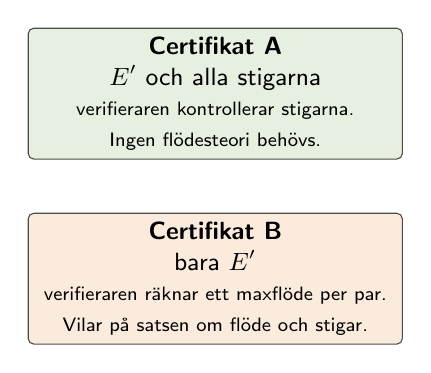
\begin{tikzpicture}
        \node[bx,fill=okgreen!15,text width=44mm] at (0,1.6) {\textbf{Certifikat A}\\$E'$ och alla stigarna\\{\scriptsize verifieraren kontrollerar stigarna.}\\{\scriptsize Ingen flödesteori behövs.}};
        \node[bx,fill=warnorange!15,text width=44mm] at (0,-0.75) {\textbf{Certifikat B}\\bara $E'$\\{\scriptsize verifieraren räknar ett maxflöde per par.}\\{\scriptsize Vilar på satsen om flöde och stigar.}};
      \end{tikzpicture}
    \end{column}
  \end{columns}
\end{frame}

% ---------------------------------------------------------------- kaninhål: det finstilta
\begin{frame}{\rabbit det finstilta}{Uppgift 2}
  \begin{itemize}
    \item<1-> \textbf{Hörndisjunkta eller kantdisjunkta stigar?} Uppgiften säger ''helt disjunkta (utom ändpunkterna)'', alltså hörndisjunkta. Reduktionen fungerar ordagrant också för kantdisjunkta stigar: gradargumentet är detsamma. Flödesbeviset likaså, utan hörndelning: stryk flöde som går åt båda hållen på samma kant, dra ut en vandring i taget och korta av slingorna.
    \item<2-> \textbf{Riktigt små grafer.} En graf med ett eller två hörn har ingen hamiltoncykel, och ett ensamt hörn är en hamiltonstig som inte kan slutas till en ring. En karpreduktion måste ge rätt svar för \emph{alla} instanser, så ett pedantiskt bevis tar de minsta graferna för sig och returnerar en fix instans.
    \item<3-> \textbf{Jättestora $T(X,Y)$.} Ett par kan ha högst $|V|-1$ disjunkta stigar, en per granne. Kräver indata $T(X,Y)=10^{100}$ är svaret nej, och nej-instanser behöver inga certifikat. Certifikatet med stigar är alltså polynomiskt långt.
    \item<4-> \textbf{Kontrollräknat.} Ett program har prövat cykelreduktionen på samtliga 33\,864 grafer med tre till sex numrerade hörn, stigreduktionen på samtliga 33\,866 med två till sex, och flödessatsen mot uttömmande sökning på 8\,660 par i slumpgrafer. Rätt varje gång. Det är inget bevis, men det är betryggande.
  \end{itemize}
\end{frame}

\begin{frame}{\rabbit ett är lätt, två är svårt}{Uppgift 2}
  \begin{columns}[T]
    \begin{column}{0.6\textwidth}
      \begin{itemize}
        \item<1-> $T\equiv 1$: varje par ska bara hänga ihop. Ett spännande träd räcker, så svaret är ja precis när $G$ är sammanhängande och $|V|-1\le B\le|E|$. Linjär tid med BFS.
        \item<2-> $T\equiv 2$: NP-fullständigt. Det har vi just visat.
        \item<3-> Från träd till cykel, från lätt till svårt. Samma språng kommer tillbaka i uppgift 4: två tidsenheter är lätt, tre är svårt.
        \item<4-> I litteraturen heter problemet \emph{survivable network design}. Varianten med hörndisjunkta stigar kallas VC-SNDP, den med kantdisjunkta EC-SNDP.
        \item<5-> För EC-SNDP finns en algoritm som alltid hamnar inom en faktor 2 från det billigaste nätet (Jain, 2001). Sådana approximationsalgoritmer är ämnet för nästa övning.
      \end{itemize}
    \end{column}
    \begin{column}{0.38\textwidth}
      \centering
      \begin{tikzpicture}[scale=0.7]
        \begin{scope}
          \prismakoord
          \draw[ed] (v1) -- (v3) (v4) -- (v5) -- (v6) -- (v4);
          \draw[sel] (v1) -- (v2) -- (v3) (v1) -- (v4) (v2) -- (v5) (v3) -- (v6);
          \prismanoder[minimum size=4.5mm]
          \node[lab,align=center] at (0,-1.75) {$T\equiv1$: ett spännande träd, 5 kanter};
        \end{scope}
        \begin{scope}[shift={(0,-5.1)}]
          \prismakoord
          \draw[ed,visible on=<2->] (v1) -- (v3) (v4) -- (v6) (v2) -- (v5);
          \draw[sel,visible on=<2->] (v1) -- (v2) -- (v3) -- (v6) -- (v5) -- (v4) -- (v1);
          \prismanoder[minimum size=4.5mm,visible on=<2->]
          \node[lab,align=center,visible on=<2->] at (0,-1.75) {$T\equiv2$: en hamiltoncykel, 6 kanter};
        \end{scope}
      \end{tikzpicture}
    \end{column}
  \end{columns}
\end{frame}

% ===================== del5-hastad.tex =====================
\section{Uppgift 3: Håstads leksaksaffär}

\begin{frame}{Uppgift 3: Håstads leksaksaffär}{uppgiften i repris}
  \uppgiftTre
\end{frame}

\begin{frame}{Pusslet finns på riktigt}{Uppgift 3}
  \centering
  \foto{height=3.3cm}{hastad-kort.jpg}\hspace{3mm}\foto{height=3.3cm}{hastad-lada.jpg}\\[0.5mm]
  {\scriptsize\textcolor{softgray}{Foto ur Anton Grensjös övningsbilder (2017). Till höger: lådan med sina lister och ett kort på plats.}}
  \vspace{1mm}
  \begin{columns}[T]
    \begin{column}{0.48\textwidth}
      \begin{itemize}
        \item<1-> Fyra kort med tre rader och två kolumner. Det fjärde har hål i bara den ena kolumnen. Lägg det på minnet.
        \item<2-> Listerna i lådan passar i urgröpningarna. Ett kort går därför bara att lägga på två sätt.
      \end{itemize}
    \end{column}
    \begin{column}{0.48\textwidth}
      \begin{itemize}
        \item<3-> \textbf{Att vända ett kort är att spegla det:} vänster och höger kolumn byter plats. Raderna ligger kvar.
        \item<4-> Det är allt pusslet handlar om: ett binärt val per kort.
      \end{itemize}
    \end{column}
  \end{columns}
\end{frame}

\begin{frame}{Formalisering: vad är ett kort, och vad är en lösning?}{Uppgift 3}
  \begin{columns}[T]
    \begin{column}{0.58\textwidth}
      \begin{itemize}
        \item<1-> Ett kort med $m$ rader beskrivs av två bitvektorer med $m$ bitar var: \textbf{vänsterkolumnen} och \textbf{högerkolumnen}. 1 betyder igenfyllt, 0 betyder hål.
        \item<2-> Ett vänt kort är samma kort med kolumnerna ombytta.
        \item<3-> En \textbf{lösning} är ett val per kort: rättvänt eller vänt. Med $n$ kort finns $2^n$ sätt att lägga dem.
        \item<4-> En position (rad $j$, kolumn vänster eller höger) är \textbf{täckt} om minst ett av korten, så som det ligger, är igenfyllt där.
        \item<5-> Pusslet är löst när alla $2m$ positioner är täckta. Ordningen i högen spelar ingen roll.
      \end{itemize}
    \end{column}
    \begin{column}{0.4\textwidth}
      \centering
      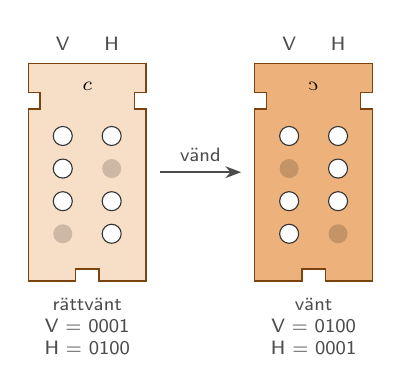
\begin{tikzpicture}[scale=1.15]
        \hkort{0}{0}{0,0,0,1}{0,1,0,0}{$c$}{kort}
        \node[lab] at (0.38,2.62) {V};
        \node[lab] at (0.92,2.62) {H};
        \begin{scope}[visible on=<2->]
          \hkort{2.5}{0}{0,1,0,0}{0,0,0,1}{\spegel{$c$}}{kortvand}
          \node[lab] at (2.88,2.62) {V};
          \node[lab] at (3.42,2.62) {H};
          \draw[flow] (1.45,1.2) -- node[above,lab] {vänd} (2.35,1.2);
        \end{scope}
        \node[lab,align=center] at (0.65,-0.5) {rättvänt\\V = 0001\\H = 0100};
        \node[lab,align=center,visible on=<2->] at (3.15,-0.5) {vänt\\V = 0100\\H = 0001};
      \end{tikzpicture}
    \end{column}
  \end{columns}
\end{frame}

\begin{frame}{Steg 1: \prob{Toys} ligger i NP}{Uppgift 3}
  \begin{columns}[T]
    \begin{column}{0.6\textwidth}
      \begin{itemize}
        \item<1-> \textbf{Lösning (certifikat):} en beskrivning av hur korten ska läggas, alltså en bit per kort.
        \item<2-> \textbf{Verifiera:} lägg korten i lådan enligt beskrivningen och titta efter om man ser botten.
        \item<3-> Facit: det räcker med en blick. För en dator är blicken en dubbelslinga: för var och en av de $2m$ positionerna, finns det ett kort som är igenfyllt där?
        \item<4-> \textbf{Tid:} $O(n\cdot m)$, linjärt i indatas storlek. Indata är $n$ kort med $2m$ bitar var.
        \item<5-> Certifikatet är $n$ bitar långt. Här finns inga tal att bli lurad av, så pseudopolynomiska fällor saknas helt.
      \end{itemize}
    \end{column}
    \begin{column}{0.38\textwidth}
      \centering
      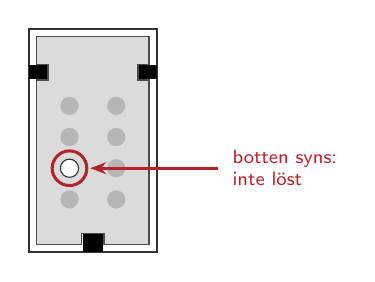
\begin{tikzpicture}[scale=1.1]
        \draw[black!80,line width=0.8pt] (-0.09,-0.09) rectangle (1.39,2.49);
        \hkort{0}{0}{1,1,0,1}{1,1,1,1}{}{korthog}
        \fill[black] (-0.09,1.905) rectangle (0.12,2.075);
        \fill[black] (1.18,1.905) rectangle (1.39,2.075);
        \fill[black] (0.535,-0.09) rectangle (0.765,0.12);
        \draw[badred,line width=1.1pt] (0.38,0.88) circle (0.2);
        \draw[badred,-{Stealth[length=2mm]},line width=1pt] (2.1,0.88) -- (0.62,0.88);
        \node[lab,text=badred,anchor=west,align=left] at (2.15,0.88) {botten syns:\\inte löst};
      \end{tikzpicture}
    \end{column}
  \end{columns}
\end{frame}

\begin{frame}{Steg 2: vilket känt problem liknar det här?}{Uppgift 3}
  \begin{columns}[T]
    \begin{column}{0.5\textwidth}
      \begin{itemize}
        \item<1-> Ett kort kan ligga på två sätt.\\ En boolesk variabel kan anta två värden.
        \item<2-> Varje position ska täckas av \emph{minst ett} kort.\\ Varje klausul ska göras sann av \emph{minst en} literal.
        \item<3-> ''Ett lämpligt, om än skrämmande val, är \prob{Cnf-Sat}.''\\ {\small (Alice Heavey, 2019)}
      \end{itemize}
    \end{column}
    \begin{column}{0.48\textwidth}
      \onslide<3->{
      \begin{block}{\prob{Cnf-Sat}}
        \textbf{Indata:} en formel på konjunktiv normalform,
        \[\varphi=(l_1\lor l_2\lor\dots\lor l_i)\land(l_j\lor\dots\lor l_k)\land\dots\]
        med $n$ variabler och $m$ klausuler. Varje literal $l$ är en variabel $x_i$ eller dess negation $\xbar{i}$.

        \smallskip
        \textbf{Fråga:} finns det en tilldelning av variablerna som gör $\varphi$ sann?
      \end{block}}
    \end{column}
  \end{columns}
  \onslide<4->{
  \vspace{2mm}
  \textbf{Mål:} givet $\varphi$, bygg en korthög $\gamma$ så att\quad $\varphi$ är satisfierbar $\iff$ pusslet $\gamma$ går att lösa.}
\end{frame}

\begin{frame}{Reduktionen: från formel till kort}{Uppgift 3}
  {\small Löpande exempel: $\varphi=(x_1\lor\xbar{2})\land(\xbar{1}\lor\xbar{2}\lor\xbar{4})\land(x_2\lor\xbar{4})\land(\xbar{3}\lor x_4)$, med $n=4$ variabler och $m=4$ klausuler.}
  \begin{columns}[T]
    \begin{column}{0.56\textwidth}
      \begin{enumerate}
        \item[a)]<1-> Variabeln $x_i$ motsvaras av kortet $c_i$.
        \item[b)]<1-> Varje kort har två kolumner med $m$ positioner: en rad per klausul.
        \item[c)]<2-> Om $x_i$ förekommer i klausul $j$ är \textbf{vänstra} hålet på rad $j$ igenfyllt.
        \item[d)]<3-> Om $\xbar{i}$ förekommer i klausul $j$ är \textbf{högra} hålet på rad $j$ igenfyllt.
        \item[e)]<4-> Alla andra positioner är hål.
        \item[f)]<5-> Dessutom ett extra, ''magiskt'' kort $c_{n+1}$ med hål bara i vänsterkolumnen. Högerkolumnen är helt igenfylld.
      \end{enumerate}
      \onslide<6->{\small Tanken: $c_i$ rättvänt betyder $x_i=1$, vänt betyder $x_i=0$.}
    \end{column}
    \begin{column}{0.42\textwidth}
      \centering
      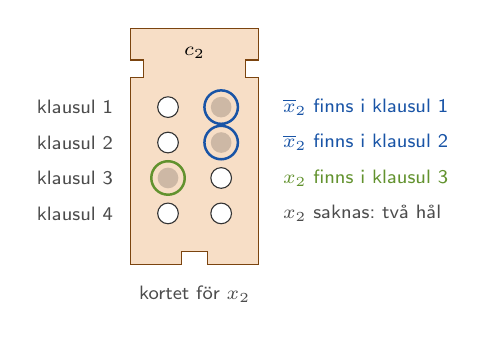
\begin{tikzpicture}[scale=1.25]
        \hkort{0}{0}{0,0,1,0}{1,1,0,0}{$c_2$}{kort}
        \foreach \j/\y in {1/1.60,2/1.24,3/0.88,4/0.52} \node[lab,anchor=east] at (-0.08,\y) {klausul \j};
        \draw[kthblue,line width=0.9pt,visible on=<3->] (0.92,1.60) circle (0.17) (0.92,1.24) circle (0.17);
        \draw[okgreen,line width=0.9pt,visible on=<2->] (0.38,0.88) circle (0.17);
        \node[lab,anchor=west,text=kthblue,visible on=<3->] at (1.45,1.60) {$\xbar{2}$ finns i klausul 1};
        \node[lab,anchor=west,text=kthblue,visible on=<3->] at (1.45,1.24) {$\xbar{2}$ finns i klausul 2};
        \node[lab,anchor=west,text=okgreen,visible on=<2->] at (1.45,0.88) {$x_2$ finns i klausul 3};
        \node[lab,anchor=west,visible on=<4->] at (1.45,0.52) {$x_2$ saknas: två hål};
        \node[lab] at (0.65,-0.3) {kortet för $x_2$};
      \end{tikzpicture}
    \end{column}
  \end{columns}
\end{frame}

\begin{frame}{Exempel: en formel blir fem kort}{Uppgift 3}
  \centering
  {\small $\varphi\;=\;$%
  \alt<2| handout:0>{\textcolor{kthblue}{$\mathbf{(x_1\lor\xbar{2})}$}}{$(x_1\lor\xbar{2})$}$\;\land\;$%
  \alt<3| handout:0>{\textcolor{kthblue}{$\mathbf{(\xbar{1}\lor\xbar{2}\lor\xbar{4})}$}}{$(\xbar{1}\lor\xbar{2}\lor\xbar{4})$}$\;\land\;$%
  \alt<4| handout:0>{\textcolor{kthblue}{$\mathbf{(x_2\lor\xbar{4})}$}}{$(x_2\lor\xbar{4})$}$\;\land\;$%
  \alt<5| handout:0>{\textcolor{kthblue}{$\mathbf{(\xbar{3}\lor x_4)}$}}{$(\xbar{3}\lor x_4)$}}

  \vspace{2mm}
  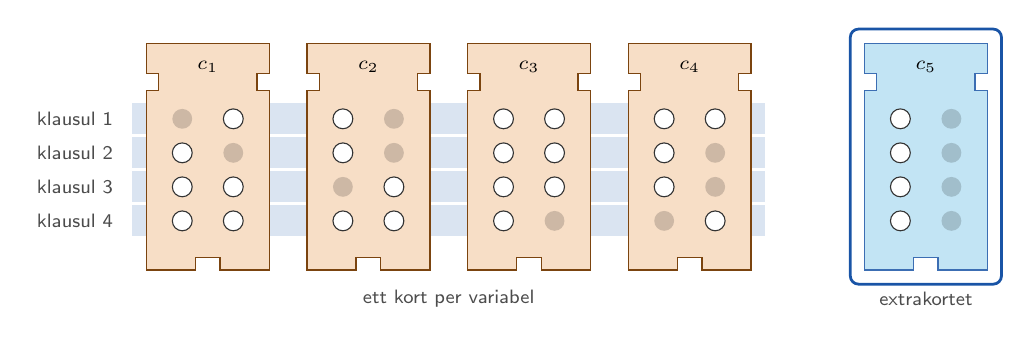
\begin{tikzpicture}[scale=1.2]
    % rad j ligger på höjden 1.96 - 0.36 j
    \fill[kthblue!16,visible on=<2| handout:0>] (-0.15,1.435) rectangle (6.55,1.765);
    \fill[kthblue!16,visible on=<3| handout:0>] (-0.15,1.075) rectangle (6.55,1.405);
    \fill[kthblue!16,visible on=<4| handout:0>] (-0.15,0.715) rectangle (6.55,1.045);
    \fill[kthblue!16,visible on=<5| handout:0>] (-0.15,0.355) rectangle (6.55,0.685);
    \foreach \j/\y in {1/1.60,2/1.24,3/0.88,4/0.52} \node[lab,anchor=east] at (-0.25,\y) {klausul \j};
    \hkort{0}{0}{1,0,0,0}{0,1,0,0}{$c_1$}{kort}
    \hkort{1.7}{0}{0,0,1,0}{1,1,0,0}{$c_2$}{kort}
    \hkort{3.4}{0}{0,0,0,0}{0,0,0,1}{$c_3$}{kort}
    \hkort{5.1}{0}{0,0,0,1}{0,1,1,0}{$c_4$}{kort}
    \hkort{7.6}{0}{0,0,0,0}{1,1,1,1}{$c_5$}{kortextra}
    \draw[kthblue,line width=1pt,rounded corners=3pt,visible on=<6| handout:0>] (7.45,-0.15) rectangle (9.05,2.55);
    \node[lab] at (8.25,-0.3) {extrakortet};
    \node[lab] at (3.2,-0.3) {ett kort per variabel};
  \end{tikzpicture}

  \vspace{1mm}
  \begin{overprint}
    \onslide<1| handout:1>\centering Rad $j$ är klausul $j$. Igenfyllt till vänster: $x_i$ finns i klausulen. Igenfyllt till höger: $\xbar{i}$ finns i klausulen.
    \onslide<2| handout:0>\centering Klausul 1 innehåller $x_1$ och $\xbar{2}$: igenfyllt till vänster på $c_1$ och till höger på $c_2$.
    \onslide<3| handout:0>\centering Klausul 2 innehåller $\xbar{1}$, $\xbar{2}$ och $\xbar{4}$: igenfyllt till höger på $c_1$, $c_2$ och $c_4$.
    \onslide<4| handout:0>\centering Klausul 3 innehåller $x_2$ och $\xbar{4}$: igenfyllt till vänster på $c_2$ och till höger på $c_4$.
    \onslide<5| handout:0>\centering Klausul 4 innehåller $\xbar{3}$ och $x_4$: igenfyllt till höger på $c_3$ och till vänster på $c_4$.
    \onslide<6| handout:0>\centering Extrakortet $c_5$: hål i hela vänsterkolumnen, igenfyllt i hela högerkolumnen.
  \end{overprint}
\end{frame}

\begin{frame}{Exempel: en tilldelning blir en läggning}{Uppgift 3}
  \centering
  {\small $\varphi=(x_1\lor\xbar{2})\land(\xbar{1}\lor\xbar{2}\lor\xbar{4})\land(x_2\lor\xbar{4})\land(\xbar{3}\lor x_4)$ satisfieras av $x_1=1$, $x_2=1$, $x_3=0$, $x_4=0$.}

  \vspace{2mm}
  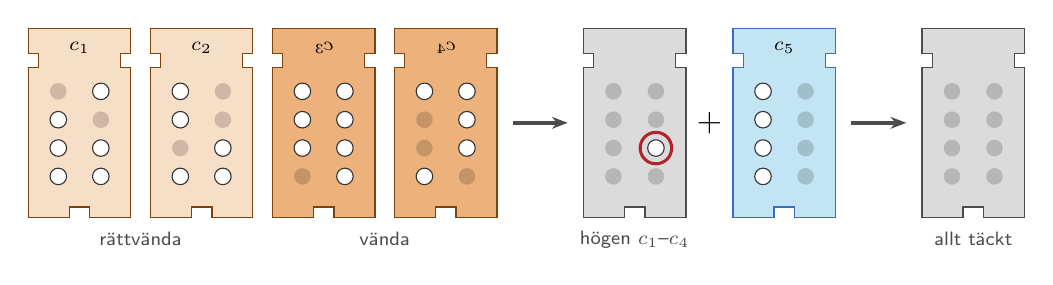
\begin{tikzpicture}[scale=1.0]
    \hkort{0}{0}{1,0,0,0}{0,1,0,0}{$c_1$}{kort}
    \hkort{1.55}{0}{0,0,1,0}{1,1,0,0}{$c_2$}{kort}
    \begin{scope}[visible on=<1| handout:0>]
      \hkort{3.1}{0}{0,0,0,0}{0,0,0,1}{$c_3$}{kort}
      \hkort{4.65}{0}{0,0,0,1}{0,1,1,0}{$c_4$}{kort}
    \end{scope}
    \begin{scope}[visible on=<2->]
      \hkort{3.1}{0}{0,0,0,1}{0,0,0,0}{\spegel{$c_3$}}{kortvand}
      \hkort{4.65}{0}{0,1,1,0}{0,0,0,1}{\spegel{$c_4$}}{kortvand}
      \node[lab] at (4.525,-0.28) {vända};
    \end{scope}
    \node[lab] at (1.425,-0.28) {rättvända};
    \begin{scope}[visible on=<3->]
      \draw[flow,line width=1.2pt] (6.15,1.2) -- (6.85,1.2);
      \hkort{7.05}{0}{1,1,1,1}{1,1,0,1}{}{korthog}
      \node[lab] at (7.7,-0.28) {högen $c_1$--$c_4$};
    \end{scope}
    \draw[badred,line width=1.1pt,visible on=<3| handout:0>] (7.97,0.88) circle (0.2);
    \begin{scope}[visible on=<4->]
      \node[font=\large] at (8.65,1.2) {$+$};
      \hkort{8.95}{0}{0,0,0,0}{1,1,1,1}{$c_5$}{kortextra}
      \draw[flow,line width=1.2pt] (10.45,1.2) -- (11.15,1.2);
      \hkort{11.35}{0}{1,1,1,1}{1,1,1,1}{}{korthog}
      \node[lab] at (12.0,-0.28) {allt täckt};
    \end{scope}
  \end{tikzpicture}

  \vspace{1mm}
  \begin{itemize}
    \item<1-> $x_1=x_2=1$: korten $c_1$ och $c_2$ läggs rättvända.
    \item<2-> $x_3=x_4=0$: korten $c_3$ och $c_4$ vänds. Deras högerkolumner hamnar till vänster.
    \item<3-> I högen är hela vänsterkolumnen täckt. Till höger finns ett hål kvar, på rad 3.
    \item<4-> Extrakortet täpper till högerkolumnen. Pusslet är löst.
  \end{itemize}
\end{frame}

\begin{frame}{Varför behövs extrakortet?}{Uppgift 3}
  \begin{columns}[T]
    \begin{column}{0.64\textwidth}
      \begin{itemize}
        \item<1-> \textbf{Vänster} på rad $j$ täcks av variabelkorten precis när klausul $j$ innehåller en \textbf{sann} literal. Det är vad reglerna är byggda för.
        \item<2-> \textbf{Höger} på rad $j$ täcks av variabelkorten precis när klausul $j$ innehåller en \textbf{falsk} literal. Det är spegelbilden, och den fick vi på köpet.
        \item<3-> Men en satisfierande tilldelning får gärna göra \emph{alla} literaler i en klausul sanna. I exemplet: klausul 3 är $(x_2\lor\xbar{4})$, med $x_2=1$ och $x_4=0$.
        \item<4-> Extrakortet tar bort det oönskade kravet. Rättvänt täcker det hela högerkolumnen och ingenting till vänster.
        \item<5-> Alice Heavey (2019): hålet till höger visar vad den negerade tilldelningen hade gett, och den behöver inte lösa formeln.
      \end{itemize}
    \end{column}
    \begin{column}{0.34\textwidth}
      \centering
      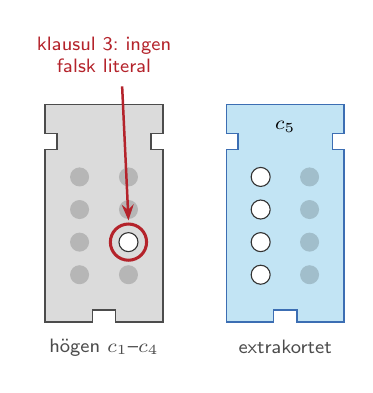
\begin{tikzpicture}[scale=1.15]
        \hkort{0}{0}{1,1,1,1}{1,1,0,1}{}{korthog}
        \node[lab] at (0.65,-0.28) {högen $c_1$--$c_4$};
        \draw[badred,line width=1.1pt,visible on=<3->] (0.92,0.88) circle (0.2);
        \node[lab,text=badred,align=center,visible on=<3->] at (0.65,2.95) {klausul 3: ingen\\falsk literal};
        \draw[badred,-{Stealth[length=2mm]},line width=0.9pt,visible on=<3->] (0.85,2.6) -- (0.92,1.12);
        \begin{scope}[visible on=<4->]
          \hkort{2.0}{0}{0,0,0,0}{1,1,1,1}{$c_5$}{kortextra}
          \node[lab] at (2.65,-0.28) {extrakortet};
        \end{scope}
      \end{tikzpicture}
    \end{column}
  \end{columns}
\end{frame}

\begin{frame}{Korrekthet: $\Rightarrow$ (satisfierbar formel ger lösbart pussel)}{Uppgift 3}
  \begin{columns}[T]
    \begin{column}{0.64\textwidth}
      \textbf{Anta} att $\varphi$ satisfieras av en tilldelning av $x_1,\dots,x_n$.
      \begin{itemize}
        \item<2-> Lägg $c_i$ rättvänt om $x_i=1$ och vänt om $x_i=0$. Lägg extrakortet rättvänt.
        \item<3-> \textbf{Vänsterkolumnen, rad $j$.} Klausul $j$ innehåller en sann literal.
          \begin{itemize}
            \item Är den $x_i$ (alltså $x_i=1$) ligger $c_i$ rättvänt, och dess vänstra hål på rad $j$ är igenfyllt.
            \item Är den $\xbar{i}$ (alltså $x_i=0$) är $c_i$ vänt, och dess igenfyllda högerhål på rad $j$ ligger nu till vänster.
          \end{itemize}
        \item<4-> \textbf{Högerkolumnen.} Extrakortet täcker den helt.
        \item<5-> Alla positioner är täckta. Pusslet $\gamma$ är löst. \hfill$\Box$
      \end{itemize}
    \end{column}
    \begin{column}{0.34\textwidth}
      \centering
      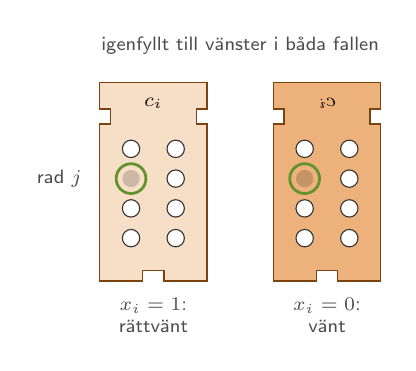
\begin{tikzpicture}[scale=1.05,visible on=<3->]
        \hkort{0}{0}{0,1,0,0}{0,0,0,0}{$c_i$}{kort}
        \draw[okgreen,line width=1pt] (0.38,1.24) circle (0.18);
        \node[lab,align=center] at (0.65,-0.42) {$x_i=1$:\\rättvänt};
        \hkort{2.1}{0}{0,1,0,0}{0,0,0,0}{\spegel{$c_i$}}{kortvand}
        \draw[okgreen,line width=1pt] (2.48,1.24) circle (0.18);
        \node[lab,align=center] at (2.75,-0.42) {$x_i=0$:\\vänt};
        \node[lab,anchor=east] at (-0.1,1.24) {rad $j$};
        \node[lab,align=center] at (1.7,2.85) {igenfyllt till vänster i båda fallen};
      \end{tikzpicture}
    \end{column}
  \end{columns}
\end{frame}

\begin{frame}{Korrekthet: $\Leftarrow$, fall 1 -- extrakortet ligger rättvänt}{Uppgift 3}
  \textbf{Anta} att pusslet $\gamma$ är löst, och att extrakortet ligger rättvänt.
  \begin{itemize}
    \item<2-> Extrakortet täcker ingenting i vänsterkolumnen. Variabelkorten måste alltså täcka den själva.
    \item<3-> Läs av en tilldelning ur läggningen:
      \[x_i=\begin{cases}1 & \text{om } c_i \text{ ligger rättvänt}\\ 0 & \text{annars.}\end{cases}\]
    \item<4-> \textbf{Rad $j$, vänster.} Något kort $c_i$ är igenfyllt där, så som det ligger.
      \begin{itemize}
        \item $c_i$ rättvänt med vänstra hålet igenfyllt: $x_i$ finns i klausul $j$, och $x_i=1$.
        \item $c_i$ vänt med (sitt eget) högra hål igenfyllt: $\xbar{i}$ finns i klausul $j$, och $x_i=0$.
      \end{itemize}
      I båda fallen är klausul $j$ sann.
    \item<5-> Alla $m$ klausuler är sanna. $\varphi$ är satisfierad.
  \end{itemize}
\end{frame}

\begin{frame}{Korrekthet: $\Leftarrow$, fall 2 -- extrakortet ligger vänt}{Uppgift 3}
  \centering
  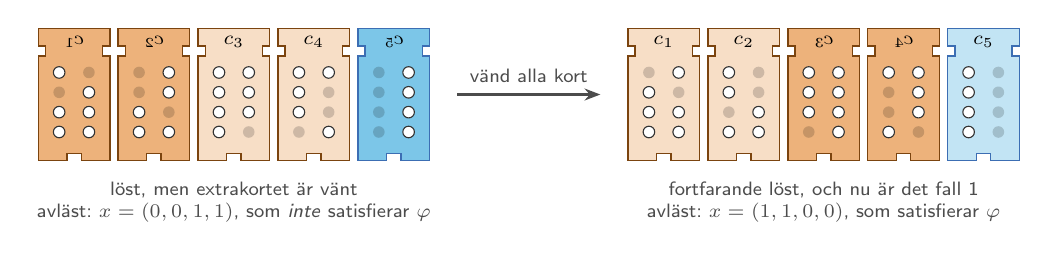
\begin{tikzpicture}[scale=0.7]
    \hkort{0}{0}{0,1,0,0}{1,0,0,0}{\spegel{$c_1$}}{kortvand}
    \hkort{1.45}{0}{1,1,0,0}{0,0,1,0}{\spegel{$c_2$}}{kortvand}
    \hkort{2.9}{0}{0,0,0,0}{0,0,0,1}{$c_3$}{kort}
    \hkort{4.35}{0}{0,0,0,1}{0,1,1,0}{$c_4$}{kort}
    \hkort{5.8}{0}{1,1,1,1}{0,0,0,0}{\spegel{$c_5$}}{kortextravand}
    \node[lab,align=center] at (3.55,-0.75) {löst, men extrakortet är vänt\\avläst: $x=(0,0,1,1)$, som \emph{inte} satisfierar $\varphi$};
    \begin{scope}[visible on=<3->]
      \draw[flow,line width=1.3pt] (7.6,1.2) -- node[above,lab] {vänd alla kort} (10.2,1.2);
      \hkort{10.7}{0}{1,0,0,0}{0,1,0,0}{$c_1$}{kort}
      \hkort{12.15}{0}{0,0,1,0}{1,1,0,0}{$c_2$}{kort}
      \hkort{13.6}{0}{0,0,0,1}{0,0,0,0}{\spegel{$c_3$}}{kortvand}
      \hkort{15.05}{0}{0,1,1,0}{0,0,0,1}{\spegel{$c_4$}}{kortvand}
      \hkort{16.5}{0}{0,0,0,0}{1,1,1,1}{$c_5$}{kortextra}
      \node[lab,align=center] at (14.25,-0.75) {fortfarande löst, och nu är det fall 1\\avläst: $x=(1,1,0,0)$, som satisfierar $\varphi$};
    \end{scope}
  \end{tikzpicture}
  \vspace{1mm}
  \begin{itemize}
    \item<2-> Nu täcker extrakortet hela vänsterkolumnen och ingenting till höger. Variabelkorten har täckt \emph{högerkolumnen}, det vill säga löst den speglade uppgiften.
    \item<3-> \textbf{Vänd hela högen.} Ett löst pussel förblir löst när alla kort vänds: hela bilden speglas, och en täckt botten är täckt också i spegeln.
    \item<4-> Efter vändningen ligger extrakortet rätt, och fall 1 ger en satisfierande tilldelning.
    \item<5-> Uttryckt i variabler: läs av tilldelningen som förut och \textbf{invertera} den. Det är facits formulering -- och svaret på Antons fråga ''vad gör vi om extrakortet är vänt?''. \hfill$\Box$
  \end{itemize}
\end{frame}

\begin{frame}{Polynomisk tid -- och klart}{Uppgift 3}
  \begin{columns}[T]
    \begin{column}{0.58\textwidth}
      \begin{itemize}
        \item<1-> Reduktionen bygger $n+1$ kort med $2m$ positioner var. För varje literal i $\varphi$ fylls ett hål igen. Tid $O(n\cdot m)$.
        \item<2-> Både $n$ och $m$ är högst längden av $\varphi$, så tiden är polynomisk i indatas storlek.
        \item<3-> Vi har visat:
          \begin{enumerate}
            \item \prob{Toys} $\in$ NP,
            \item \prob{Cnf-Sat} $\lep$ \prob{Toys}, med en reduktion som är polynomisk och korrekt åt båda håll.
          \end{enumerate}
        \item<4-> \prob{Toys} är NP-fullständigt.
      \end{itemize}
    \end{column}
    \begin{column}{0.4\textwidth}
      \onslide<4->{
      \begin{block}{Vad var det svåra?}
        Inte beviset. Det svåra var att se att ett kort är en variabel, att en rad är en klausul -- och att spegelbilden behövde ett extra kort för att inte ställa till det.
      \end{block}}
    \end{column}
  \end{columns}
\end{frame}

\begin{frame}{\rabbit vad är pusslet egentligen?}{Uppgift 3}
  \begin{itemize}
    \item<1-> Stryk extrakortet. Då måste variabelkorten täcka \emph{båda} kolumnerna själva.
    \item<2-> Vänster på rad $j$ är täckt $\iff$ klausul $j$ har en sann literal.\\
      Höger på rad $j$ är täckt $\iff$ klausul $j$ har en falsk literal.
    \item<3-> Pusslet utan extrakort är alltså lösbart precis när det finns en tilldelning där varje klausul innehåller \emph{både} en sann och en falsk literal. Det problemet har ett namn: \prob{Not-All-Equal-Sat}, \prob{Nae-Sat}. Det är också NP-fullständigt.
    \item<4-> Det gäller åt båda håll. \emph{Varje} korthög är en \prob{Nae-Sat}-instans: läs av korten rad för rad, igenfyllt till vänster som $x_i$ och igenfyllt till höger som $\xbar{i}$.
    \item<5-> Extrakortet är standardknepet för att reducera \prob{Sat} till \prob{Nae-Sat}: lägg en ny variabel $z$ i varje klausul, här i formen $\overline{z}$. Symmetrin ''vänd alla kort'' är \prob{Nae-Sat}s egen symmetri ''invertera alla variabler''.
    \item<6-> Håstads leksaksaffär säljer alltså \prob{Nae-Sat} i trälåda.
  \end{itemize}
\end{frame}

\begin{frame}{\rabbit lös träpusslet}{Uppgift 3}
  \begin{columns}[T]
    \begin{column}{0.47\textwidth}
      \centering
      \foto{width=\linewidth}{hastad-kort.jpg}\\[2mm]
      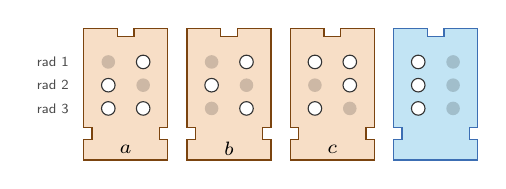
\begin{tikzpicture}[scale=0.82]
        \hkortfoto{0}{0}{1,0,0}{0,1,0}{$a$}{kort}
        \hkortfoto{1.6}{0}{1,0,1}{0,1,0}{$b$}{kort}
        \hkortfoto{3.2}{0}{0,1,0}{0,0,1}{$c$}{kort}
        \hkortfoto{4.8}{0}{0,0,0}{1,1,1}{}{kortextra}
        \foreach \j/\y in {1/1.52,2/1.16,3/0.80} \node[lab,anchor=east,font=\tiny] at (-0.08,\y) {rad \j};
      \end{tikzpicture}
    \end{column}
    \begin{column}{0.51\textwidth}
      \begin{itemize}
        \item<1-> Det fjärde kortet har hål i bara en kolumn. Det är extrakortet, och kolumnen med hålen är den vi kallar vänster.
        \item<2-> Läs av rad för rad. Igenfyllt till vänster: variabeln. Igenfyllt till höger: negationen.
          \begin{itemize}
            \item rad 1: $a$ och $b$
            \item rad 2: $\overline{a}$, $\overline{b}$ och $c$
            \item rad 3: $b$ och $\overline{c}$
          \end{itemize}
        \item<3-> $\varphi=(a\lor b)\land(\overline{a}\lor\overline{b}\lor c)\land(b\lor\overline{c})$
        \item<4-> Fyra tilldelningar satisfierar $\varphi$. Den enklaste är $a=b=c=1$: lägg korten precis som de ligger på fotot. Vill man vända på något: $a=0$, $b=1$, $c=0$ går också.
      \end{itemize}
    \end{column}
  \end{columns}
\end{frame}

\begin{frame}{\rabbit småfrågor från bakersta raden}{Uppgift 3}
  \begin{itemize}
    \item<1-> \textbf{Spelar ordningen i högen någon roll?} Nej. En position är täckt om \emph{något} kort är igenfyllt där.
    \item<2-> \textbf{Kan $x_i$ och $\xbar{i}$ stå i samma klausul?} Ja. Då är båda hålen igenfyllda på den raden av $c_i$, och raden är täckt hur kortet än ligger. Klausulen är också sann hur $x_i$ än väljs. Det stämmer.
    \item<3-> \textbf{En tom klausul?} Då har inget variabelkort något igenfyllt hål på den raden, och extrakortet täcker bara den ena sidan. Pusslet går inte att lösa, och formeln är inte satisfierbar. Det stämmer också.
    \item<4-> \textbf{Varför \prob{Cnf-Sat} och inte \prob{3-Cnf-Sat}?} Båda duger. Reduktionen bryr sig inte om hur många literaler en klausul har, och \prob{3-Cnf-Sat} är ett specialfall.
    \item<5-> \textbf{Var kommer pusslet ifrån?} Det är en klassiker. Samma uppgift finns under namnet \prob{Puzzle} i Sipsers lärobok \emph{Introduction to the Theory of Computation}.
  \end{itemize}
\end{frame}

% ===================== del6-schema.tex =====================
\section{Uppgift 4: Processorschemaläggning}

\begin{frame}{Uppgift 4: Processorschemaläggning}{uppgiften i repris}
  \uppgiftFyra
\end{frame}

\begin{frame}{Rita problemet: konfliktgrafen}{Uppgift 4}
  \begin{columns}[T]
    \begin{column}{0.5\textwidth}
      \begin{itemize}
        \item<1-> Låt varje jobb vara ett hörn.
        \item<1-> Låt varje villkor ''jobb $i$ inte samtidigt som jobb $j$'' vara en kant mellan $i$ och $j$.
        \item<2-> Ett schema ger varje jobb en tidsenhet. Två jobb med ett villkor mellan sig måste få olika.
        \item<3-> Byt ordet ''tidsenhet'' mot ''färg'' och läs meningen igen.
        \item<4-> Ett schema på tre tidsenheter \emph{är} en trefärgning av konfliktgrafen. Processorerna spelar ingen roll: det finns alltid tillräckligt många.
      \end{itemize}
    \end{column}
    \begin{column}{0.48\textwidth}
      \centering
      \begin{tikzpicture}
        \node[bx,minimum width=9mm,alt=<2->{t1}{}] (j1) at (0,1.1) {$J_1$};
        \node[bx,minimum width=9mm,alt=<2->{t2}{}] (j2) at (1.6,1.9) {$J_2$};
        \node[bx,minimum width=9mm,alt=<2->{t3}{}] (j3) at (1.6,0.3) {$J_3$};
        \node[bx,minimum width=9mm,alt=<2->{t1}{}] (j4) at (3.2,1.9) {$J_4$};
        \node[bx,minimum width=9mm,alt=<2->{t2}{}] (j5) at (3.2,0.3) {$J_5$};
        \begin{scope}[on background layer]
          \draw[badred,line width=1pt,densely dashed] (j1) -- (j2) -- (j3) -- (j1) (j2) -- (j4) -- (j5) -- (j3);
        \end{scope}
        % tidsaxeln
        \foreach \t in {1,2,3} {
          \draw[black!60] (\t*1.45-1.75,-2.5) rectangle (\t*1.45-0.45,-0.75);
          \node[lab] at (\t*1.45-1.1,-2.75) {tid \t};
        }
        \node[bx,t1,minimum width=9mm,minimum height=6mm,visible on=<2->] at (0.35,-1.2) {$J_1$};
        \node[bx,t1,minimum width=9mm,minimum height=6mm,visible on=<2->] at (0.35,-2.0) {$J_4$};
        \node[bx,t2,minimum width=9mm,minimum height=6mm,visible on=<2->] at (1.8,-1.2) {$J_2$};
        \node[bx,t2,minimum width=9mm,minimum height=6mm,visible on=<2->] at (1.8,-2.0) {$J_5$};
        \node[bx,t3,minimum width=9mm,minimum height=6mm,visible on=<2->] at (3.25,-1.2) {$J_3$};
      \end{tikzpicture}
    \end{column}
  \end{columns}
\end{frame}

\begin{frame}{Steg 1: \prob{Schedule} ligger i NP}{Uppgift 4}
  \begin{itemize}
    \item<1-> Lisa Lis bilder (2019) lämnar det här steget som egen övning. Här är den.
    \item<2-> \textbf{Lösning (certifikat):} ett schema, det vill säga en tidsenhet $t(i)\in\{1,2,3\}$ för varje jobb $i$.
    \item<3-> \textbf{Verifiera:}
      \begin{enumerate}
        \item[a)] varje jobb har fått precis en tidsenhet mellan 1 och 3,
        \item[b)] för varje villkor $(i,j)$ gäller $t(i)\neq t(j)$.
      \end{enumerate}
    \item<4-> \textbf{Tid:} $O(n + \text{antalet villkor})$. Linjärt i indatas storlek.
    \item<5-> Vi behöver aldrig kontrollera att processorerna räcker. Uppgiften lovar att de gör det, och $n$ stycken räcker alltid.
  \end{itemize}
\end{frame}

\begin{frame}[fragile]{Steg 2: reducera \prob{3-färgning}}{Uppgift 4}
  \begin{columns}[T]
    \begin{column}{0.6\textwidth}
\begin{lstlisting}
function 3-färgning(G = (V, E))
    foreach v in V do
        skapa ett jobb v
    foreach (u, v) in E do
        skapa villkoret "u inte samtidigt som v"
    return Schedule(jobben, villkoren)
\end{lstlisting}
      \begin{itemize}
        \item<2-> \prob{3-färgning} är känt NP-fullständigt, och det är dessutom samma problem som vårt. Det är ett bra val.
        \item<3-> Ett anrop, svaret returneras direkt: en karpreduktion.
        \item<4-> Reduktionen går igenom varje hörn och varje kant en gång: $O(|V|+|E|)$.
      \end{itemize}
    \end{column}
    \begin{column}{0.38\textwidth}
      \centering
      \begin{tikzpicture}
        \node[bx,fill=kthblue!12,minimum width=34mm] (B) at (0,2.4) {\prob{3-färgning}\\{\scriptsize känt NP-fullständigt}};
        \node[bx,fill=warnorange!18,minimum width=34mm] (A) at (0,0) {\prob{Schedule}\\{\scriptsize vårt problem}};
        \draw[flow,line width=1.5pt,kthblue] (B) -- node[right,font=\small,align=left] {hörn $\mapsto$ jobb\\kant $\mapsto$ villkor\\färg $\mapsto$ tidsenhet} (A);
      \end{tikzpicture}
    \end{column}
  \end{columns}
\end{frame}

\begin{frame}{Exempel: sju hörn blir sju jobb}{Uppgift 4}
  \centering
  \begin{tikzpicture}
    % grafen
    \coordinate (n1) at (0,0); \coordinate (n2) at (1.3,0.95); \coordinate (n3) at (1.3,-0.95);
    \coordinate (n4) at (2.8,0.95); \coordinate (n5) at (2.8,-0.95); \coordinate (n6) at (4.1,0); \coordinate (n7) at (2.8,-2.2);
    \draw[ed] (n1) -- (n2) -- (n3) -- (n1) (n2) -- (n4) -- (n5) -- (n3) (n4) -- (n6) -- (n5) (n6) -- (n7) -- (n3);
    \node[vx,alt=<2->{t1}{}] at (n1) {1};
    \node[vx,alt=<2->{t2}{}] at (n2) {2};
    \node[vx,alt=<2->{t3}{}] at (n3) {3};
    \node[vx,alt=<2->{t1}{}] at (n4) {4};
    \node[vx,alt=<2->{t2}{}] at (n5) {5};
    \node[vx,alt=<2->{t3}{}] at (n6) {6};
    \node[vx,alt=<2->{t1}{}] at (n7) {7};
    \node[lab,align=center] at (2.0,1.75) {grafen $G$: 7 hörn, 10 kanter};
    % pilen
    \draw[flow,line width=1.3pt,visible on=<3->] (4.9,-0.6) -- node[above,lab] {reduktion} (6.3,-0.6);
    % schemat
    \foreach \t in {1,2,3} {
      \draw[black!60,visible on=<3->] (\t*1.45+5.35,-2.45) rectangle (\t*1.45+6.65,0.95);
      \node[lab,visible on=<3->] at (\t*1.45+6.0,-2.7) {tid \t};
    }
    \node[lab,visible on=<3->] at (8.9,1.75) {schemat: 7 jobb, 10 villkor, 3 tidsenheter};
    \foreach \j/\y in {1/0.45,4/-0.35,7/-1.15} \node[bx,t1,minimum width=10mm,minimum height=6mm,visible on=<3->] at (7.45,\y) {jobb \j};
    \foreach \j/\y in {2/0.45,5/-0.35} \node[bx,t2,minimum width=10mm,minimum height=6mm,visible on=<3->] at (8.9,\y) {jobb \j};
    \foreach \j/\y in {3/0.45,6/-0.35} \node[bx,t3,minimum width=10mm,minimum height=6mm,visible on=<3->] at (10.35,\y) {jobb \j};
  \end{tikzpicture}
  \begin{itemize}
    \item<2-> En trefärgning: hörnen 1, 4 och 7 får färg 1; hörnen 2 och 5 färg 2; hörnen 3 och 6 färg 3.
    \item<3-> Samma sak som schema: jobben 1, 4 och 7 körs under tidsenhet 1, och så vidare. Inga två jobb i samma kolumn har ett villkor mellan sig.
    \item<4-> Två tidsenheter räcker inte: hörnen 1, 2 och 3 bildar en triangel.
  \end{itemize}
\end{frame}

\begin{frame}{Korrekthet: en trefärgning är ett schema, och omvänt}{Uppgift 4}
  \begin{columns}[T]
    \begin{column}{0.48\textwidth}
      \begin{block}{$\Rightarrow$\ \ $G$ trefärgbar ger schema på 3 tidsenheter}
        \begin{itemize}
          \item Ta en trefärgning och låt $C_i$ vara hörnen med färg $i$.
          \item<2-> Det finns inga kanter inom $C_i$, alltså inga villkor mellan jobben i $C_i$.
          \item<3-> Kör alla jobb i $C_1$ under tidsenhet 1, alla i $C_2$ under tidsenhet 2 och alla i $C_3$ under tidsenhet 3.
        \end{itemize}
      \end{block}
    \end{column}
    \begin{column}{0.48\textwidth}
      \onslide<4->{
      \begin{block}{$\Leftarrow$\ \ schema på 3 tidsenheter ger trefärgning}
        \begin{itemize}
          \item Ge hörnet $v$ färg $i$ om jobbet $v$ körs under tidsenhet $i$.
          \item<5-> Två grannar har ett villkor mellan sig. Deras jobb körs alltså under olika tidsenheter, och hörnen får olika färg.
          \item<6-> Det är en giltig trefärgning.
        \end{itemize}
      \end{block}}
    \end{column}
  \end{columns}
  \onslide<7->{
  \vspace{2mm}
  \prob{Schedule} ligger i NP och \prob{3-färgning} $\lep$ \prob{Schedule}. Alltså är \prob{Schedule} NP-fullständigt. \hfill$\Box$

  \smallskip
  {\small Beviset är kort eftersom reduktionen inte gör något. De två problemen är samma problem i olika kläder.}}
\end{frame}

\begin{frame}{b) Fler tidsenheter: $k>3$}{Uppgift 4}
  \begin{columns}[T]
    \begin{column}{0.58\textwidth}
      \begin{itemize}
        \item<1-> \textbf{Facit:} med samma argument kan \prob{$k$-färgning} reduceras till \prob{Schedule} med $k$ tidsenheter. Alltså NP-fullständigt för varje $k\ge3$.
        \item<2-> Det förutsätter att \prob{$k$-färgning} är NP-fullständigt för varje fast $k\ge3$. Är det det?
        \item<3-> \textbf{Direkt variant:} reducera \prob{3-färgning} igen, men lägg till $k-3$ \emph{blockerarjobb} $z_1,\dots,z_{k-3}$ med villkor mot alla andra jobb, och mot varandra.
        \item<4-> Varje blockerare tvingas ensam in i en egen tidsenhet. Kvar till grafens jobb blir precis tre.
        \item<5-> $G$ trefärgbar $\iff$ jobben går på $k$ tidsenheter. Samma knep, med en klick på $k-3$ hörn, ger att \prob{$k$-färgning} är NP-fullständigt.
      \end{itemize}
    \end{column}
    \begin{column}{0.4\textwidth}
      \centering
      \onslide<3->{%
      \begin{tikzpicture}[scale=0.95]
        \draw[kthblue,fill=kthblue!8] (0,0) ellipse (1.5 and 1.0);
        \node[font=\small] at (0,0.1) {jobben från $G$};
        \node[lab] at (0,-0.4) {(hörnen)};
        \node[bx,t4,minimum width=8mm] (z1) at (3.0,0.7) {$z_1$};
        \node[bx,t4,minimum width=8mm] (z2) at (3.0,-0.7) {$z_2$};
        \draw[badred,line width=2.2pt,densely dashed] (1.42,0.3) -- (z1.west);
        \draw[badred,line width=2.2pt,densely dashed] (1.42,-0.3) -- (z2.west);
        \draw[badred,line width=1pt,densely dashed] (z1) -- (z2);
        \node[lab,text=badred,align=center] at (1.6,1.45) {villkor mot \emph{alla}};
        % tidsaxel för k = 5
        \foreach \t/\st/\txt in {1/t1/,2/t2/,3/t3/,4/t4/$z_1$,5/t4/$z_2$} {
          \node[draw=black!60,\st,minimum width=9.5mm,minimum height=8mm,font=\small] at (\t*1.0-1.9,-2.3) {\txt};
          \node[lab] at (\t*1.0-1.9,-2.95) {tid \t};
        }
        \draw[decorate,decoration={brace,amplitude=3pt},black!60] (-1.4,-1.8) -- (1.6,-1.8) node[midway,above=3pt,lab] {grafens jobb};
        \node[lab] at (1.1,-3.45) {exempel: $k=5$, två blockerare};
      \end{tikzpicture}}
    \end{column}
  \end{columns}
\end{frame}

\begin{frame}[fragile]{c) Två tidsenheter: $k=2$}{Uppgift 4}
  \begin{columns}[T]
    \begin{column}{0.62\textwidth}
      Nu vänder vi på reduktionen och \emph{löser} problemet: bygg konfliktgrafen och försök tvåfärga den.
\begin{lstlisting}
function Schedule2(jobb, villkor)
    foreach jobb s utan tid do
        tid[s] <- 1;  lägg s i kön
        while kön inte är tom do
            u <- ta ut ett jobb ur kön
            foreach villkor (u, v) do
                if v saknar tid then
                    tid[v] <- 3 - tid[u];  lägg v i kön
                else if tid[v] = tid[u] then
                    return nej
    return ja
\end{lstlisting}
      \begin{itemize}
        \item<2-> Har ett jobb tid 1 måste alla dess grannar ha tid 2, och tvärtom. Inget val finns att göra.
        \item<3-> Bredden-först-sökning (facit tar djupet-först, det går lika bra): $O(n+\text{antalet villkor})$. Problemet ligger i P.
      \end{itemize}
    \end{column}
    \begin{column}{0.36\textwidth}
      \centering
      \begin{tikzpicture}
        \foreach \k in {0,...,4} \coordinate (o\k) at (\k*72+90:1.25);
        \draw[ed] (o0) -- (o1) -- (o2) -- (o3) -- (o4);
        \draw[alt=<2->{badred,line width=1.6pt}{ed}] (o4) -- (o0);
        \node[vx,alt=<2->{t1}{}] at (o0) {1};
        \node[vx,alt=<2->{t2}{}] at (o1) {2};
        \node[vx,alt=<2->{t1}{}] at (o2) {3};
        \node[vx,alt=<2->{t2}{}] at (o3) {4};
        \node[vx,alt=<2->{fill=badred!30}{}] at (o4) {5};
        \node[lab,align=center,visible on=<2->] at (0,-2.05) {tider 1, 2, 1, 2 -- och jobb 5 krockar\\med både jobb 4 och jobb 1};
        \node[lab,align=center,visible on=<3->] at (0,-2.9) {udda cykel: går inte på två tidsenheter.\\Utan udda cykler går det alltid\\(grafen är bipartit).};
      \end{tikzpicture}
    \end{column}
  \end{columns}
\end{frame}

\begin{frame}{Samma översättning, motsatt håll, motsatt slutsats}{Uppgift 4}
  \centering
  \begin{tabular}{@{}L{1.6cm}L{4.8cm}L{6.2cm}@{}}
    \toprule
     & \textbf{Reduktion} & \textbf{Vad den visar} \\
    \midrule
    $k=3$ & \prob{3-färgning} $\lep$ \prob{Schedule} & \prob{Schedule} är minst lika svårt som \prob{3-färgning}: NP-svårt \\[2mm]
    $k=2$ & \prob{Schedule$_2$} $\lep$ \prob{2-färgning} & \prob{Schedule$_2$} är inte svårare än \prob{2-färgning}: ligger i P \\
    \bottomrule
  \end{tabular}
  \vspace{3mm}
  \begin{itemize}
    \item<2-> Översättningen är densamma i båda fallen: jobb är hörn, villkor är kanter.
    \item<3-> För att visa att ett problem är \textbf{svårt} reducerar man ett svårt problem \emph{till} det.
    \item<4-> För att visa att ett problem är \textbf{lätt} reducerar man det till ett lätt problem. Det kallas vanligen att skriva en algoritm.
    \item<5-> Den som i tentasalen skriver ''vi reducerar \prob{Schedule} till \prob{3-färgning}, alltså är \prob{Schedule} NP-svårt'' har visat att \prob{Schedule} ligger i NP. Det är också sant, men det var inte det som skulle visas.
  \end{itemize}
\end{frame}

\begin{frame}{\rabbit är problemet NP-fullständigt för $k=2$?}{Uppgift 4}
  \begin{itemize}
    \item<1-> Uppgiftens svar: \textbf{nej}. Med två tidsenheter löses problemet på linjär tid.
    \item<2-> Pedantens svar: nej, \emph{såvida inte $\mathrm{P}=\mathrm{NP}$}.
    \item<3-> Om $\mathrm{P}=\mathrm{NP}$ är nämligen varje problem i P NP-fullständigt, utom de två som alltid svarar ja respektive alltid svarar nej. Reduktionen från ett godtyckligt problem i NP: lös instansen på polynomisk tid, och skriv sedan ut en fix ja-instans eller en fix nej-instans.
    \item<4-> Därför säger en försiktig teoretiker ''ligger i P'' och inte ''är inte NP-fullständigt''.
    \item<5-> Och $k=1$? Alla jobb körs samtidigt. Svaret är ja precis när det inte finns några villkor alls.
  \end{itemize}
  \onslide<6->{
  \vspace{2mm}
  \centering
  \begin{tikzpicture}
    \draw[flow,black!60] (0,0) -- (11.5,0) node[right,lab] {$k$};
    \foreach \x/\k in {1.5/1,4.0/2,6.5/3,9.0/4} { \draw[black!60] (\x,0.1) -- (\x,-0.1); \node[lab,below] at (\x,-0.1) {$k=\k$}; }
    \node[bx,fill=okgreen!20,font=\scriptsize] at (1.5,0.6) {trivialt};
    \node[bx,fill=okgreen!20,font=\scriptsize] at (4.0,0.6) {linjär tid (BFS)};
    \node[bx,fill=badred!15,font=\scriptsize,minimum width=40mm] at (8.0,0.6) {NP-fullständigt för varje $k\ge3$};
  \end{tikzpicture}}
\end{frame}

\begin{frame}{\rabbit tänk om processorerna tar slut?}{Uppgift 4}
  \begin{columns}[T]
    \begin{column}{0.6\textwidth}
      \begin{itemize}
        \item<1-> Uppgiften lovar ''ett tillräckligt antal processorer''. Anta i stället att det finns $p$ stycken: högst $p$ jobb per tidsenhet.
        \item<2-> $k=3$: fortfarande NP-fullständigt, förstås.
        \item<3-> $k=2$: tvåfärga varje sammanhängande del av konfliktgrafen för sig. Del $i$ har två sidor, med $a_i$ och $b_i$ jobb, och får vändas fritt.
        \item<4-> Välj en sida per del så att högst $p$ jobb hamnar i varje tidsenhet. Det är en delmängdssumma!
        \item<5-> Men talen $a_i$ och $b_i$ är högst $n$. De \emph{räknar} saker i indata i stället för att stå skrivna där. Dynamisk programmering över ''antal jobb i tidsenhet 1'' tar $O(n^2)$, polynomiskt på riktigt.
      \end{itemize}
    \end{column}
    \begin{column}{0.38\textwidth}
      \centering
      \onslide<3->{%
      \begin{tikzpicture}
        % del A: stjärna 1|3
        \coordinate (a0) at (0,0); \coordinate (a1) at (-0.7,-1.0); \coordinate (a2) at (0,-1.0); \coordinate (a3) at (0.7,-1.0);
        \draw[ed] (a0) -- (a1) (a0) -- (a2) (a0) -- (a3);
        \node[vx,t2,minimum size=4.5mm] at (a0) {};
        \foreach \k in {1,2,3} \node[vx,t1,minimum size=4.5mm] at (a\k) {};
        \node[lab] at (0,-1.6) {$3\,|\,1$};
        % del B: stig 1|2
        \coordinate (b0) at (1.9,0); \coordinate (b1) at (1.55,-1.0); \coordinate (b2) at (2.25,-1.0);
        \draw[ed] (b1) -- (b0) -- (b2);
        \node[vx,t1,minimum size=4.5mm] at (b0) {};
        \node[vx,t2,minimum size=4.5mm] at (b1) {};
        \node[vx,t2,minimum size=4.5mm] at (b2) {};
        \node[lab] at (1.9,-1.6) {$1\,|\,2$};
        % del C: ensamt jobb
        \node[vx,t2,minimum size=4.5mm] at (3.3,-0.5) {};
        \node[lab] at (3.3,-1.6) {$0\,|\,1$};
        \node[lab,align=center] at (1.6,0.75) {tre delar, $n=8$ jobb, $p=4$ processorer};
        \node[bx,t1,font=\scriptsize,minimum width=24mm] at (0.4,-2.55) {tid 1: $3+1+0=4$};
        \node[bx,t2,font=\scriptsize,minimum width=24mm] at (3.0,-2.55) {tid 2: $1+2+1=4$};
      \end{tikzpicture}}
      \onslide<5->{

      \vspace{2mm}
      {\small Pseudopolynomiskt är bara ett problem när talen står i indata.}}
    \end{column}
  \end{columns}
\end{frame}

\begin{frame}{\rabbit samma problem i andra kläder}{Uppgift 4}
  \begin{columns}[T]
    \begin{column}{0.62\textwidth}
      \begin{itemize}
        \item<1-> \textbf{Tentaschema:} kurser är jobb, en gemensam student är ett villkor, tentatillfällen är tidsenheter.
        \item<2-> \textbf{Registerallokering i kompilatorer:} variabler är hörn, två variabler som lever samtidigt har en kant, processorns register är färger. (Chaitin m.fl., tidigt 1980-tal.)
        \item<3-> \textbf{Frekvenstilldelning:} sändare är hörn, sändare som stör varandra har en kant, frekvenser är färger.
        \item<4-> \textbf{Sudoku:} 81 hörn, nio färger, och några hörn färdigfärgade av tidningen.
        \item<5-> Det är samma NP-fullständiga problem varje gång. Namnet byts. Svårigheten består.
      \end{itemize}
    \end{column}
    \begin{column}{0.36\textwidth}
      \onslide<5->{
      \begin{block}{Praktisk nytta}
        Känner du igen ditt problem som graffärgning vet du två saker: att det finns färdiga heuristiker, och att du inte ska lova chefen en snabb exakt algoritm.
      \end{block}}
    \end{column}
  \end{columns}
\end{frame}

% ===================== del7-lapptacke.tex =====================
\section{Uppgift 5: Lapptäcke}

\begin{frame}{Uppgift 5: Lapptäcke}{uppgiften i repris}
  \uppgiftFem
\end{frame}

\begin{frame}{Formulering med matematisk notation}{Uppgift 5}
  \begin{columns}[T]
    \begin{column}{0.58\textwidth}
      \textbf{Indata} till konstruktionsproblemet \prob{LK}:
      \begin{itemize}
        \item en lista med talpar $(b_i,h_i)$, $1\le i\le n$: bredd och höjd på lapp $i$,
        \item två tal $B$ och $H$: täckets bredd och höjd.
      \end{itemize}
      Samtliga tal är positiva heltal.

      \smallskip
      \onslide<2->{\textbf{Lösning:} en lista med fyrtupler $(l_i,x_i,y_i,v_i)$, där
      \begin{itemize}
        \item $l_i\in\{1,\dots,n\}$ är numret på en lapp,
        \item $(x_i,y_i)$ är var lappens nedre vänstra hörn ska ligga,
        \item $v_i$ är en boolesk variabel som anger om lappen ska vridas.
      \end{itemize}}
      \onslide<3->{\textbf{Villkor:} lapparna får inte överlappa och måste täcka samtliga punkter $(x,y)$ med $0\le x<B$ och $0\le y<H$. Inga andra punkter får täckas.}
    \end{column}
    \begin{column}{0.4\textwidth}
      \centering
      \begin{tikzpicture}[x=8mm,y=8mm]
        \draw[lapp,fill=kthblue!25] (0,0) rectangle +(3,2); \node[font=\scriptsize] at (1.5,1) {lapp 1};
        \draw[lapp,fill=okgreen!30] (3,0) rectangle +(2,2); \node[font=\scriptsize] at (4,1) {lapp 2};
        \draw[lapp,fill=warnorange!35] (0,2) rectangle +(2,1); \node[font=\scriptsize] at (1,2.5) {lapp 3};
        \draw[lapp,fill=kthsky!35] (2,2) rectangle +(3,1); \node[font=\scriptsize] at (3.5,2.5) {lapp 4, vriden};
        \draw[black,line width=1.1pt] (0,0) rectangle (5,3);
        \draw[flow] (0,0) -- (5.7,0) node[right,lab] {$x$};
        \draw[flow] (0,0) -- (0,3.7) node[above,lab] {$y$};
        \foreach \x in {0,...,5} \node[lab,below] at (\x,-0.05) {\x};
        \foreach \y in {1,2,3} \node[lab,left] at (-0.05,\y) {\y};
        \node[circle,fill=badred,inner sep=1.6pt,visible on=<2->] at (2,2) {};
        \draw[badred,-{Stealth[length=2mm]},visible on=<2->] (2.9,4.1) -- (2.07,2.12);
        \node[lab,text=badred,anchor=west,visible on=<2->] at (2.9,4.15) {$(x_4,y_4)=(2,2)$};
      \end{tikzpicture}

      \onslide<2->{\scriptsize
      \begin{tabular}{@{}ll@{}}
        indata: & $(3,2),\,(2,2),\,(2,1),\,(1,3),\,(2,3)$\\
         & $B=5$,\ $H=3$\\
        lösning: & $(1,0,0,\text{nej}),\ (2,3,0,\text{nej}),$\\
         & $(3,0,2,\text{nej}),\ (4,2,2,\text{ja})$
      \end{tabular}}
    \end{column}
  \end{columns}
\end{frame}

\begin{frame}{Beslutsproblemet och planen}{Uppgift 5}
  \begin{columns}[T]
    \begin{column}{0.58\textwidth}
      \begin{itemize}
        \item<1-> \prob{LK}: \emph{konstruera} ett lapptäcke (eller säg att inget finns).
        \item<1-> \prob{LB}: \emph{finns} det en lösning till \prob{LK}? Ja eller nej.
        \item<2-> För att visa att \prob{LB} är NP-fullständigt visar vi
          \begin{enumerate}
            \item att \prob{LB} ligger i NP,
            \item att \prob{Delmängdssumma}, ett känt NP-fullständigt problem, kan reduceras till \prob{LB}.
          \end{enumerate}
        \item<3-> Steg 1 ser oskyldigt ut. Det är där fällan ligger.
      \end{itemize}
    \end{column}
    \begin{column}{0.4\textwidth}
      \onslide<4->{
      \begin{block}{En randanmärkning}
        Uppgiften säger ''konstruktionsoptimeringsproblem'', men här finns ingen målfunktion. Varje täcke av rätt storlek duger; inget är bättre än något annat.

        \smallskip
        Det gör ingenting. Vi ska ändå bara bevisa något om beslutsproblemet.
      \end{block}}
    \end{column}
  \end{columns}
\end{frame}

\begin{frame}{Steg 1, första försöket: rita upp täcket}{Uppgift 5}
  \begin{columns}[T]
    \begin{column}{0.6\textwidth}
      \begin{itemize}
        \item<1-> Naturlig idé: gör en $B\times H$-matris med en ruta per kvadratmillimeter. Gå igenom lapparna en i taget och markera rutorna de täcker.
        \item<2-> En ruta som redan är tagen: överlapp. En lapp utanför matrisen: utanför täcket. En omarkerad ruta på slutet: hål.
        \item<3-> Lätt att programmera, uppenbart korrekt.
        \item<4-> Och \textbf{pseudopolynomiskt}. Matrisen har $B\cdot H$ rutor, och det är exponentiellt många i indatas längd.
        \item<5-> Det hjälper inte om matrisen är själva certifikatet (Lisa Li, 2019) eller något verifieraren ritar själv (Alice Heavey, 2019). För stor är den ändå.
      \end{itemize}
    \end{column}
    \begin{column}{0.38\textwidth}
      \centering
      \begin{tikzpicture}[x=6.5mm,y=6.5mm]
        \fill[kthblue!25] (0,0) rectangle (3,2);
        \fill[okgreen!30] (3,0) rectangle (5,2);
        \fill[warnorange!35] (0,2) rectangle (2,3);
        \fill[kthsky!35,visible on=<1| handout:0>] (2,2) rectangle (5,3);
        \fill[kthsky!35,visible on=<2->] (2,2) rectangle (4,3);
        \draw[step=1,black!45] (0,0) grid (5,3);
        \draw[black,line width=1pt] (0,0) rectangle (5,3);
        \foreach \x/\y in {0/0,1/0,2/0,0/1,1/1,2/1} \node[font=\tiny] at (\x+0.5,\y+0.5) {1};
        \foreach \x/\y in {3/0,4/0,3/1,4/1} \node[font=\tiny] at (\x+0.5,\y+0.5) {2};
        \foreach \x/\y in {0/2,1/2} \node[font=\tiny] at (\x+0.5,\y+0.5) {3};
        \foreach \x/\y in {2/2,3/2} \node[font=\tiny] at (\x+0.5,\y+0.5) {4};
        \node[font=\tiny,visible on=<1| handout:0>] at (4.5,2.5) {4};
        \node[font=\scriptsize\bfseries,text=badred,visible on=<2->] at (4.5,2.5) {?};
        \node[lab,align=center] at (2.5,-0.75) {matrisen för ett $5\times3$-täcke:\\15 rutor, ett lappnummer i varje};
        \node[lab,text=badred,align=center,visible on=<2->] at (2.5,3.6) {en omarkerad ruta: hål};
      \end{tikzpicture}
    \end{column}
  \end{columns}
\end{frame}

\begin{frame}{Hur stort är täcket egentligen?}{Uppgift 5}
  \begin{columns}[T]
    \begin{column}{0.5\textwidth}
      \centering
      \begin{tabular}{@{}rrr@{}}
        \toprule
        bredd = höjd & bitar & rutor i matrisen\\
        \midrule
        1 & 2 & 1\\
        10 & 8 & 100\\
        100 & 14 & 10\,000\\
        1\,000 & 20 & 1\,000\,000\\
        10\,000 & 28 & 100\,000\,000\\
        100\,000 & 34 & 10\,000\,000\,000\\
        \midrule
        $10^{9}$ & 60 & $10^{18}$\\
        \bottomrule
      \end{tabular}

      \vspace{1mm}
      {\scriptsize\textcolor{softgray}{Mått i millimeter. Bitar: bredd och höjd tillsammans.\\De sex första raderna är Alice Heaveys tabell (2019).}}
    \end{column}
    \begin{column}{0.48\textwidth}
      \begin{itemize}
        \item<2-> Talen $B$ och $H$ skrivs med $\log B+\log H$ bitar.
        \item<3-> Matrisen har $B\cdot H=2^{\log B+\log H}$ rutor.
        \item<4-> Kvadratiskt i \emph{talen} i indata. Exponentiellt i indatas \emph{längd}.
        \item<5-> En siffra till i bredden och en till i höjden gör täcket hundra gånger större.
        \item<6-> Sista raden är ett lapptäcke på 1000 km gånger 1000 km. Det beskrivs med 60 bitar och har en triljon rutor. Ingen hinner pricka av dem.
      \end{itemize}
    \end{column}
  \end{columns}
\end{frame}

\begin{frame}{Steg 1, andra försöket: räkna i stället för att rita}{Uppgift 5}
  \textbf{Lösning (certifikat):} listan $(l_i,x_i,y_i,v_i)$ från formuleringen. Högst $n$ lappar, och varje tal ryms i lika många bitar som $B$ eller $H$. Certifikatet är alltså polynomiskt långt.

  \medskip
  \textbf{Verifiera:}
  \begin{enumerate}
    \item<2-> \textbf{Ingen lapp används två gånger:} pricka av lappnumren på en lista. $O(n)$.
    \item<3-> \textbf{Varje lapp ligger inom täcket:} fyra jämförelser per lapp. $O(1)$ per lapp.
    \item<4-> \textbf{Inga två lappar överlappar:} det finns $O(n^2)$ par, och ett par kontrolleras på $O(1)$ tid.
    \item<5-> \textbf{Den sammanlagda ytan är $B\cdot H$:} en multiplikation per lapp och en summa. $O(n)$.
  \end{enumerate}
  \begin{itemize}
    \item<6-> Sammanlagt $O(n^2)$ räkneoperationer på tal med polynomiskt många bitar. Polynomisk tid. \prob{LB} $\in$ NP.
    \item<7-> Vi rör aldrig en enda kvadratmillimeter. Två saker återstår att förklara: hur punkt 3 går på konstant tid, och varför punkt 4 räcker för att utesluta hål.
  \end{itemize}
\end{frame}

\begin{frame}{Punkt 3: överlappar två lappar?}{Uppgift 5}
  \begin{columns}[T]
    \begin{column}{0.42\textwidth}
      \centering
      \begin{tikzpicture}[x=4.6mm,y=4.6mm]
        \draw[lapp,fill=kthblue!30] (0,2) rectangle (6,4);
        \draw[lapp,fill=badred!30,fill opacity=0.75] (2,0) rectangle (4,6);
        \node[font=\scriptsize] at (5,3) {$A$};
        \node[font=\scriptsize] at (3,5.2) {$B$};
        \foreach \p in {(0,2),(6,2),(0,4),(6,4)} \node[circle,fill=kthblue,inner sep=1.4pt] at \p {};
        \foreach \p in {(2,0),(4,0),(2,6),(4,6)} \node[circle,fill=badred,inner sep=1.4pt] at \p {};
      \end{tikzpicture}

      \vspace{1mm}
      {\raggedright\small Räcker det att kolla om något hörn av den ena lappen ligger i den andra? \textbf{Nej.} ''Tänk om lapparna ligger i ett kors!'' (Lisa Li, 2019)

      \smallskip
      Här ligger inget av de åtta hörnen inuti den andra lappen.\par}
    \end{column}
    \begin{column}{0.56\textwidth}
      \onslide<2->{
      \centering
      \begin{tikzpicture}[x=4.6mm,y=4.6mm]
        \draw[lapp,fill=kthblue!30] (1,2.5) rectangle (5,5.5);
        \draw[lapp,fill=badred!30,fill opacity=0.75] (3.5,1) rectangle (8,4);
        \node[font=\scriptsize] at (2,4.7) {$A$};
        \node[font=\scriptsize] at (7,1.8) {$B$};
        \draw[flow] (0,0) -- (9,0) node[right,lab] {$x$};
        \draw[flow] (0,0) -- (0,6.3) node[above,lab] {$y$};
        \draw[kthblue,line width=2.2pt] (1,-0.35) -- (5,-0.35);
        \draw[badred,line width=2.2pt] (3.5,-0.8) -- (8,-0.8);
        \draw[black!35,densely dotted] (1,2.5) -- (1,-0.35) (5,2.5) -- (5,-0.35) (3.5,1) -- (3.5,-0.8) (8,1) -- (8,-0.8);
        \draw[kthblue,line width=2.2pt] (-0.35,2.5) -- (-0.35,5.5);
        \draw[badred,line width=2.2pt] (-0.8,1) -- (-0.8,4);
        \draw[black!35,densely dotted] (1,2.5) -- (-0.35,2.5) (1,5.5) -- (-0.35,5.5) (3.5,1) -- (-0.8,1) (3.5,4) -- (-0.8,4);
        \node[lab,anchor=west,align=left] at (9.6,3.4) {skuggorna\\överlappar\\på båda\\axlarna};
      \end{tikzpicture}

      \vspace{1mm}
      {\raggedright\small Med nedre vänstra hörnet $(x_1,y_1)$ och övre högra $(x_2,y_2)$ överlappar $A$ och $B$ precis när
      \[A.x_1<B.x_2\,\land\,B.x_1<A.x_2\,\land\,A.y_1<B.y_2\,\land\,B.y_1<A.y_2.\]
      Fyra jämförelser, konstant tid (Alice Heavey, 2019). För korset är alla fyra sanna.\par}}
    \end{column}
  \end{columns}
\end{frame}

\begin{frame}{Punkt 4: varför räcker det att räkna ytan?}{Uppgift 5}
  \begin{columns}[T]
    \begin{column}{0.58\textwidth}
      \begin{itemize}
        \item<1-> Vi har redan kontrollerat att alla lappar ligger inom täcket och att inga två överlappar.
        \item<2-> Då täcker lapparna tillsammans precis så många kvadratmillimetrar som summan av deras ytor.
        \item<3-> Täcket har $B\cdot H$ kvadratmillimetrar. Är summan $B\cdot H$ finns ingen ruta över. \textbf{Inga hål.}
        \item<4-> Är summan mindre finns det ett hål någonstans. Var det ligger behöver vi inte veta.
        \item<5-> Lådprincipen, läst baklänges: lika många föremål som lådor, högst ett föremål per låda, alltså ingen tom låda.
      \end{itemize}
    \end{column}
    \begin{column}{0.4\textwidth}
      \centering
      \begin{tikzpicture}[x=8mm,y=8mm]
        \draw[lapp,fill=kthblue!25] (0,0) rectangle +(3,2); \node[font=\scriptsize] at (1.5,1) {$3\cdot2=6$};
        \draw[lapp,fill=okgreen!30] (3,0) rectangle +(2,2); \node[font=\scriptsize] at (4,1) {$2\cdot2=4$};
        \draw[lapp,fill=warnorange!35] (0,2) rectangle +(2,1); \node[font=\scriptsize] at (1,2.5) {$2\cdot1=2$};
        \draw[lapp,fill=kthsky!35,visible on=<1-3| handout:0>] (2,2) rectangle +(3,1);
        \node[font=\scriptsize,visible on=<1-3| handout:0>] at (3.5,2.5) {$3\cdot1=3$};
        \draw[lapp,fill=kthsky!35,visible on=<4->] (2,2) rectangle +(2,1);
        \node[font=\scriptsize,visible on=<4->] at (3,2.5) {$2\cdot1=2$};
        \draw[black,line width=1.1pt] (0,0) rectangle (5,3);
        \node[font=\small,visible on=<3| handout:0>] at (2.5,-0.7) {$6+4+2+3=15=5\cdot3$\ \ \textcolor{okgreen}{\textbf{inga hål}}};
        \node[font=\small,visible on=<4->] at (2.5,-0.7) {$6+4+2+2=14<15$\ \ \textcolor{badred}{\textbf{hål}}};
      \end{tikzpicture}
    \end{column}
  \end{columns}
\end{frame}

\begin{frame}[fragile]{Steg 2: reducera \prob{Delmängdssumma}}{Uppgift 5}
  \begin{columns}[T]
    \begin{column}{0.56\textwidth}
      \prob{Delmängdssumma}: givet positiva heltal $p_1,\dots,p_n$ och $K$, finns det en delmängd av talen vars summa är $K$?
\begin{lstlisting}
function Delmängdssumma($p_1, \dots, p_n$, K)
    L <- tom lista
    for i <- 1 to n do
        lägg till lappen ($p_i$, 1) i L
    return Lapptäcke(L, K, 1)
\end{lstlisting}
      \begin{itemize}
        \item<2-> Talet $p_i$ blir en lapp som är $p_i$ bred och 1 hög. Täcket ska bli $K$ brett och 1 högt.
        \item<3-> Ett anrop, svaret returneras direkt: en karpreduktion.
        \item<4-> Talen kopieras som de står, i binär form. Reduktionen ritar ingenting och tar linjär tid i indatas längd.
      \end{itemize}
    \end{column}
    \begin{column}{0.42\textwidth}
      \centering
      \onslide<2->{%
      \begin{tikzpicture}[x=4.2mm,y=4.2mm]
        \draw[lapp,fill=kthblue!25] (0,5) rectangle +(4,1); \node[lab] at (2,5.5) {$p_1$};
        \draw[lapp,fill=okgreen!30] (5,5) rectangle +(2,1); \node[lab] at (6,5.5) {$p_2$};
        \draw[lapp,fill=warnorange!35] (8,5) rectangle +(5,1); \node[lab] at (10.5,5.5) {$p_3$};
        \node[lab] at (6.5,3.9) {\dots};
        \draw[lapp,fill=kthsky!35] (0,2) rectangle +(3,1); \node[lab] at (1.5,2.5) {$p_n$};
        \node[lab,anchor=west] at (4,2.5) {alla lappar är 1 höga};
        \draw[black,line width=1.1pt] (0,-1) rectangle (13,0);
        \draw[decorate,decoration={brace,mirror,amplitude=3pt},black!60] (0,-1.3) -- (13,-1.3) node[midway,below=3pt,lab] {täcket: $K$ brett, 1 högt};
      \end{tikzpicture}}
    \end{column}
  \end{columns}
\end{frame}

\begin{frame}{Exempel: $\{1,1,2,3,5,8\}$ och $K=10$}{Uppgift 5}
  \centering
  \begin{tikzpicture}[x=4.9mm,y=5.6mm]
    \node[lab,anchor=east] at (-0.3,3.5) {lapparna:};
    \draw[lapp,fill=kthblue!25] (0,3) rectangle +(1,1); \node[lab] at (0.5,3.5) {1};
    \draw[lapp,fill=kthblue!25] (1.3,3) rectangle +(1,1); \node[lab] at (1.8,3.5) {1};
    \draw[lapp,fill=okgreen!30] (2.6,3) rectangle +(2,1); \node[lab] at (3.6,3.5) {2};
    \draw[lapp,fill=warnorange!35] (4.9,3) rectangle +(3,1); \node[lab] at (6.4,3.5) {3};
    \draw[lapp,fill=kthsky!35] (8.2,3) rectangle +(5,1); \node[lab] at (10.7,3.5) {5};
    \draw[lapp,fill=badred!22] (13.5,3) rectangle +(8,1); \node[lab] at (17.5,3.5) {8};
    \begin{scope}[visible on=<2->]
      \node[lab,anchor=east] at (-0.3,1.3) {$1+1+3+5$:};
      \draw[lapp,fill=kthblue!25] (0,0.8) rectangle +(1,1); \node[lab] at (0.5,1.3) {1};
      \draw[lapp,fill=kthblue!25] (1,0.8) rectangle +(1,1); \node[lab] at (1.5,1.3) {1};
      \draw[lapp,fill=warnorange!35] (2,0.8) rectangle +(3,1); \node[lab] at (3.5,1.3) {3};
      \draw[lapp,fill=kthsky!35] (5,0.8) rectangle +(5,1); \node[lab] at (7.5,1.3) {5};
      \draw[black,line width=1.1pt] (0,0.8) rectangle (10,1.8);
      \foreach \x in {0,1,2,5,10} \node[lab,below,font=\tiny] at (\x,0.8) {\x};
    \end{scope}
    \begin{scope}[visible on=<3->]
      \node[lab,anchor=east] at (12.7,1.3) {$2+8$:};
      \draw[lapp,fill=okgreen!30] (13,0.8) rectangle +(2,1); \node[lab] at (14,1.3) {2};
      \draw[lapp,fill=badred!22] (15,0.8) rectangle +(8,1); \node[lab] at (19,1.3) {8};
      \draw[black,line width=1.1pt] (13,0.8) rectangle (23,1.8);
      \foreach \x/\l in {13/0,15/2,23/10} \node[lab,below,font=\tiny] at (\x,0.8) {\l};
    \end{scope}
  \end{tikzpicture}
  \begin{itemize}
    \item<2-> Alice Heaveys exempel (2019): delmängden $\{1,1,3,5\}$ har summan 10. Lägg lapparna på rad, så blir det ett $10\times1$-täcke. De små talen under täcket är $x$-koordinaterna: delsummorna.
    \item<3-> Det finns fler: $2+8$, $2+3+5$ och $1+1+8$. Fyra delmängder, fyra täcken.
    \item<4-> Hade $K$ varit 21 hade det inte funnits något täcke: alla sex lapparna tillsammans är bara 20 breda.
  \end{itemize}
\end{frame}

\begin{frame}{Korrekthet}{Uppgift 5}
  \begin{columns}[T]
    \begin{column}{0.48\textwidth}
      \begin{block}{$\Rightarrow$\ \ delmängd med summan $K$ ger täcke}
        \begin{itemize}
          \item Ta lapparna som hör till delmängden.
          \item<2-> Lägg dem på rad från vänster till höger. Deras bredder har summan $K$.
          \item<3-> Resultatet är ett $K\times1$-täcke utan hål och utan överlapp.
        \end{itemize}
      \end{block}
    \end{column}
    \begin{column}{0.48\textwidth}
      \onslide<4->{
      \begin{block}{$\Leftarrow$\ \ täcke ger delmängd med summan $K$}
        \begin{itemize}
          \item Ta ett $K\times1$-täcke byggt av några av lapparna.
          \item<5-> Lapp $i$ har ytan $p_i$, vriden eller inte. Täcket har ytan $K$.
          \item<6-> Inga hål och inga överlapp: de använda lapparnas ytor har summan $K$. Motsvarande tal har summan $K$.
        \end{itemize}
      \end{block}}
    \end{column}
  \end{columns}
  \begin{itemize}
    \item<7-> Vridningen då? En vriden lapp är 1 bred och $p_i$ hög. Den får plats i ett täcke som är 1 högt bara om $p_i=1$, och då är den en kvadrat. Ytargumentet behöver inte ens bry sig.
    \item<8-> \prob{LB} ligger i NP och \prob{Delmängdssumma} $\lep$ \prob{LB}. Alltså är \prob{LB} NP-fullständigt. \hfill$\Box$
  \end{itemize}
\end{frame}

\begin{frame}{\rabbit svag och stark NP-fullständighet}{Uppgift 5}
  \begin{columns}[T]
    \begin{column}{0.62\textwidth}
      \begin{itemize}
        \item<1-> Kappsäck kan lösas pseudopolynomiskt. Kan lapptäcke det?
        \item<2-> \textbf{Starkt} NP-fullständigt: NP-fullständigt också när alla tal i indata är små (polynomiska i indatas längd). Då finns ingen pseudopolynomisk algoritm, om inte $\mathrm{P}=\mathrm{NP}$.
        \item<3-> \prob{3-Partition} -- dela $3m$ tal i $m$ tripplar med summan $T$ var -- är starkt NP-fullständigt (Garey och Johnson, 1975).
        \item<4-> \textbf{Skiss:} lappar $(m+1)\cdot a_i$ breda och 1 höga; täcke $(m+1)\cdot T$ brett och $m$ högt. Lapparna är för långa för att stå på högkant, så varje rad måste fyllas av lappar med summan $T$.
        \item<5-> Lapptäcke är alltså starkt NP-fullständigt. Inget kappsäcksknep väntar runt hörnet.
      \end{itemize}
    \end{column}
    \begin{column}{0.36\textwidth}
      \centering
      \onslide<4->{%
      \begin{tikzpicture}[x=2.05mm,y=6mm]
        \draw[lapp,fill=kthblue!25] (0,1) rectangle +(6,1); \node[lab] at (3,1.5) {6};
        \draw[lapp,fill=okgreen!30] (6,1) rectangle +(7,1); \node[lab] at (9.5,1.5) {7};
        \draw[lapp,fill=warnorange!35] (13,1) rectangle +(7,1); \node[lab] at (16.5,1.5) {7};
        \draw[lapp,fill=kthblue!25] (0,0) rectangle +(6,1); \node[lab] at (3,0.5) {6};
        \draw[lapp,fill=kthsky!35] (6,0) rectangle +(6,1); \node[lab] at (9,0.5) {6};
        \draw[lapp,fill=badred!22] (12,0) rectangle +(8,1); \node[lab] at (16,0.5) {8};
        \draw[black,line width=1.1pt] (0,0) rectangle (20,2);
        \draw[decorate,decoration={brace,mirror,amplitude=3pt},black!60] (0,-0.25) -- (20,-0.25) node[midway,below=3pt,lab] {$T=20$};
        \node[lab,align=center] at (10,3.0) {$m=2$: talen 6, 7, 7, 6, 6, 8\\i två tripplar, en per rad};
        \node[lab,align=center] at (10,-2.0) {(alla bredder ska dessutom\\multipliceras med $m+1=3$)};
      \end{tikzpicture}}
    \end{column}
  \end{columns}
\end{frame}

\begin{frame}{\rabbit fyra saker till om lapptäcken}{Uppgift 5}
  \begin{itemize}
    \item<1-> \textbf{Måste koordinaterna vara heltal?} Ja, och det sker av sig självt. Längs en vågrät linje genom täcket ligger lapparnas kanter på delsummor av heltal. Formuleringen kan därför kräva heltal utan att tappa några lösningar.
    \item<2-> \textbf{Vad betyder ''vrida''?} Vi tolkar det som ett kvarts varv: bredd och höjd byter plats. Det är ett modelleringsval, och det är så facit gör.
    \item<3-> \textbf{Parkontrollen tar $O(n^2)$. Går det fortare?} Ja, $O(n\log n)$ med svepteknik. För ett NP-bevis är det överkurs: polynomiskt räcker, och ingen delar ut stilpoäng.
    \item<4-> \textbf{Kan man konstruera täcket med hjälp av beslutsproblemet, som i uppgift 1?} Ja. Att slänga överflödiga lappar ger vilka lappar som ska användas, och den allmänna satsen från uppgift 1 lovar att också placeringen går att få fram med polynomiskt många frågor.
  \end{itemize}
\end{frame}

% ===================== del8-avslut.tex =====================
\section{Sammanfattning}

\begin{frame}{Dagens reduktioner i en bild}
  \centering
  \begin{tikzpicture}
    \tikzset{kand/.style={bx,fill=kthblue!12,minimum width=27mm,minimum height=9mm},
             nytt/.style={bx,fill=warnorange!18,minimum width=27mm,minimum height=9mm}}
    \node[kand] (h) at (0,0) {\prob{Hamiltoncykel}};
    \node[kand] (s) at (3.05,0) {\prob{Cnf-Sat}};
    \node[kand] (f) at (6.1,0) {\prob{3-färgning}};
    \node[kand] (d) at (9.35,0) {\prob{Delmängdssumma}};
    \node[nytt] (i) at (0,-3.1) {Internet};
    \node[nytt] (t) at (3.05,-3.1) {\prob{Toys}};
    \node[nytt] (c) at (6.1,-3.1) {\prob{Schedule}};
    \node[nytt] (l) at (9.35,-3.1) {Lapptäcke};
    \draw[flow,line width=1.4pt,kthblue,visible on=<2->] (h) -- node[fill=white,inner sep=1.5pt,font=\scriptsize,align=center] {$T\equiv2$\\$B=|V|$} (i);
    \draw[flow,line width=1.4pt,kthblue,visible on=<3->] (s) -- node[fill=white,inner sep=1.5pt,font=\scriptsize,align=center] {variabel = kort\\klausul = rad\\+ extrakort} (t);
    \draw[flow,line width=1.4pt,kthblue,visible on=<4->] (f) -- node[fill=white,inner sep=1.5pt,font=\scriptsize,align=center] {hörn = jobb\\färg = tid} (c);
    \draw[flow,line width=1.4pt,kthblue,visible on=<5->] (d) -- node[fill=white,inner sep=1.5pt,font=\scriptsize,align=center] {tal = lapp\\täcke $K\times1$} (l);
    \node[lab] at (-2.2,0) {kända:};
    \node[lab] at (-2.2,-3.1) {dagens:};
    \node[lab,text=kthblue] at (-2.2,-1.55) {karp, $\lep$};
    % uppgift 1
    \node[nytt,minimum width=38mm,visible on=<6->] (kk) at (1.2,-4.75) {Kappsäck, konstruktion};
    \node[kand,minimum width=38mm,visible on=<6->] (kb) at (8.3,-4.75) {Kappsäck, beslut};
    \draw[flow,line width=1.4pt,warnorange,densely dashed,visible on=<6->] (kk) -- node[above,font=\scriptsize] {turing: $|P|+1$ frågor} (kb);
  \end{tikzpicture}

  \onslide<7->{{\small Fyra NP-fullständighetsbevis efter samma recept, och en turingreduktion. Det enda som varierade var vilken kusin vi valde.}}
\end{frame}

\begin{frame}{Var går gränsen mellan lätt och svårt?}
  \centering
  \begin{tabular}{@{}L{3.2cm}L{4.9cm}L{4.9cm}@{}}
    \toprule
     & \textbf{Lätt} (polynomisk tid) & \textbf{Svårt} (NP-fullständigt) \\
    \midrule
    Tillförlitligt nät & $T\equiv1$: spännande träd & $T\equiv2$: hamiltoncykel \\[1mm]
    Schemaläggning & $k=2$: tvåfärgning med BFS & $k\ge3$: trefärgning \\[1mm]
    Satisfierbarhet & högst två literaler per klausul & tre literaler per klausul \\[1mm]
    Kappsäck & små tal: tabell med $|P|\cdot S$ rutor & stora tal \\
    \bottomrule
  \end{tabular}
  \vspace{3mm}
  \begin{itemize}
    \item<2-> Skillnaden mellan lätt och svårt är förvånansvärt ofta skillnaden mellan två och tre.
    \item<3-> Sista raden är av ett annat slag. Där går gränsen inte i problemets struktur utan i hur stora tal indata får innehålla. Det är därför pseudopolynomiska algoritmer finns, och därför de inte motsäger något.
    \item<4-> För lapptäcke finns ingen sådan nödutgång: det är svårt även med små tal.
  \end{itemize}
\end{frame}

\begin{frame}{Vanliga fel i NP-fullständighetsbevis}
  \begin{columns}[T]
    \begin{column}{0.49\textwidth}
      \begin{itemize}
        \item<1-> \textbf{Fel håll.} Det \emph{kända} problemet ska lösas med hjälp av ditt, inte tvärtom.
        \item<2-> \textbf{Glömt NP.} NP-svårt är inte NP-fullständigt förrän problemet också ligger i NP.
        \item<3-> \textbf{Bara halva korrektheten.} Ja ska bli ja \emph{och} nej ska bli nej. Den andra halvan visas som ''ja i den nya instansen ger ja i den gamla''.
        \item<4-> \textbf{Reduktionen tjuvkikar.} ''Välj hamiltoncykeln och \dots'' -- reduktionen känner inte lösningen. Den översätter bara frågan.
      \end{itemize}
    \end{column}
    \begin{column}{0.49\textwidth}
      \begin{itemize}
        \item<5-> \textbf{Pseudopolynomiskt.} Slingor över talvärden och matriser med $B\cdot H$ rutor är exponentiella i indatas längd.
        \item<6-> \textbf{För stort certifikat.} Certifikatet ska vara polynomiskt långt, inte bara gå att kontrollera.
        \item<7-> \textbf{Turing i stället för Karp.} Flera anrop eller ett negerat svar duger inte i ett NP-svårighetsbevis.
        \item<8-> \textbf{Fel specialfall.} Reduktionen måste klara \emph{varje} instans av det kända problemet. Däremot får den gärna bara skapa mycket speciella instanser av ditt: ringar, enmillimeterstäcken, korthögar med extrakort.
      \end{itemize}
    \end{column}
  \end{columns}
\end{frame}

\begin{frame}{Nästa gång}
  \begin{columns}[T]
    \begin{column}{0.56\textwidth}
      \begin{itemize}
        \item \textbf{Övning 11: approximationsalgoritmer.}
        \item Vad gör man när problemet är NP-svårt men ändå måste lösas före fredag?
        \item Vi har redan tjuvstartat: faktor-2-algoritmen för nätverksdesign i uppgift 2 är en sådan.
      \end{itemize}
      \vspace{3mm}
      Mina slides finns på GitHub.
    \end{column}
    \begin{column}{0.42\textwidth}
      \begin{block}{Bilderna bygger på}
        \small
        \begin{itemize}
          \item Viggo Kanns uppgifter och lösningar till övning 10 (2026),
          \item övningsbilder av Anton Grensjö (2017), Lisa Li (2019) och Alice Heavey (2019).
        \end{itemize}
        Alla exempel och reduktioner är kontrollräknade med ett program, \texttt{verify.py}.
      \end{block}
    \end{column}
  \end{columns}
\end{frame}


\end{document}
